\documentclass[10pt,a4paper,titlepage,table]{book}
\usepackage[utf8]{inputenc}
\usepackage[T1]{fontenc}
\usepackage[english]{babel}
\usepackage{amsmath}
\usepackage[dvipsnames, table, svgnames]{xcolor}
\usepackage{amsfonts}
\usepackage{amssymb}
\usepackage{graphicx}
\usepackage{pgfplots}
\usepackage{booktabs}

% Prevent orphan headers
\usepackage[nobottomtitles]{titlesec}

% Typography refinements
\usepackage{microtype}

% Remove PDF version warnings
%\pdfminorversion=7

% define theorem
\usepackage{mdframed}
\newmdtheoremenv{thm}{Theorem}

% define quotes
\newcommand{\chapquote}[3]{\begin{quotation} \textit{#1} \end{quotation} \begin{flushright} - #2, \textit{#3}\end{flushright} }
 
% modulus dependencies
\usepackage{subcaption,siunitx,booktabs}
\usepackage{multirow}
\usepackage{tabularx,booktabs}
%\usepackage{apalike}
\usepackage{scrextend}
\usepackage{tablefootnote}
\usepackage{url}
\def\UrlBreaks{\do\/\do-}
\usepackage{breakurl}
\usepackage[breaklinks]{hyperref}
\usepackage{makecell}
% distillation dependencies
\usepackage{adjustbox}
% Format titlepage date
\usepackage{datetime}
\usepackage{fancyhdr}

% Define style of the content previous to the chapters
\pagestyle{fancy}
\fancypagestyle{Preamble}{%
	\fancyhead{} %Clean headers
	\fancyhead[LO]{\slshape\nouppercase{\leftmark}}
	\fancyhead[LE]{\thepage}
	\fancyhead[RE]{}
	\fancyhead[RO]{\thepage}
	\fancyfoot{} %Clean headers
	\renewcommand{\chaptermark}[1]{\markboth{\MakeUppercase{ {##1}}}{}}
}

% Define the content of the body
\pagestyle{fancy}
\fancypagestyle{MyStyle}{%
	\fancyhead{} %Clean headers
	\fancyhead[LO]{\slshape\nouppercase{\leftmark}}
	\fancyhead[LE]{\thepage}
	\fancyhead[RE]{\chaptername\ \thechapter}
	\fancyhead[RO]{\thepage}
	\fancyfoot{} %Clean headers
	\renewcommand{\chaptermark}[1]{\markboth{\MakeUppercase{ {##1}}}{}}
}

% Remove the header in the chapter pages
\fancypagestyle{plain}{%
	\renewcommand{\headrulewidth}{0pt}%
	\fancyhf{}%
}

% Add column type Y for distillation paper
\newcolumntype{Y}{>{\centering\arraybackslash}X}


% Configure the bibliography
%\DeclareUnicodeCharacter{0301}{*************************************}
\usepackage[backend=biber, style=apa, natbib=true]{biblatex}
\addbibresource{bibliography.bib} %Imports bibliography file

\author{Iván Vallés Pérez}
\title{Contributions and applications around low resource deep learning modeling}
\newdateformat{monthyeardate}{%
	\monthname[\THEMONTH], \THEYEAR}

\begin{document}


\makeatletter
\begin{titlepage}

	\begin{figure}[t]
		\centering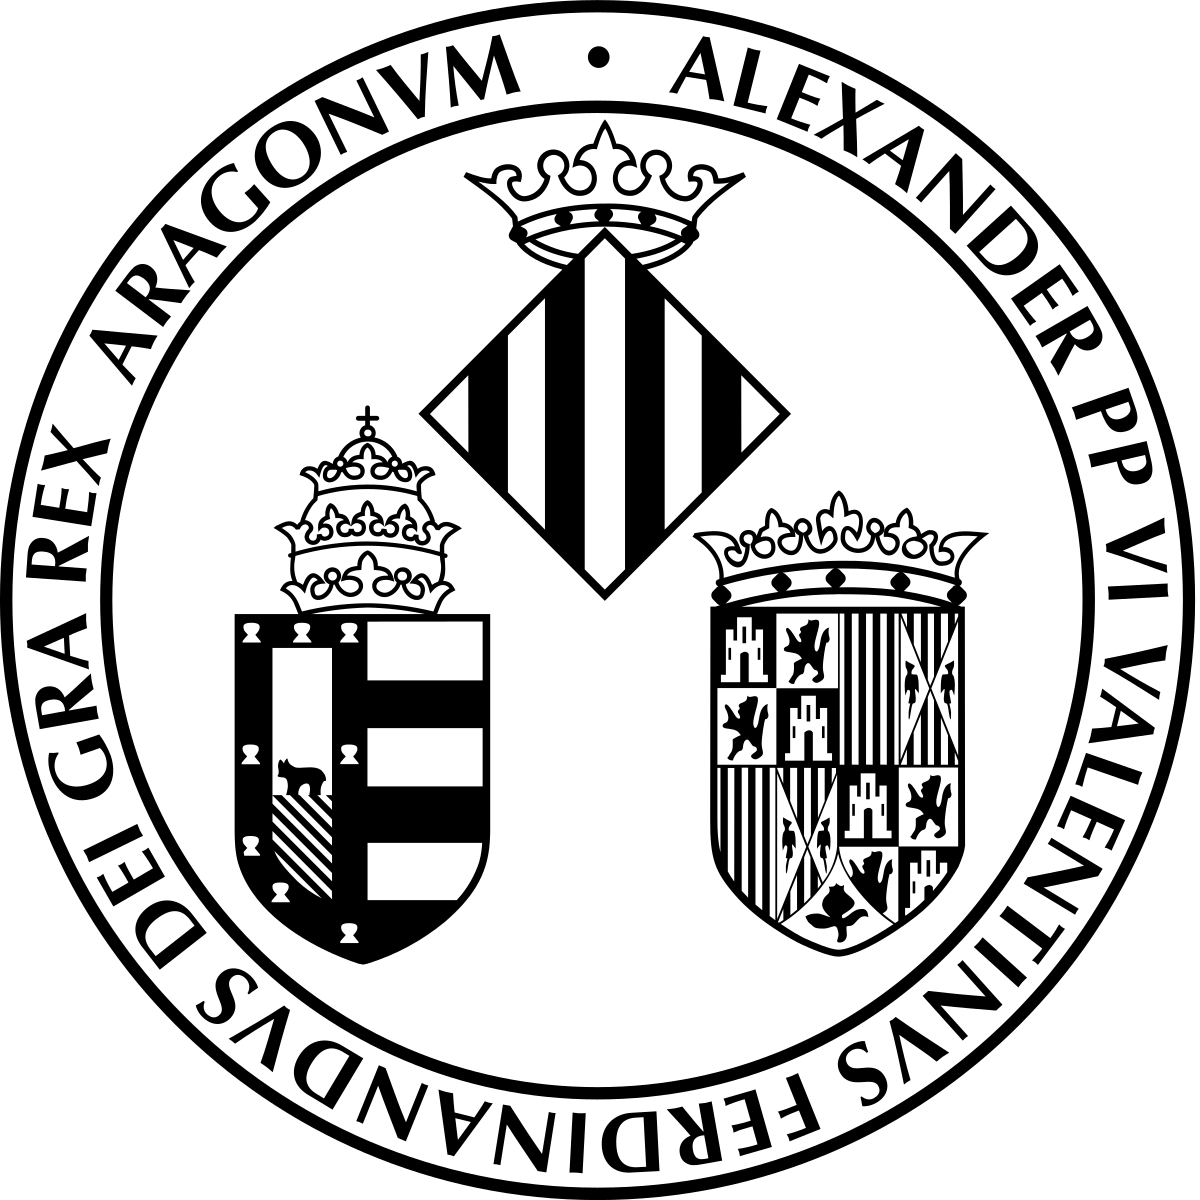
\includegraphics[width=0.5\textwidth]{titlepage/images/logo}
	\end{figure}
	
	\begin{center}
	\textsc{ \LARGE{Universitat de València \\}}
	\textsc{ \LARGE{Escola Tècnica Superior d'Enginyeria \\ }}
	\vspace{5mm}
	{\textsc{PhD Thesis. Doctorat en Enginyeria Electrònica}\\}
	\vspace{40mm}
	\LARGE{\textbf{\@title}}\\ \\
	{\large by Iván Vallés-Pérez \\}
	\vspace{40mm}
	\textnormal{Supervisor: Emilio Soria-Olivas, PhD \\ }
	\textnormal{València - \monthyeardate\today }
	\end{center}

\end{titlepage}
\makeatother
\pagestyle{Preamble}

\tableofcontents
\clearpage

\pagestyle{MyStyle}
%!TEX root = ../thesis.tex
\chapter*{Notation} \label{ch:notation}
We tried to follow a common notation throughout this dissertation. This chapter provides a brief reference of all the conventions followed. 


\section*{Data}

\begin{labeling}{alligator}
	\item [$\mathbf{X}$] a matrix with shape $N \times D$ containing $N$ input row vectors, where each vector is represented as $\{\mathbf{x_1},...,\mathbf{x_i},...,\mathbf{x_N}\}$.
	\item [$\mathbf{x_i}$] a vector of length $D$ where each element represents a particular feature (e.g. age, weight, or IQ of a person).
	\item [$\mathbf{Y}$] a matrix with shape $N \times K$ containing desired output vectors row $\{\mathbf{y_1},...,\mathbf{y_i},...,\mathbf{y_K}\}$.
	\item [$\mathbf{y_i}$]  a vector of length $K$ where each element is one of the scalar desired outputs (e.g. the probability of having a high income in a 5 years time span).
	\item [$\mathbf{T}$] a data set  of examples with inputs and desired outputs for supervised learning tasks, composed of a set of pairs of vectors from $\mathbf{X}$ and $\mathbf{Y}$ matrices grouped as follows: $\{(\mathbf{x_1}, \mathbf{y_1})...,(\mathbf{x_i}, \mathbf{y_i}),...,(\mathbf{x_N}, \mathbf{y_N})\}$, where each tuple represents a training example.
	\item [$\mathbf{U}$] a data set of examples for unsupervised learning tasks, composed of a set of input vectors from $\mathbf{X}$ disposed as follows: $\{\mathbf{x_1},...,\mathbf{x_i},...,\mathbf{x_N}\}$, where each element represents a training example.
\end{labeling}

\section*{Neural networks and machine learning}

\begin{labeling}{alligator}
	\item [$\mathbf{\theta}$] vector containing all the parameters of a neural netword model.
	\item [$f_\mathbf{\theta}(\cdot)$] neural network model with parameters $\mathbf{\theta}$.
	\item [$J(\cdot, \cdot)$] cost function, i.e. differentiable function quantifying the error to be minimized, normally using gradient descent.
	\item [$\mathbf{W}$] weights matrix of a neural network layer, which scalar components are denoted by $w_{ij}$.
	\item[$g(\cdot)$] activation function.
	\item[$G(\cdot)$] multi-layer Perceptron.
	\item[$t$] optimization step.
	\item[$\lambda$] learning rate.
	\item[$m$] minibatch size.
	\item[$L$] number of layers of a deep learning model.
	\item[$\mathbf{h}$] output of a hidden layer.
\end{labeling}


\section*{Calculus}

\section*{Others}
\begin{labeling}{alligator}
	\item [$H$] \textit{Heavyside} function.
	\item [$\sigma(\cdot)$] \textit{Sigmoid} function.
	\item [$\sigma(\tau)$] Hyperbolic tangent function ($\tanh(\cdot)$).
	
\end{labeling}
% !TeX spellcheck = en_US
% !TEX root = ../thesis.tex

\chapter{Introduction} \label{ch:introduction}

\section{Overview}

\subsection{Early artificial intelligence references}
Humans are curious by nature. We have the desire to understand everything around us, from the smallest particle to the vastness of the universe. Our quest for knowledge is what has allowed us to progress as a species and keep evolving. In this journey, we have always looked up at the stars, dreaming of discovering other intelligent beings like us. In this search, we have also looked inward, trying to understand our thoughts, emotions, and the source of our intelligence and consciousness. 

Since ancient times, the human being has dreamed of artificial intelligence (AI). One of the first existing records dates back to \textit{Aristotle} (384–322 BCE) in his book \textit{The Politics}, where the author imagined machines that would think by themselves and act autonomously, with the purpose of allowing humans enjoy leisure \autocite{nils2009}. In 10-70 CE, the mathematician and engineer \textit{Hero of Alexandria} designed several ancient automata \autocite{greenwood1851}, among which stands out an automated theater that would play short performances in front of the audience.

In the 9th century, the three Persian brothers known as \textit{Banū Mūsā} wrote the \textit{book of ingenious devices} \autocite{musa1978}. In their book, they illustrated hundreds of automata along with other mechanical devices (timing and delay devices, automated valves, etc.) and described how those would be used. 

The philosopher, scientist and bishop \textit{Albert Magnus}, in the middle ages (13th century), manufactured several automata. One of the most notorious ones was an artificial talking head able to imitate human voice and breath \autocite{worthies1828}.

Later on, in the renaissance (15th century), the polymath \textit{Leonardo da Vinci} sketched various automata \autocite{nils2009}. His mechanical knight is one of the first anthropomorphic automata we have record of. This automaton was designed to perform basic human-like motions through a system of pulleys and cables. More recently, these sketches have been studied and the mechanical knight has been built faithfully following the original design \autocite{elling2006}, finding that the automaton was fully functional. 

During the 18th century, automata reached a new level of sophistication, the modern history becoming the golden era of automata. One of the most prolific creators was the watchmaker \textit{Pierre Jaquet-Droz} (18th century), who built a number of automata, including a three-year-old child that could write any letter of the alphabet \autocite{carrera1979}.

Years later, other illustrious automata builders of the era were \textit{Wolfgang von Kempelen} (1734-1804), who built \textit{the Turk}, an automaton that could beat any human at chess\footnote{Although after his death, it was discovered that it was actually nothing more than a machine operated by a person from inside a wooden cabinet.} \autocite{jay2000}, 
and \textit{Jacques de Vaucanson} (1709-1782), who built a number of automata, including a duck that could eat and drink \autocite{nils2009, trymbaka2022}. Despite the complexity and ingenuity gained over the years, these automata were all purely mechanical and human operated, without any form of artificial intelligence. 

Fiction stories have often been used as a way to explore the idea of artificial intelligence, and the earliest references in literature date back to the middle ages. In \textit{The City of Brass}, one of the tales included into the \textit{One Thousand and One Nights} (around the 10th century), the main character, a thief, comes across a city ruled by a wizard who created a brass humanoid automaton that could talk and move like a human. In the 19th century, \textit{E.T.A. Hoffmann} (1776-1822) wrote a story entitled \textit{The Sandman} \autocite{hoffmann1816}, where the protagonist falls in love with an automaton created by a professor, without realizing that she was actually a machine. He suffered a mental breakdown after finding out. This automaton, known as \textit{Olympia}, was able to move, talk and sing. In one of the most famous science fiction novels of all times, \textit{Frankenstein}, written by \textit{Mary Shelley} in 1818 \autocite{shelley1994}, the scientist \textit{Victor Frankenstein} creates a human-like creature out of body parts of different people. Although, strictly speaking, \textit{Frankenstein}'s creature is not a machine, it is often seen as one of the first examples of intelligent creations in literature.

A century later, the Czech writer, playwright and critic \textit{Karel Čapek} (1920), wrote a play named \textit{R.U.R.} (\textit{Rossum’s Universal Robots}), which is considered to be the first recorded use of the term \textit{robot}\footnote{The word \textit{robot} is derived from the Czech word \textit{robota}, which means forced labour or slaves.}  \autocite{nils2009}. In that play, robots were manufactured as slaves to do the manual labour that humans disliked. This is often seen as the beginning of the modern science fiction genre.

In 1941, the science fiction writer \textit{Isaac Asimov} published a short story called \textit{Runaround} \autocite{nils2009}, in which he introduced the three laws of robotics (depicted below), which are still considered the basis for the ethical design of robots.

\begin{enumerate}
	\item \textit{A robot may not injure a human being or, through inaction, allow a human being to come to harm}.
	\item \textit{A robot must obey the orders given to it by human beings, except where such orders would conflict with the First Law}.
	\item \textit{A robot must protect its own existence as long as such protection does not conflict with the First or Second Law}.
\end{enumerate}

The above examples are only a few of the many references to artificial intelligence that have been made over the years \autocite{nils2009}. Even though none of these automata were truly intelligent, they represent the beginning of the long and arduous process of building machine intelligence.  

The yearning for artificial intelligence has come and gone in waves over the years, but it has never lost its appeal to human imagination. Each time a new wave of artificial intelligence hits, it brings with it renewed enthusiasm for the possibility that machines can think and act by themselves. 

Recently, artificial intelligence has begun to show significant promise for actually becoming a reality. The history of artificial intelligence is a long one, and its future is still to be written.

\subsection{Modern artificial intelligence}
The dream of AI started to become a reality in the 20th century, with the development of the first computers. In the 1950s, the idea of artificial intelligence was rediscovered by \textit{Alan Mathison Turing} (1912 - 1954), today known as the father of computer science. He secretly defeated the German intelligence's cryptography system (\textit{Enigma} machines; \citealp{Hodges:2000}) and provided a proof showing that it was not possible to find a general solution for the \textit{Hilbert's Entscheidungsproblem} (an important symbolic logic challenge; \citealp{turing1936}). Later, he published the famous article entitled \textit{Computing Machinery and Intelligence} \autocite{turing1950} in which he described a game as a test for machine intelligence. The currently known as \textit{Turing test} consists of an interrogation between a human and an entity (that can either be another human or a machine). The human interrogator's objective is to try to determine, by asking a series of questions, whether the entity it is talking to is a human or a machine. If the interrogator cannot tell the difference (70\% of the times after multiple 5 minutes conversations), then the machine is said to have passed the test, and hence it can be considered intelligent.


The ``artificial intelligence'' term was not coined until 1956 when \textit{John McCarthy} (1927 - 2011) \textit{Nathaniel Rochester} (1919 - 2001) and \textit{Claude Shannon} (1916 – 2001) gave a conference at \textit{Dartmouth College} proposing a 2 month workshop, called the \textit{Dartmouth Summer Research Project on Artificial Intelligence}. This workshop was organized to fund the artificial intelligence as an academic discipline (see the picture in figure \ref{fig:dartmouth_photo}) and the project was fundraised by the \textit{United States Office of Naval Research}. This historical event brought together some of the most prominent computer scientists of the time, including \textit{Marvin Minsky} (1927–2016), \textit{Arthur L. Samuel} (1916–1990), \textit{Ray Solomonoff} (1926-2009) and  \textit{John Nash} (1928-2015), between others\footnote{\textit{John McCarthy}, \textit{Claude Shannon}, \textit{Trenchard More}, \textit{Nathaniel Rochester}, \textit{Oliver Selfridge}, \textit{Julian Bigelow}, \textit{W. Ross Ashby}, \textit{W.S. McCulloch}, \textit{Abraham Robinson}, \textit{Tom Etter},  \textit{David Sayre}, \textit{Kenneth R. Shoulders}, \textit{Alex Bernstein}, \textit{Herbert Simon} and \textit{Allen Newell}.}.

\begin{figure}[h!]
	\centering
	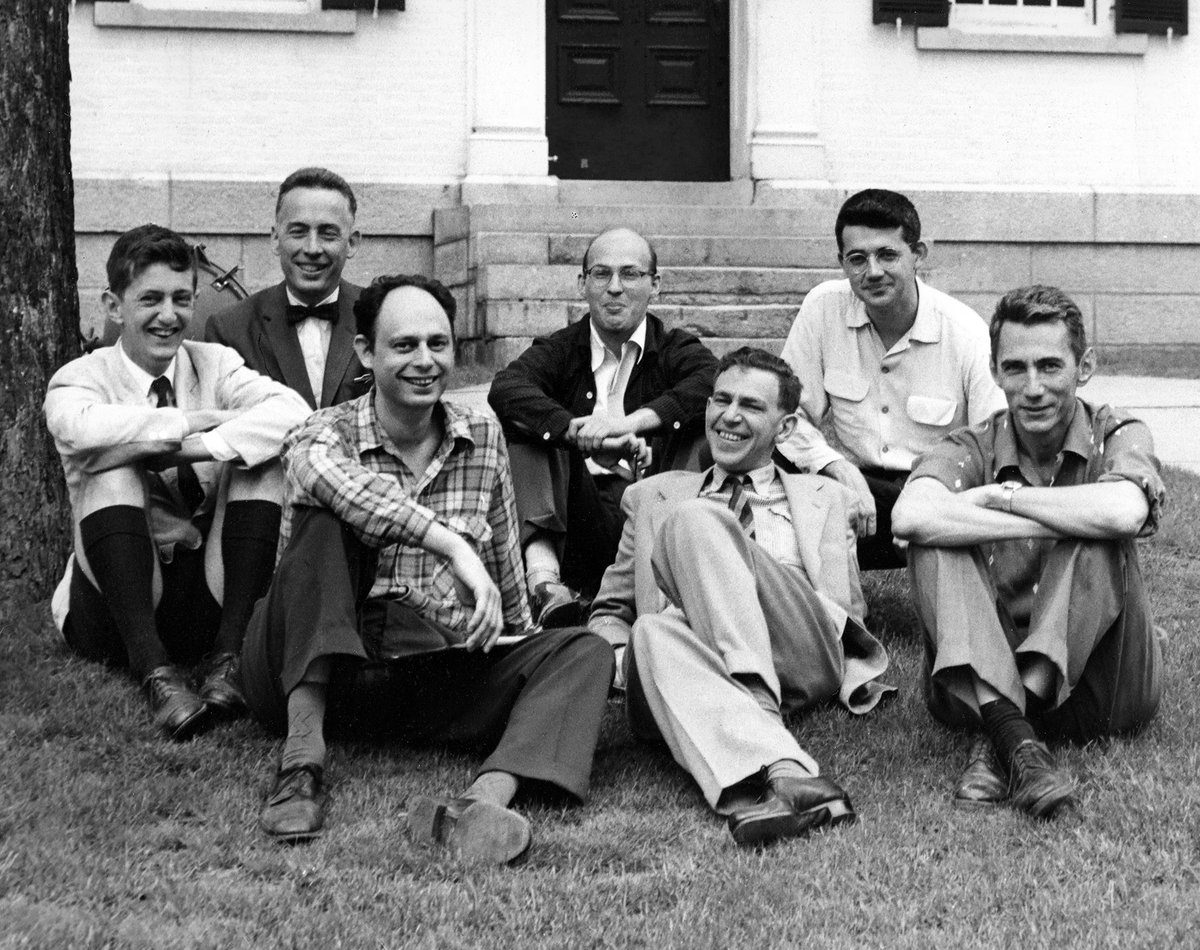
\includegraphics[width=.6\textwidth]{introduction/images/dartmouth}
	\caption[\textit{Dartmouth Summer Research Project on Artificial Intelligence}]{From left to right: \textit{Oliver G. Selfridge}, \textit{Nathaniel Rochester}, \textit{Ray Solomonoff}, \textit{Marvin Minsky}, \textit{Trenchard More}, \textit{John McCarthy} and \textit{Claude Shannon} at the \textit{Dartmouth Summer Research Project on Artificial Intelligence} (Photo: \textit{Margaret Minsky}).}
	\label{fig:dartmouth_photo}
\end{figure}

The recent development of artificial intelligence has not been a linear process and, during its evolution, there have been ups and downs along the way, with several so-called \textit{AI winters}. The \textit{first AI winter} took place between the late 1970s and early 1980s, when research on artificial intelligence came to a standstill. Later, \textit{Sir James Lighthill}, a well-known British scientist, published a report, today known as \textit{the Lighthill report}, concluding that artificial intelligence was a waste of time and money \autocite{lighthillReport}. This publication, together with the oversized expectations for artificial intelligence at the time \autocite{russellNorvig}, led to a decrease of investment for AI research. As a result, the field of artificial intelligence went into decline, stalling for several years.

After the first \textit{AI winter}, the field experienced a revival when several companies started investing in the development of \textit{expert systems}\footnote{A rebranded form of artificial intelligence.}. Software and hardware companies such as \textit{Teknowledge} and \textit{LISP Machines Inc.} grew rapidly during this time in order to meet the rising demand for artificial intelligence technology, which motivated the AI research community to continue with their work. One of the most remarkable inventions of the 80s was the successful application of the \textit{backpropagation} algorithm to neural networks by \textit{David Rumelhart} and \textit{Geoffrey Hinton} \autocite{hinton1986}, which revived the study of artificial neural networks. All this sudden success, together to the collapse of \textit{LISP Machines Inc.} in 1987, led to the \textit{second AI winter}.

The 1990s started with a renewed interest in artificial intelligence and, motivated by the increasing computational power, machine learning algorithms started to be applied to a wider range of tasks \autocite{Tesauro:1995}. Many interesting applications were developed during that decade across several industries like medical diagnosis \autocite{declaris1991, Klein1991, punch1992, Cinar1999}, psychology \autocite{Dorrer1995, denby1999, Ogawa1999, Perlovsky1999}, finance and logistics \autocite{Lipshutz1991, Benaroch1991, Johnson1991, Falas1994} and many others \autocite{Smithers1993, Yoo1994, Mashaly1994, Koyma1998}. Finally, the most sounded event of the 1990s was the victory of the IBM super-computer \textit{Deep Blue} \autocite{Campbell2002} over \textit{Garry Kasparov}, the world chess champion, which took place in \textit{New York City} in 1997. In 1998, \textit{Yann Lecun} and his collaborators published their work on convolutional neural networks \autocite{lecun1999}, a fundamental advance in machine learning which has been widely used in computer vision and other fields. 

The beginning of the 21st century is one of the most fruitful periods for artificial intelligence, with several major achievements in different areas. Further research in neural networks \autocite{hinton2006, hinton2012} gave birth to novel techniques that allowed training deeper models, leading to a rebranding of neural networks as deep learning. In 2011, \textit{IBM's} artificial intelligence program \textit{Watson} won the quiz game \textit{Jeopardy!} against two of the best human players of all time. 

In 2012, \textit{AlexNet} \autocite{krizhevsky2012}, a deep learning model developed by \textit{Geoffrey Hinton} and his collaborators, achieved state-of-the-art performance on the \textit{ImageNet} classification task \autocite{ILSVRC15}, kickstarting the current deep learning revolution. 

In 2016, \textit{Google's} artificial intelligence program \textit{AlphaGo} \autocite{silver2016} defeated the world champion \textit{Lee Sedol} in \textit{the game of Go}, a feat that was considered impossible a few years earlier, by using \textit{reinforcement learning} algorithms. \textit{Alpha Go Zero}, the \textit{Alpha Go's} big brother, proved in 2017 to be more powerful than its predecessor while not needing human interaction to learn \autocite{Silver2017a, Silver2017b}. In 2016, \textit{DeepMind} researchers published \textit{WaveNet} \autocite{vanderoord2016}, a deep auto-regressive model that was able to produce natural raw audio waveforms faithfully generating human speech (a modern version of \textit{WaveNet} has been used in the experiments described in chapter \ref{ch:tts}). One year later, the authors of \citet{vaswani2017} published the transformer, a new architecture designed for sequence transduction tasks that allowed parallel training, as opposed to its sequence-to-sequence predecessors \autocite{sutskever2014}. The transformer architecture has been used in the experiments described in chapter \ref{ch:salesforecast}. In 2020, \textit{OpenAI} researchers published \textit{GPT-3} \autocite{brown2020}, a massive neural network with 175 billion parameters which was able to achieve strong performance on many NLP tasks\footnote{A live example of the power of this model can be found in some of the lines of this chapter, which have been revisited and rephrased with its help.}. Later, in 2021, \textit{AlphaFold} was published by \textit{DeepMind} researchers \autocite{Jumper2021} as a method for inferring the 3D structure of a biological protein based on its genetic sequence, representing one of the major contributions of artificial intelligence to scientific discovery. Finally, in 2022, \textit{OpenAI} researchers published \textit{Dall-e 2}, a text to image generation model able to generate high quality images from textual descriptions \autocite{aditya2022}.

In addition to the mentioned achievements, many algorithms have been published in the generative modeling field. Generative adversarial networks \autocite{Goodfellow2014}, variational auto-encoders \autocite{kingma2019}, normalizing flows \autocite{kingma2016, kobyzev} and diffusion models \autocite{Prafulla2021} are some of the most remarkable examples. Some of these techniques will be discussed in detail in section \ref{sec:generative}.

Many more advances have been made in AI in the past few years, which has led to an increased interest in the technology from both the private and public sectors. However, the application of artificial intelligence to the most complex and important problems still faces many challenges. Here is where deep learning comes into play, as it has shown the ability to achieve state-of-the-art results on a wide range of tasks. Therefore, the development of democratized and low-resource deep learning applications is essential for the future of artificial intelligence. 

Many of the last advances in the deep learning research community report prohibitive amounts of computation needed to train deep learning models \autocite{silver2016, kechyn2018, brown2020, floridi2020}. The authors of \autocite{strubell2019} estimated the amount of $CO_2$ emissions from training a large transformer network (\textit{BERT} size) to be equivalent to the emissions of 5 average cars during all their lifetime, or those of a human during 60 years. 

Research in low-resource deep learning \autocite{howard2017, Han2017, Gao2018, sanchez2020, so2021} has shown the possibility of training deep learning models with a low amount of computation, and its necessity for the future of artificial intelligence, as well as for our planet health.


\section{Contributions}
This dissertation encompasses five contributions to the state of the art of the field of deep learning. Two of them contribute around training methods, and the remaining three are examples of novel applications of deep learning algorithms to industry problems. All the contributions are related to the efficient use of computational resources. Each of these studies is written as a different chapter.

The first contribution (chapter \ref{ch:modulus}) proposes a new activation function for deep learning models: the \textit{modulus} function. The experiments conducted show that, in line with the current research trends, non-monotonic activation functions generally produce better results than monotonic ones. Additionally, the \textit{modulus} activation function is very efficient to compute, as it consists of a single-bit operation, and its derivative (being either 1 or -1) has constant 1-norm. These properties are specially useful for embedded applications. Moreover, the results show that the proposed activation function achieves superior results in computer vision tasks when compared with state-of-the-art alternatives. This work has been published in the journal \textit{Engineering Applications of Artificial Intelligence} \autocite{valles2023a}.

The second contribution (chapter \ref{ch:distillation}) proposes combining the knowledge of several large pre-trained models in order to improve the performance of small low-resource pre-trained models. The results of this chapter show that it is possible to significantly increase the accuracy of the smallest pre-trained models, allowing for computational savings and improved performance.

The first application covered in this dissertation (chapter \ref{ch:salesforecast}) tackles the problem of sales forecasting in the field of logistics. Two end-to-end systems with two different deep learning techniques (sequence-to-sequence models and transformers) are proposed. The results of this chapter conclude that it is possible to build end-to-end systems to predict the sales of multiple individual products, at multiple points of sale and different times with a single machine learning model. The proposed model beats the state-of-the-art alternatives found in the bibliography. This work has been published in the journal \textit{Expert Systems with Applications} \autocite{valles2021c}.

Finally, the last two applications belong to the speech technology field. The former (chapter \ref{ch:kws}) studies how to build a \textit{Keyword Spotting} speech recognition system using an efficient version of a convolutional neural network. In this study, the proposed system is able to beat the performance of all the benchmarks found in the literature when tested against the most complex subtasks. This work has been published in the proceedings of \textit{European Symposium of Artificial Neural Networks (ESANN 2020)} \autocite{valles2021a}. The latter study (chapter \ref{ch:tts}) proposes a standlalone state-of-the-art \textit{text-to-speech} model capable of synthesizing intelligible voice in thousands of voice profiles, while generating speech with meaningful and expressive prosody variations. The proposed approach, removes the dependency of previous models on a second voice generation system, which makes it more efficient at training and inference time, and enables offline and on-device operations. Device-embedded TTS models are important for voice-activated user interfaces, as they provide a more natural user experience due to the reduced latency, while using a fraction of the energy of cloud TTS services. This study was done as part of the work of the author at \textit{Alexa AI} and has been published in the proceedings of \textit{Interspeech 2020} conference \autocite{valles2021b}.

The unpublished works referenced in this section have already been submitted to a journal and, at the time of writing this paragraph, are under revision.

\section{Thesis structure}
This thesis is organized in individual chapters as follows.


\begin{itemize}
	\item \textit{Chapter \ref{ch:background}}: covers the common background needed to understand the methods and algorithms applied in the subsequent chapters.
	\item \textit{Chapter \ref{ch:modulus}}: introduces the \textit{modulus} as activation function, showing its benefits over other alternatives.
	\item \textit{Chapter \ref{ch:distillation}}: studies how to combine pre-trained models using knowledge distillation.
	\item \textit{Chapter \ref{ch:salesforecast}}: explores the application of sequence-to-sequence models and transformers to approach the sales forecasting problem, from an end-to-end perspective. 
	\item \textit{Chapter \ref{ch:kws}}: presents an end-to-end keyword spotting system with convolutional networks.
	\item \textit{Chapter \ref{ch:tts}}: proposes a state-of-the-art multi-speaker text-to-speech (TTS) system with prosody modeling.
	\item \textit{Chapter \ref{ch:conclusions}}: wraps the general conclusions of the studies presented in the previous chapters.
\end{itemize}


     


% Todo: add references to my papers
% Todo: update current state of the papers
% !TeX spellcheck = en_US
% !TEX root = ../thesis.tex
\chapter{Background} \label{ch:background}
\section{Machine learning}
Human beings learn by experience, part of which is inherited from previous generations. However, in the digital world, experiences can be stored in form of data, which can be later processed and analyzed.

We live in the middle of a data deluge. The technological progress and the internet have boosted our logging and communication capacities. At the time of writing this paragraph\footnote{https://www.internetlivestats.com/one-second/ on February 6th 2022}, every single second 10,000 new tweets are written, 100,000 search queries are sent to \textit{Google}, 100,000 videos are being viewed in \textit{YouTube}, and 3,000,000 emails are sent. All amounts to approximately a 140 terabytes of internet traffic per second.

This \textit{Brobdingnagian} amount of data cannot be analyzed without the help of automated computational assisted tools, and this is exactly the purpose of machine learning. More formally, we define machine learning as a set of computational methods designed to automatically learn hidden structures and patterns from the data and its origin \autocite{murphy2012, theodoridis2015}. Machine learning algorithms can serve multiple purposes ranging from informing decision making under uncertainty to understand and simulate natural processes. Sometimes, machine learning algorithms are inspired in biological processes or in how the brain works and learns \autocite{haykin1998} (e.g. \textit{self-organizing maps} \autocite{kohonen2001}). Other times, machine learning is driven by specific needs arising from data analysis problems (e.g. binary decision trees \autocite{hastie2009, hastie2014}).

\section{Types of learning}
Machine learning algorithms are designed to learn from data. However, there are many ways these data can be treated in the learning process. In this section, the most common types of learning are described at a high level.

\subsection{Supervised learning}
Supervised learning is the most widely employed methodology to train machine learning models. It is based on a function-fitting perspective, where the function $f_\theta$ is adjusted (or trained, in machine learning jargon) to map a set of input vectors $\mathbf{X}$ to the corresponding output vectors $\mathbf{Y}$ ($f_\theta:\mathbf{X}\rightarrow \mathbf{Y}$), given a set of $N$ input pairs $\mathbf{T}=\{(\mathbf{x_i},\mathbf{y_i})\}_{i=0}^{N}$ known as the training dataset \autocite{theodoridis2015}. The learning algorithm adjusts the parameters $\mathbf{\theta}$ of a function $f_\theta$ according to the minimization of a predefined cost function $J$ (for example the mean squared error between the predicted values and the labels) \autocite{hastie2009}. The vector $\mathbf{x_i}$ (with length $D$, $\mathbf{x_i} \in \mathbb{R}^D$) represents a set of features (e.g. the age and the income of a person)  and $\mathbf{y_i}$ (with length $K$, $\mathbf{y_i}\in\mathbb{R}^K$) is the vector of response variables (representing for instance the probabilities to buy a set of products)\footnote{Notice that we represent the output $\mathbf{y_i}$ as a vector although supervised models can be univariate. However the multivariate form is a more general case.}.

There are two main forms of supervised learning  \autocite{murphy2012}.

\begin{itemize}
	\item \textit{Regression}, where the task consists of mapping each input vector $\mathbf{x_i}$ to a real-valued vector $\mathbf{y_i} \in \mathbb{R}^K$. An example of this task would be predicting the age of an \textit{abalone}\footnote{a type of marine snail} based on physical measurements of the different parts of its body \autocite{dua2019abalone}.
	\item \textit{Classification}, where a task consists of mapping the input vectors $\mathbf{x_i}$ to nominal variables from a finite set $\mathbf{C_j}$, $y_{i,j} \in \{1,2,...,||\mathbf{C_j}||\}$, where $||\mathbf{C_j}||$ is the cardinality of the $j$-th response set. An example of a classification task would be determining if a mushroom is poisonous or edible based of several physical characteristics \autocite{dua2019abalone}.
\end{itemize}

\subsection{Unsupervised learning}
Unsupervised learning techniques are employed when no labeled data is available. The training dataset is composed of a set of input vectors $\mathbf{U}=\{(\mathbf{x_i})\}_{i=0}^{N}$, and the objective consists of finding interesting patterns in the data. Compared to supervised learning, unsupervised learning comprises a wider range of techniques and its objective is less well defined: the models have no clear desired output nor obvious error metric \autocite{Goodfellow2016}. However, the unsupervised learning paradigm seems to be closer to the way animals and humans learn. These algorithms also provide a cheaper framework for data exploitation, given that no data annotation is required by human experts, which is generally expensive.

Some of the most common applications of unsupervised learning are described below.

\begin{itemize}
	\item \textit{Clustering}: consists of finding dissimilar subpopulations in the data (also known as clusters or groups), where the elements within a subpopulation are more similar between them than to elements in other subpopulations.
	\item \textit{Density or probability mass estimation}: the machine learning algorithm is trained to learn the probability density function of the data (or the probability mass function in case $\mathbf{X}$ is discrete) $p_{model}(\textbf{X}): \mathbb{R}^N \rightarrow \mathbb{R}$ \autocite{Goodfellow2016}. For this, the model needs to learn the underlying structure of the data $\mathbf{X}$. The techniques laying in this family can be used for many downstream applications, such as clustering \autocite{wang2006}, missing data imputation \autocite{qichuan2015} or generation \autocite{liu2020a}.
	\item \textit{Manifold learning}: is a set of techniques consisting of learning the structure of high-dimensional data, where the data is assumed to lie on a low-dimensional manifold in a high-dimensional space \autocite{murphy2012}. The objective of these techniques is to discover latent structures in the data that can be exploited for tasks such as data compression, dimensionality reduction, feature extraction or data visualization. One example of this task could be reducing the dimensionality of a dataset using \textit{principal components analysis} (PCA). That would project the original dataset into a linear lower dimensional one with orthogonal axes, where the structures in the data could presumably be more easily discernible.
	\item \textit{Data completion}: consists of imputing the missing values of a given dataset \autocite{vanburen_2018}. This can be done with different purposes such as inferring the unfilled optional answers of a survey, or filling the gaps of a time series with low sampling frequency to get a higher time resolution representation. Some forms of collaborative filtering \autocite{falk2019}, for example matrix factorization algorithms \autocite{koren2009}, can also be seen as a data completion task where the algorithm needs to fill the blanks of a matrix representing the ratings of products by customers. In these cases, the algorithm needs to answer a question similar to: what would be the rating that a given customer would assign to a given product if they had the chance?
	\item \textit{Associative learning}:  is a type of unsupervised learning where the goal is to discover the relationships between objects in the data \autocite{zhang2002}. These relationships can be expressed in terms of associations (e.g. if A then B), correlations (e.g. A is positively correlated with B) or co-occurrence (e.g. A and B are often observed together). One example of associative learning would be applying the \textit{Apriori} algorithm \autocite{agrawal1996} to a supermarket database in order to discover the most interesting associations between different products with the aim of deriving attractive offers for customers, or optimize product placement to improve customer experience. 
	\item \textit{Generative modeling}: many forms of generative model also rely on unsupervised learning techniques \autocite{bishop2006}. This task consists of learning to approximate $p(\mathbf{X})$ with the objective of generating data that is indistinguishable from the original distribution. It is often done by maximizing the likelihood of the data given the model $\mathrm{argmax}_\mathbf{\theta} p(\mathbf{\mathbf{X},\mathbf{\theta}})$, however, in cases where the explicit density function is not needed, other methods may apply (this topic will be covered more in depth in section \ref{sec:generative}).  One example of application of these techniques would be in the field of natural language processing, where the goal is to learn a model that can generate text \autocite{uday2019} that is realistic and linguistically plausible (these are commonly known as language models).
\end{itemize}


\subsection{Reinforcement learning}
Reinforcement learning is a family of machine learning algorithms which, in contrast to the other types of learning, does not necessarily rely on any previously gathered knowledge about the task at hand. Instead, the reinforcement learning agents (or decision makers) learn what to do by mapping situations to actions \autocite{sutton2018} so that they maximize a numerical reward metric, usually in presence of uncertainty \autocite{haykin1998}. For the agent to learn successful behaviors (referred commonly as policies), it needs to balance exploration and exploitation while interacting with the environment \autocite{sutton2018}, in simpler terms, reinforcement learning algorithms learn by trial and error.

More formally, the environment is commonly formulated as \textit{finite-discrete-time Markov decision process} \autocite{haykin1998}, which can be represented as a 4-tuple: ($S$, $A$, $P_a$, $R_a$) where $S$ represents the state space, $A$ is the action space, $P_a(s, s')$ is the probability of transitioning from state $s$ to state $s'$ after performing the action $a$, and $R(s, s', a)$ is the reward received when transitioning from state $s$ to state $s'$ after performing action $a$. 

The objective of the learning algorithm is to build an agent such that its policy $\pi_\theta(s)$ maximizes the expected sum of discounted rewards $\mathbb{E} \left[ \sum_{t=0}^{T} \gamma^t R(s_t, s_{t+1}, a) \right]$, where $\gamma$ is usually a scalar number between 0 and 1. The reinforcement learning theory is originally based upon dynamic programming \autocite{szepesvari2010}.

A classical example of a successful reinforcement learning application can be found in \autocite{tesauro1994}, where an agent is trained to play \textit{Backgammon} game.

Detail treatment of the reinforcement learning field lies far beyond the scope of this thesis, a more detailed introduction is given in \autocite{sutton2018, szepesvari2010}.

\subsection{Other types of learning} \label{sec:typesoflearning_others}
There are other learning paradigms \autocite{raghu2020} that are worth mentioning, but either it is not clear where they lay, or they combine elements from various of the previously discussed types of learning. The following list describes the most important ones.
\begin{itemize}
	\item \textit{Semi-supervised learning algorithms} learn from both labeled and unlabeled data. This is beneficial in problems where it is difficult or costly to label the data, and hence the amount of labeled data is scarce \autocite{raghu2020}. One example of field where semi-supervised learning has many potential applications is fraud detection \autocite{wang2020b}, where these cases are uncommon by nature, and difficult to spot.
	\item \textit{Self-supervised learning algorithms} aim to solve what is known as a \textit{pretext task}: a supervised problem where the data can be automatically labeled without human intervention, without extra cost and directly from the raw instances \autocite{raghu2020}. One example of \textit{pretext task} could be determining the missing word in a partially masked sentence, given a set of sentences extracted from a collection of books \autocite{devlin2019}, with the aim of learning latent representations of the words. Other example could be determining the degree of rotation of an image \autocite{gidaris2018} for biasing the model towards learning the latent structure of the images.
	\item \textit{Transfer learning} is a discipline solely applicable to deep learning models. This methodology consists of two steps: pre-training a model to solve a large and generic task (e.g. classify large and full-color images into 1000 categories \autocite{deng2009imagenet}) and then fine-tuning the pre-trained model to solve a different target task \autocite{raghu2020}. This paradigm has a lot of benefits in multiple applications (for instance when restricted amounts of labeled data are available, or when the computational resources available are limited). As an example, the authors of \autocite{souza2022} show how they got successful results in performing sentiment analysis over user reviews by using pre-trained word embeddings based on \textit{BERT} \autocite{devlin2019}. Further details about transfer learning will be covered in the chapter \ref{ch:distillation} of this thesis.
\end{itemize}


\section{Deep learning}

Deep learning algorithms were motivated by the failure of classical machine learning algorithms on solving central problems on AI (e.g. speech recognition, object recognition, text generation, etc). These algorithms have a long history (figure \ref{fig:dl-timeline} summarizes the most important events in the development process of deep learning), and have been named differently along the years: connectionist models, artificial neural networks, deep learning, etc.

\begin{figure}
	\centering
	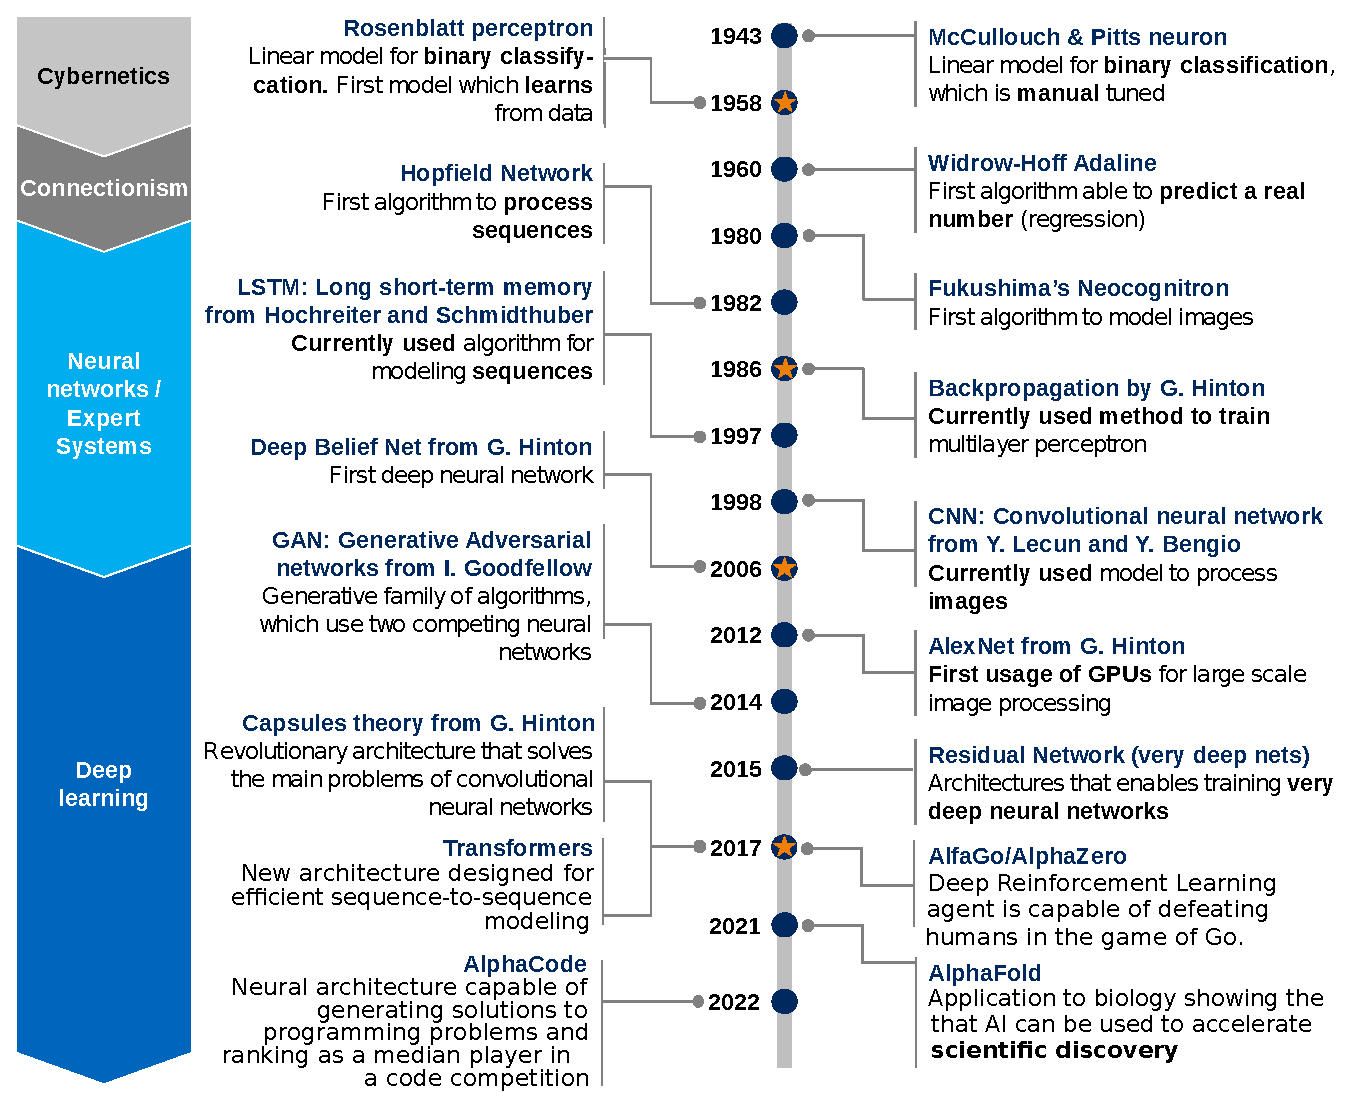
\includegraphics[width=1.0\linewidth]{background/images/DL-timeline}
	\caption[Deep learning history timeline]{Timeline showing the most important achievements in the research of what is currently known as deep learning.}
	\label{fig:dl-timeline}
\end{figure}


Deep learning is a subfield of artificial intelligence and machine learning as shown in the \textit{Venn} diagram of figure \ref{fig:venndl} (taken from \cite{Goodfellow2016}), and provides a very flexible framework for different machine learning tasks, spanning all the aforementioned types: supervised, unsupervised, reinforcement learning and others.

\begin{figure}
	\centering
	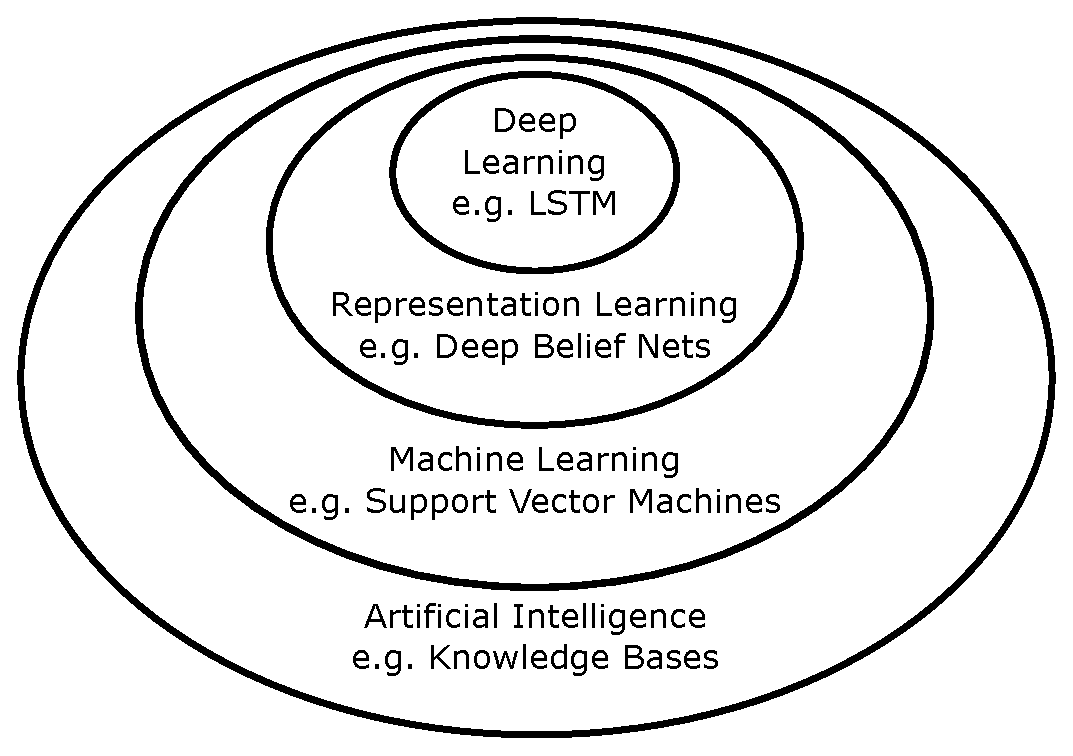
\includegraphics[width=0.5\linewidth]{background/images/venn_DL}
	\caption[Deep learning \textit{Venn} diagram]{Deep learning context within the artificial intelligence field \autocite{Goodfellow2016}}
	\label{fig:venndl}
\end{figure}



\subsection{From the perceptron to its multilayer version} \label{sec:mlp}

This section introduces the basic feed-forward neural network, from its origin to the modern trends. The basic component of a modern deep learning model is the artificial neuron (sometimes called unit). The idea of an artificial neuron has its origin in the \textit{McCulloch-Pitts} model from 1943, an attempt to mathematically model the functionality of a biological neuron \autocite{mccullochPitts1943}. The \textit{McCulloch-Pitts} neuron consisted of a linear function of a set of binary inputs $\mathbf{x}$ that are multiplied by a set of weights $\mathbf{W}$ (which values are either excitatory or inhibitory, i.e. 1 or -1), the result is added together, a threshold scalar is subtracted to the result, and a sign function is applied to produce a binary output $y$ (see figure \ref{fig:mcpittsneuron} for a graphical description). The whole model is described in equation \ref{eq:mcpitts}. This weights and the threshold were meant to be adjusted manually by an operator.

\begin{figure}
	\centering
	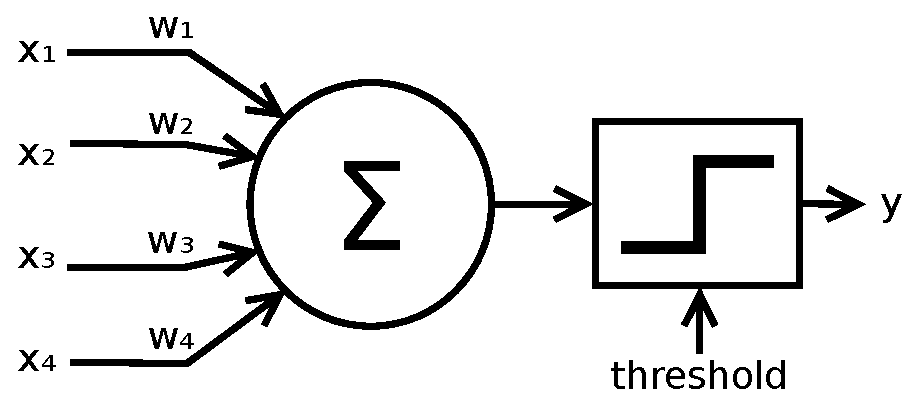
\includegraphics[width=0.60\linewidth]{background/images/mcpittsneuron}
	\caption[\textit{McCulloch-Pitts} neuron model]{\textit{McCulloch-Pitts} neuron model, with 4 input variables $\{x_i\}$ and one output $y$. $\{w_i\}$ represent the synaptic weights of the neuron.}
	\label{fig:mcpittsneuron}
\end{figure}

\begin{equation}
	\label{eq:mcpitts}
	y_i = \mathrm{sgn}\left(\sum_{j=1}^{D} x_{i,j} \cdot w_{j} - \mathrm{threshold}\right)
\end{equation}

Some years later (1958), \textit{Frank Rosenblatt} introduced the \textit{perceptron} \autocite{Rosenblatt58}. His idea builds upon the \textit{McCulloch-Pitts} model, proposing a simple method to automatically learn the weights of the model (see equation \ref{eq:rosenblatt}, where the desired response is represented by $y_j$, the predicted one is represented by $\hat{y}_j$ and $\lambda$ is a scalar that controls the size of the weight updates, commonly referred as the learning rate). This is considered the first primitive neural network.

\begin{equation}
\label{eq:rosenblatt}
\mathbf{w_j(t+1)} = \mathbf{w_j(t)} + \lambda [ y_j-\hat{y}_j(t) ] \cdot \mathbf{x_j}
\end{equation}

 A couple of years later, \textit{Bernard Widrow} and his student \textit{Ted Hoff} proposed the \textit{ADALINE} model (ADAptive LINear Element) \autocite{widrow1960}, a modification of the \textit{McCulloch-Pitts} model that removed the sign function. \textit{ADALINE} was trained using gradient descent \autocite{fredric2000}, as described in equations \ref{eq:adaline_gd} and \ref{eq:adaline_step}, where $\lambda$ is the learning rate and $N$ is the number of training examples (these equations are commonly known as \textit{the delta rule}).
\begin{equation}
\label{eq:adaline_fp}
y_i = \sum_{j=1}^{D} x_{i,j} \cdot w_{j} + b
\end{equation}

\begin{equation}
\label{eq:adaline_gd}
\frac{\partial J}{\partial{w_j}} = \frac{1}{N} \sum_{i=1}^{N} x_{i,j} \cdot(\hat{y}_i - y_i)
\end{equation}

\begin{equation}
\label{eq:adaline_step}
\mathbf{w_j(t+1)} = \mathbf{w_j(t)} - \lambda \cdot \frac{\partial J}{\partial {w_j}}
\end{equation}


 The combination of multiple \textit{ADALINE}-style perceptrons with activation functions such as the sigmoid function (see equation \ref{eq:mlp}, where $g$ represents a non-linear activation function), builds a \textit{multilayer perceptron} (\textit{MLP}). More specifically, a \textit{MLP}, also known as \textit{fully-connected} neural network, is a neural architecture which building blocks are perceptrons (called neurons in this scenario) which are disposed in layers so that all the elements from a layer $l$ are connected with all the elements in the next layer $l+1$ (refer to figure \ref{fig:mlp} for a visual example)


 \begin{equation}
 \label{eq:mlp}
 h_i = g\left(\sum_{j=0}^{D} x_{i,j} \cdot w_{j} + b\right)
 \end{equation}

 The \textit{delta rule}, described in equations \ref{eq:adaline_fp} and \ref{eq:adaline_gd}, built the basis for the \textit{backpropagation} algorithm, a widely used methodology nowadays as standard method to train neural networks. The \textit{backpropagation} algorithm \autocite{hinton1986} was published by \textit{David Rumelhart} and \textit{Geoffrey Hinton} in 1986 as a method to optimize the parameters of \textit{multilayer perceptrons}. This algorithm consists of two steps \autocite{haykin1998}:

\begin{enumerate}
\item \textit{Forward pass}: consisting of a simple model inference operation, where a set of features $\mathbf{x}_i$ are feed to the network as input to get the output $\mathbf{\hat{y}_i}$. In this phase, some of the values of the intermediate neurons can be cached to use them in the next step.

\item \textit{Backward pass}: a metric $J$ (often referred as cost or loss function) is used to compare the outputs of the model $\mathbf{\hat{y}_i}$ with the desired outputs (sometimes called targets) $\mathbf{y_i}$ and then propagate the gradient of the error backwards (from the output to the input), by using the chain rule, to adjust the weights of the model.
\end{enumerate}


\begin{figure}
	\centering
	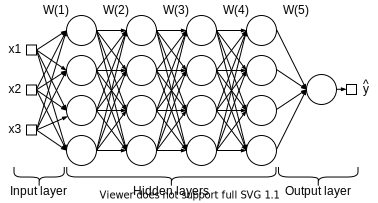
\includegraphics[width=0.8\linewidth]{background/images/mlp}
	\caption[Multilayer perceptron]{Example of \textit{multilayer perceptron} with 3 inputs, 1 output and 3 hidden layers. Each bubble represents a neuron (figure \ref{fig:mcpittsneuron}), and has an associated bias term. Each arc represents a weight. In each neuron, the inputs multiplied by their corresponding weights are added to the neuron's bias, and then an activation function is applied to produce the output, according to equation \ref{eq:mlp}.}
	\label{fig:mlp}
\end{figure}


Before \textit{backpropagation}, there was no algorithm for training \textit{multilayer perceptrons} in an end-to-end manner. The only way to train those models was to fix the weights of all but one layer, and train the free one with gradient descent or other methods. These models were called feature analyzers \autocite{hinton1986}, and one of the most interesting examples is the \textit{Gamba} perceptrons, described in \autocite{minsky69}. Although it is out of the scope of this thesis, it may be worth mentioning that modern versions of the \textit{Gamba perceptron} (known as \textit{Extreme Learning Machines}) are still in the research community spectrum as alternative training methods to \textit{backpropagation} see \autocite{Huang2006, Huang2012}.

The introduction of \textit{backpropagation} enabled the neural networks to learn their own hidden representations automatically, allowing for more complex and abstract models. One of the most important pieces of \textit{multilayer perceptrons} and other modern architectures are the neuron \textit{activation functions} (also referred sometimes as \textit{nonlinearities}). An \textit{ADALINE} style neuron is a linear function, and linear functions are closed under composition, therefore the composition of several \textit{ADALINE} neurons is a linear function. To break the linearity of the neurons, the \textit{activation functions} are introduced. They consist of non-linear functions which are applied to the output of each neuron. The authors of \autocite{hinton1986} formulated the \textit{backpropagation} algorithm with sigmoid activation functions (defined in equation \ref{eq:sigmoid}), as a differentiable alternative to the classical sign function. Later, it was discovered that unbounded and non-smooth \textit{nonlinearities} like the \textit{Rectified Linear Unit} (\textit{ReLU}) \autocite{nair2010} (defined in equation \ref{eq:relu}) were more convenient for training deep architectures \autocite{Goodfellow2016}. Activation functions are discussed in depth in chapter \ref{ch:modulus}.


\begin{equation}
\label{eq:sigmoid}
f(x) = \frac{1}{1+e^{-x}}
\end{equation}

\begin{equation}
\label{eq:relu}
f(x) = \max(x, 0) =
\begin{cases}
x,          & \text{if } x \geq 0 ,\\
0,         & \text{otherwise},
\end{cases}
\end{equation}

The \textit{backpropagation} algorithm has certain rules that need to be met \autocite{hinton1986}: (1) connections from higher level neurons to lower level ones are forbidden, but connections that skip layers are totally permitted, (2) the architecture must be fully differentiable to be able to backpropagate the errors and (3) the weights must not be initialized to constant values, but they must be set to random values instead, to break the symmetrical weights between layers (which would cause the optimization to stall, see \autocite{hinton1986} for more details). 

Despite meeting these rules, there are no theoretical guarantees for the algorithm to find the global minimum, it can get stuck in local minima. One possible way to avoid this problem consists of running the optimization several times with different random parameter initializations \autocite{haykin1998}. The usage of gradient-free methods such as evolutionary optimization techniques \autocite{sivanandam2008} have also been explored by the deep learning research community, sometimes leading to promising results \autocite{omid2014, vallesperez2012}. However, these algorithms are usually less computationally efficient than gradient-based ones, making them unfeasible when the training data or the model size are large.

\subsection{Neural networks as universal approximators}
Given any continuous function $f(x)$ with arbitrary complexity, it is always possible to find a multilayer perceptron with a single hidden layer and sigmoid activations that approximates that function to any desired degree of accuracy.

This problem was originally formulated and solved by \textit{G. Cybenko} \autocite{Cybenko1989}. In particular, he proved that:

\begin{thm}[ 2 - Cybenko, 1989]
	Let $\sigma$ be any continuous sigmoidal function. Then finite sums of the form

	$$ G(x) = \sum_{j=1}^{N} \alpha_j \sigma(w_j^Tx + \theta_j) $$

	are dense in $C(I_n)$. In other words, given any $f \in C(I_n)$ and $\epsilon > 0$, there is a sum, $G(x)$, of the above form for which

	$$|G(x) - f(x)| < \epsilon \quad \forall x \in I_n$$
\end{thm}

For the sake of gaining intuition (refer to \autocite{Cybenko1989} for a formal proof), let $G$ be a \textit{multilayer perceptron} with a single hidden layer, which neurons have a sigmoid activation. Assuming the weights of the hidden layer are set to a sufficiently large number, it can be easily seen that the sigmoid activations approximate a \textit{Heavyside step function} $H$ (see equation \ref{eq:sigmoidToHeavyside}, where $\delta$ represents a very large number). Then, by adding many \textit{Heavyside} functions with the proper shift and scaling, one can easily approximate any continuous function. It can be also seen that the shift and scaling operations correspond to the bias of the neurons in the hidden layer and the weights of the output layer, respectively. See figure \ref{fig:universalapprox} for a graphical example. 

As it can be seen, by increasing the number of neurons one can easily control the fidelity of the approximation. This theorem proves that if we have enough neurons in the hidden layer, a \textit{multilayer perceptron} with only one hidden layer can approximate any continuous function to an arbitrary degree of precision.


\begin{figure}[h!]
	\centering
	\includegraphics[width=1\linewidth]{background/images/universalapprox}
	\caption[Universal approximation theorem visual example]{In the left side, a toy \textit{multilayer perceptron} with a single hidden layer, a single input and a single output, and with the weights of the hidden layer set to a very large number $\delta$. The bias terms have been indicated inside the bubbles. In the right hand side, a target function $f(x)$ to be approximated (smooth dashed blue line) and the approximation $G(x)$ (thick solid line) achieved given the weights and biases in the network of the left. The different segments of the approximation have been colored with the same color as the last neuron that fired to set that value, as the value of $x$ increases.}
	\label{fig:universalapprox}
\end{figure}

\begin{equation}
	\label{eq:sigmoidToHeavyside}
	\lim_{\delta \rightarrow \infty} (\sigma(\delta x)) = \mathrm{H}(x)
\end{equation}



After \textit{Cybenko}, other studies \autocite{Leshno1993, pinkus1999} proved that the theorem holds for non-sigmoid activation functions as well. Despite the universal approximation theorem proving that a single hidden layer is enough to model any arbitrarily complex continuous function, deeper neural networks are motivated by the fact that more sophisticated functions may approximate complex problems more easily and efficiently, perhaps even needing less parameters \autocite{nguyen21}.



\subsection{Deeper neural networks} \label{sec:deepernn}
Regardless the emergence of the \textit{backpropagation} algorithm, training a \textit{multilayer perceptron} with many layers was \textit{challenging}. The first successful methodology for training deep neural networks consisted on pre-training the weights of the network in an unsupervised fashion, using stacks of \textit{restricted Boltzmann machines} (RBM) \autocite{Smolensky1986} known as deep belief networks \autocite{hinton2006, Bengio2007}. A \textit{restricted Boltzmann machine} (initially called \textit{Harmonium}) is a type of neural network built using a bidirectional bipartite graph architecture, with symmetric connections of neurons between the two layers and without connections between neurons within the same layer (as shown in figure \ref{fig:rbm}). This model is trained to learn hidden abstract representations of the input, from which it is possible to recover the original probability distribution $p_\theta(x|h) \approx p(x)$. The training procedure is based on an approximate \textit{maximum-likelihood} method called \textit{contrastive divergence} (CD) \autocite{hinton2002}.

\begin{figure}[h!]
	\centering
	\includegraphics[width=0.3\linewidth]{background/images/rbm}
	\caption[\textit{Restricted Boltzmann machine}]{\textit{Restricted Boltzmann machine} with 5 visible units and 3 hidden units.}
	\label{fig:rbm}
\end{figure}

Deep belief networks are stacks of RBMs that are trained using a greedy layer-wise strategy, in which the output of a trained RBM becomes the input of the following RBM \autocite{hinton2006} (see figure \ref{fig:dbn}). It was shown in \autocite{Bengio2007} that by following this procedure and then fine-tuning the weights of the full network using the backpropagation algorithm, deeper networks could be trained.


At the time of writing this thesis, unsupervised pre-training methods are no longer needed to train deep neural networks. This is thanks to a set of techniques that have been recently developed (in the 21st century) and that when combined together, facilitate the convergence of the \textit{backpropagation} algorithm when used to optimize deep architectures. The first technique was the \textit{ReLU} \autocite{nair2010} activation functions (see equation \ref{eq:relu}), a non-saturating alternative to the classical functions like \textit{sigmoid} (see equation \ref{eq:sigmoid}) or \textit{tanh}, that showed to be effective at favoring sparse connectivity, and helped overcome the saturating gradients problem, a well known failure mode of neural architectures with saturating \textit{nonlinearities} when trained by \textit{backpropagation} \autocite{Hong2019}. Another simple technique that helped training deep neural networks is known as \textit{Dropout}, a regularization technique that consists of randomly zeroing out a fraction $p$ of neurons from each layer in each training step \autocite{hinton2012, srivastava2014}. These two techniques (among others) allowed \textit{Alex Krizhervsky} and collaborators to successfully train \textit{AlexNet} \autocite{krizhevsky2012} without unsupervised layer-wise pre-training, a deep neural network that won the \textit{ImageNet} \autocite{deng2009imagenet} computer vision contest in 2012, a problem consisting of classifying millions of images into 1,000 categories. These techniques are still used today in the majority of the deep learning models that are published.

\begin{figure}
	\centering
	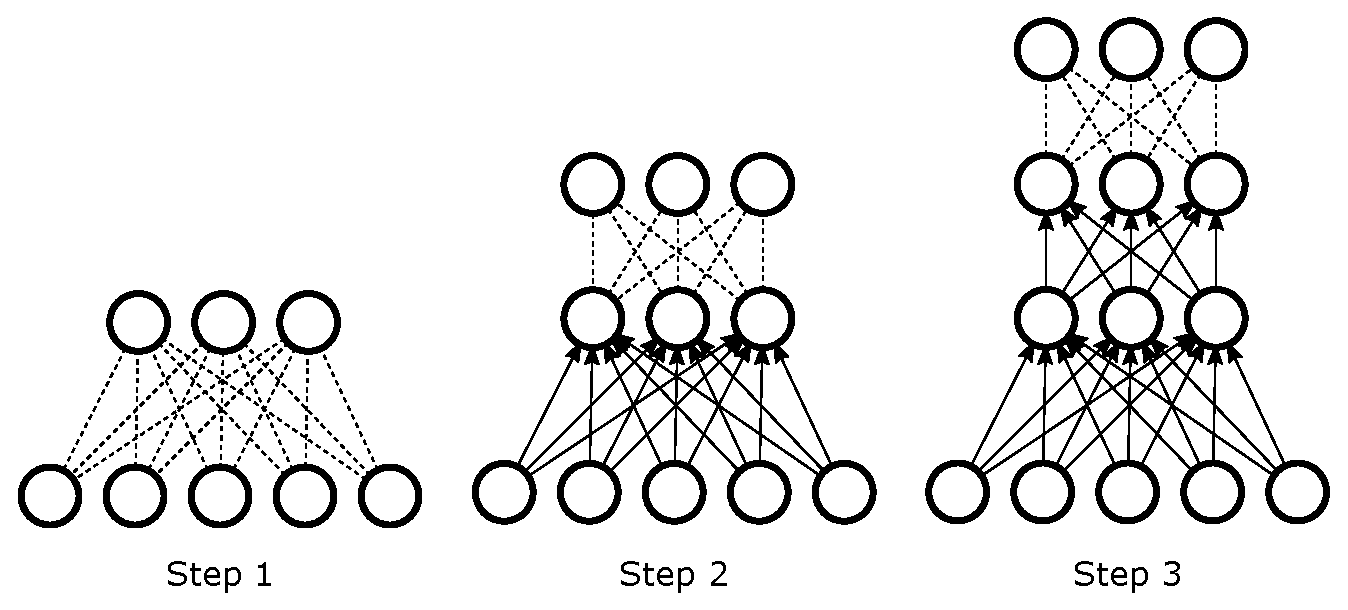
\includegraphics[width=1\linewidth]{background/images/dbn}
	\caption[Deep belief network]{Example of \textit{deep belief network} architecture with three feature detector layers. In each of the steps shown above, the dashed connections between units represent the \textit{RBM} being trained, while the solid connections represent the previously trained \textit{RBMs} that are used to compute the input of the next \textit{RBM}.}
	\label{fig:dbn}
\end{figure}



Other tricks that are commonly used nowadays to facilitate the parameters optimization of deep architectures are batch normalization \autocite{ioffe2015} and residual learning \autocite{kaiming2016}. 
\begin{itemize}
	\item \textit{Batch normalization} consists of standardizing the output vectors from hidden layers using the first and the second statistical moments (mean and variance) of the current mini-batch \autocite{ioffe2015}. This method has proved to increase the training stability when high learning rates ($\lambda$) are used \autocite{Goodfellow2016}. Additionally, it has been shown that it provides regularization \autocite{dauphin2021} as a side effect, due to the random fluctuations in the statistical moments from one batch to another.
	\item \textit{Residual learning} consists of adding skip connections between layers of the neural network, so that the output of one layer $l$ is fed as input to layer $m > (l+1)$. Figure \ref{fig:residual} shows an example of a graph with a residual block skipping two layers. More formally, the output of the residual block becomes $\mathbf{H(x)} = \mathbf{F(x)} + \mathbf{x}$ where $\mathbf{F(x)}$ is the function learned by the composition of the two layers and the \textit{ReLU} function\footnote{notation disambiguation: $H(x)$ here does not refer to the \textit{Heavyside} function}. Obviously one can see that $\mathbf{F(x)}$ is learning a residual mapping $\mathbf{F(x)} = \mathbf{H(x)} - \mathbf{x}$ \autocite{kaiming2016}. This method has empirically shown substantial improvements of the \textit{backpropagation} optimization process given that the residual connections allow gradients to flow more easily, avoiding vanishing gradients \autocite{Goodfellow2016}. The authors of \autocite{kaiming2016} were able to get the first place in the 2015 \textit{ImageNet} contest, improving the performance of \textit{AlexNet}. Recent studies found that residual connections help reform the loss landscape leading to more convex optimization surfaces \autocite{freeman2017, wang2020a}.
\end{itemize}
 


\begin{figure}[h!]
	\centering
	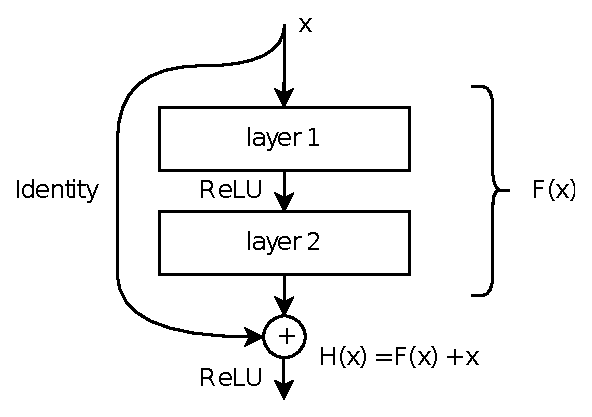
\includegraphics[width=0.5\linewidth]{background/images/residual}
	\caption[Example of a residual block]{Example of a residual block.}
	\label{fig:residual}
\end{figure}


Finally, another difference between modern and classical deep learning models is the extended use of \textit{mini-batch} stochastic gradient descent (see equation \ref{eq:mbsgd}), where successive optimizations steps are performed by \textit{backpropagation} using small ($m$-sized) random subsamples of the dataset named \textit{mini-batches} \autocite{ruder2016}. Previous alternatives were stochastic gradient descent, where the updates are performed for every individual sample, and batch gradient descent, where the updates are performed over the full dataset $\mathbf{T}$. \textit{Mini-batch} gradient descent has shown generalization improvements over the batch method \autocite{Hoffer2017}, while being computationally more efficient than the \textit{stochastic gradient descent} method.


\begin{equation}
	\label{eq:bgd}
	\mathbf{\theta}(t+1) = \mathbf{\theta}(t) - \lambda \cdot \nabla_\mathbf{\theta} J(X, Y|\mathbf{\theta}(t))
\end{equation}

\begin{equation}
	\label{eq:sgd}
	\mathbf{\theta(t+1)} = \mathbf{\theta}(t) - \lambda \cdot \nabla_\mathbf{\theta} J(x_i, y_i|\mathbf{\theta}(t)) \quad \mathrm \quad \mathrm{where} \quad (\mathbf{x_i}, \mathbf{y_i}) \sim \mathbf{T}
\end{equation}

\begin{equation}
	\label{eq:mbsgd}
	\mathbf{\theta}(t+1) = \mathbf{\theta}(t) - \lambda \cdot \nabla_\mathbf{\theta} J(x_{i:i+m}, y_{i:i+m}|\mathbf{\theta}(t)) \  \mathrm{where} \quad  (\mathbf{x_{i:i+m}}, \mathbf{y_{i:i+m}}) \sim \mathbf{T}
\end{equation}


\subsection{Modern architectures}
In this subsection three modern building blocks frequently used in the current deep learning architectures are described from a general perspective: convolutional neural networks (CNN), recurrent neural networks (RNN) and transformers. These architectures are the backbone of the majority of deep learning applications and the computational core of the systems presented throughout the next chapters.

\subsubsection{Convolutional neural networks}
A CNN is a type of feed-forward neural network that is commonly used in problems where the input data have grid-like topology \autocite{Goodfellow2016}. Common examples of these data are time-series (1D), images (2D) or videos (3D). CNNs are not new, and one of the most important primitive CNN is known as \textit{neocognitron}, a neural architecture published by \textit{Kuniko Fukushima}, as a model inspired in the primary cortex of the human brain that was able to recognize Japanese handwritten characters \autocite{fukushima1980}. This model was similar to modern convolutional neural networks, and even featured similar properties like weight sharing and translation equivariance (these properties are discussed below). The \textit{neocognitron} inspired future works like \textit{LeNet-5}, a 7-layer convolutional neural network (see figure \ref{fig:lenet5}) trained with \textit{backpropagation} to recognize handwritten digits \autocite{lecun1998}.

\begin{figure}
	\centering
	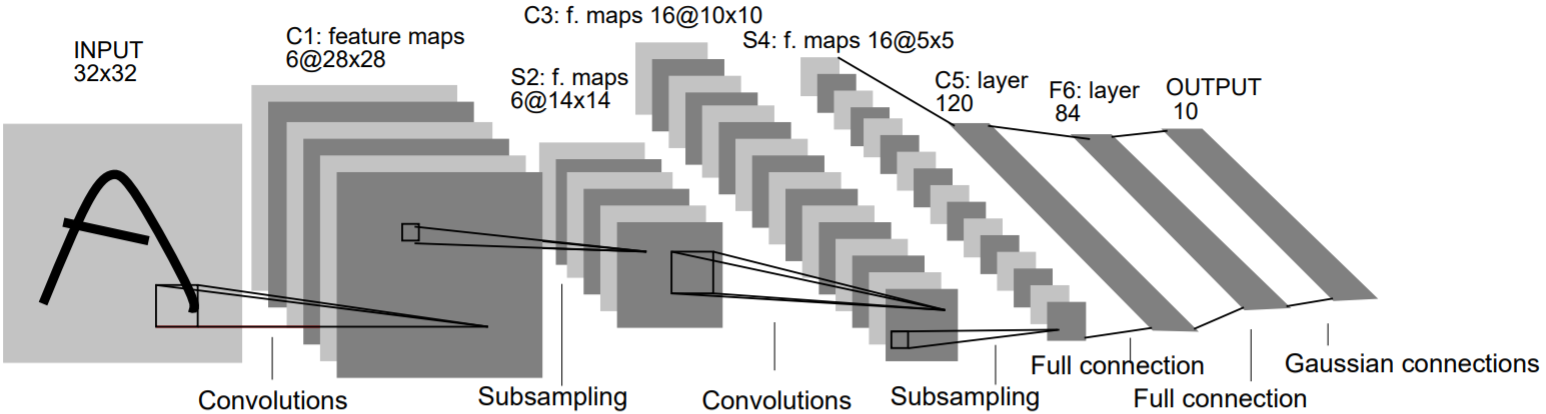
\includegraphics[width=0.85\linewidth]{background/images/lenet5}
	\caption[\textit{LeNet-5} architecture]{\textit{LeNet-5} neural architecture, with 7 layers, capable of recognizing handwritten digits.}
	\label{fig:lenet5}
\end{figure}

CNNs use cross-correlation operations\footnote{Formally, the operation is called cross-correlation, however they are more commonly referred as convolutions by the machine learning community.} instead of the general matrix multiplication used in fully connected networks. In this context, a convolution is a linear operation where an input $\mathbf{X}$ is correlated with a \textit{kernel} $\mathbf{W}$ to produce a \textit{feature map} $\mathbf{S}$ (see equation \ref{eq:cnnformula}, where $g$ represents the \textit{nonlinearity}). The task of the algorithm is to learn the \textit{kernel} to solve the target task \autocite{haykin1998}. In other words, equation \ref{eq:cnnformula} describes how the \textit{kernel} is displaced over the input image $\mathbf{X}$ to determine its similarity with the different regions of the full-color image.

\begin{equation}
	\label{eq:cnnformula}
	S_{i,j.k} = g\left(\sum_{l,m,n}{X_{i+l, j+m, k+n} \cdot W_{l,m,n} + b}\right)
\end{equation}

The convolutional neural networks are composed (sometimes partially) of convolutional layers (where several convolutional \textit{kernels} are applied in parallel). These layers have several properties that differenciate them from the classical dense layers, and that become advantageous when the input data can be arranged into a grid structure. These properties are discussed below \autocite{Goodfellow2016}.


\begin{itemize}
	\item \textit{Sparse interactions}: the units in a convolutional network are connected to a small region of neighboring inputs. The size of that region is commonly referred as \textit{receptive field}. This property drastically reduces the amount of parameters of the neural network, and enables parameters sharing.
	\item \textit{Parameter sharing}: consists of using the same parameters for more than one function in the model. This is also known as \textit{tied weights}. In a CNN, each member of the kernel is used at each position in the input (except in the special case of the boundaries, depending on the setting).
	\item \textit{Equivariance to translation}: the convolution operation builds a map representing the positions where a certain feature appears in the input (e.g. a vertical border in the case of an image). If the feature is moved in the input, its representation will be moved the same amount in the output representation. Notice that the convolution operation is not equivariant to other transformations such as rotation and scaling. This lack of properties inspired the development of the \textit{capsule networks} \autocite{sabour2017}.
\end{itemize}

Apart from the convolutions, there is another operation that is commonly used in CNNs known as subsampling. Its goal is to reduce the size of the feature maps as more layers are added, so that the representations become more generic. This helps achieve approximate invariance to translation. There are two main versions of this operation: pooling or strided convolutions. The pooling operation \autocite{Goodfellow2016} consists of computing a reducing statistic (e.g. the $\max$ function in max-pooling) over small neighboring regions. The strided convolutions \autocite{riadh2020} are standard convolutions that skip some of the inputs.

In some CNN architectures, a couple of fully-connected layers are added on top of the convolutional layers. Although, recent advances in the field have found that this is not necessary \autocite{shelhamer2015}, this pattern is commonly seen in modern architectures.

% TODO: Add modern CNN graph (maybe)

\subsubsection{Recurrent neural networks}
\sloppy RNNs are one type of neural networks that are designed to process sequential data such as time-series: $x^{(1)}, x^{(2)}, ..., x^{(T)}$, where $T$ represents the time series length. One of the most important primitive version of RNNs is known as the \textit{Hopfield} network \autocite{hopfield1982} and was published in 1982. This network incorporated a memory cell that allowed it to process sequential data. However, it was initially designed to work with binary data.

Inspired by the \textit{Hopfield} network and its variants, the current RNNs are also incorporate memory cells (sometimes referred as the RNN internal state) that allow them to process variable-length sequences such as text sentences or audio clips \autocite{haykin1998}.

A RNN shares its weights across several time steps. This may sound similar to 1-dimensional CNNs (1D-CNNs), but there is one important difference \autocite{Goodfellow2016}. In a 1D-CNN layer, each of the elements of the output sequence is function of a small number of neighboring elements in the input sequence, whereas in the basic RNNs each element in the output is function of all the previous elements in the sequence; in other words, RNNs are causal. 

A recurrent neural network takes one input each time step, and then passed to a hidden layer that produces an output, see equation \ref{eq:RNN} for a basic example of recurrent neural network ($\mathbf{U}$ and $\mathbf{W}$ represent the trainable weight matrices, $\mathbf{b}$ is a trainable bias vector, and $\mathbf{h}$ represents the hidden intermediate representation). These hidden representations are designed to retain the important information of the previous sequence steps in order to solve the required task.

\begin{equation}
\label{eq:RNN}
\mathbf{h^{( t )}} = \mathbf{g(U h^{( t-1 )}} + \mathbf{W x^{( t )}} + \mathbf{b})
\end{equation}

The most commonly used type of recurrent neural network nowadays is the \textit{long short term memory} (LSTM). LSTMs were published by  \textit{Hochreiter} and \textit{Schmidhuber} \autocite{Schmidhuber1997} in an attempt to solve the issues of RNNs when dealing with sequences in problems that required long-term dependencies. LSTM models contain two hidden state representations: one intended to retain long term memory and other for short term memory. The architecture of a LSTM cell is composed of three gates: input gate $\mathbf{i_t}$, output gate $\mathbf{o_t}$, forget gate $\mathbf{f_t}$. These gates control how the information flows through the network, allowing to write, output and delete the states as needed. This is made possible due to the sigmoid functions, which act as valves for the different operations. Figure \ref{fig:lstm} and equations \ref{eq:LSTM} describe the LSTM cell more formally. In the equations, the symbol ``$\odot$'' refers to the \textit{Hadamard} product, $\mathbf{U}$ and $\mathbf{W}$ are trainable weight matrices, and $\mathbf{b}$ are the biases.

\begin{figure}
	\centering
	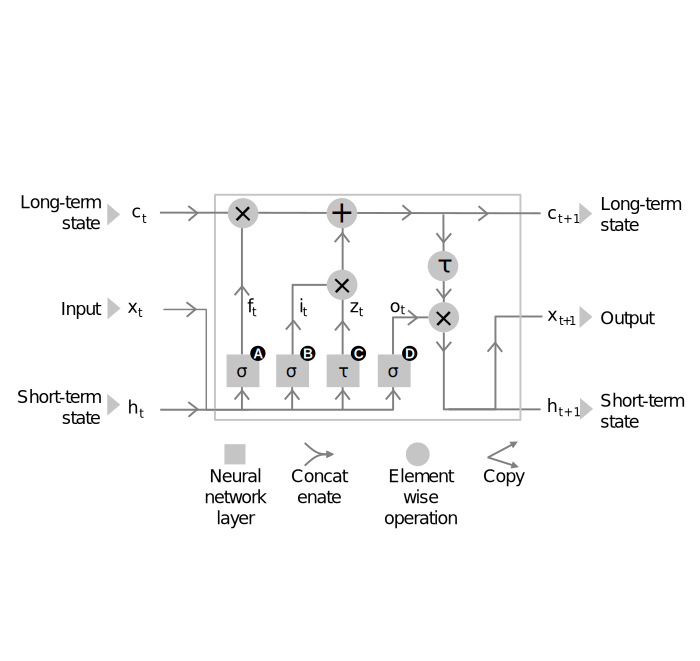
\includegraphics[width=0.7\linewidth]{background/images/LSTM}
	\caption[LSTM cell structure]{LSTM cell structure. $\mathbf{c_t}$ and $\mathbf{h_t}$ represent the long-term and short-term states, respectively, that the network uses as memory. Its operation is based on 3 gates and an output unit. (A) is a layer that acts as forget gate, represented as $\mathbf{f_t}$, which is responsible for erasing memory which will no longer be used. The layer (B) is the input gate, represented as $\mathbf{i_t}$, and controls how much input goes through the long-term line. The layer (C), represented by $\mathbf{z_t}$, controls the new contribution to the cell state that, in conjunction with the layer B form the memory addition system. The layer (D), represented as $\mathbf{o_t}$ is the output gate, which controls which values are outputted. In the diagram, $\sigma$ stands for the logistic function and $\tau$ for the hyperbolic tangent.}
	\label{fig:lstm}
\end{figure}



\begin{align}
\label{eq:LSTM}
\begin{split}
	\mathbf{f_t} &= \sigma(\mathbf{W_f} \mathbf{x_t} + \mathbf{U_f} \mathbf{h_{t-1}} + \mathbf{b_f})\\
	\mathbf{i_t} &= \sigma(\mathbf{W_i} \mathbf{x_t} + \mathbf{U_i} \mathbf{h_{t-1}} + \mathbf{b_i})\\
	\mathbf{o_t} &= \sigma(\mathbf{W_o} \mathbf{x_t} + \mathbf{U_o} \mathbf{h_{t-1}} + \mathbf{b_o})\\
	\mathbf{c_t} &= \mathbf{f_t} \odot \mathbf{c_{t-1}} + \mathbf{i_t} \circ \tau (\mathbf{W_c} \mathbf{x_t} + \mathbf{U_c} \mathbf{h_{t-1}} + \mathbf{b_c})\\
	\mathbf{h_t} &= \mathbf{o_t} \odot \sigma(\mathbf{c_t})
\end{split}
\end{align}

Apart from the LSTM, there are other more modern variants that are gaining popularity. One of them is the \textit{gated recurrent unit} (GRU) \autocite{chung2014} a recurrent cell similar to the LSTM but more efficient and with a single state signal that showed to be as effective as its predecessor. Depending on the application, the recurrent layers can be bidirectional, allowing the network to process the sequences in a forward and backward fashion \autocite{schuster1997}.

\subsubsection{Transformer} \label{sec:transformer}
A transformer \autocite{vaswani2017} is a neural architecture with encoder-decoder structure that allows mapping sequence-to-sequence \autocite{sutskever2014} problems without the need of sequential models such as RNNs. These models make use of attention and self-attention mechanisms \autocite{bahdanau2015} to process and align the input and output sequences, and allow processing the sequential data in parallel at training time, at the cost of a higher memory consumption\footnote{the self-attention operation computational and memory complexity depend quadratically on the length of the sequences}. The basic transformer  architecture is shown in \ref{fig:transformer}. The original proposal is defined for natural language processing tasks, however it has been shown that it can be used for other purposes with simple modifications \autocite{naihan2019, jiarui2021, sanyuan2021}.

\begin{figure}
	\centering
	\includegraphics[width=0.8\linewidth]{background/images/transformer}
	\caption[Transformer architecture]{Transformer architecture as defined in \autocite{vaswani2017}. The left module represents the encoder and the right module represents the decoder. In the figure, $Nx$ represents the number of times the encoder and decoder blocks are repeated in cascade. Typically $Nx=8$. }
	\label{fig:transformer}
\end{figure}

As opposed to RNNs, that use their state vectors to process the sequence steps in a sequential manner, transformers use \textit{multi-head attention} (MHA) directly on the projected inputs (input embeddings). This removes the sequential dependencies of the algorithm (needing to run part of the computation graph to be able to compute the following piece) allowing parallel computation \autocite{uday2019}. In this setting, the input and output sequences are computed using self-attention and then, the encoder and decoder vector spaces are combined with another attention mechanism.

 \textit{Multi-head attention} is defined as an operation over three matrices: the query $\mathbf{Q}$, the key $\mathbf{K}$ and the value $\mathbf{V}$. The name of these matrices comes from an analogy to information retrieval systems, where input queries (usually in form of a text sequence) are used to find the best matching key and value (representing a document name and content, respectively) \autocite{manning2008}. In the attention mechanism a similar process happens, where the query is compared against all the keys to produce an \textit{attention vector} $\mathbf{a} \in \mathbb{R}^{d_{\mathrm{model}}}$ such that $\sum_{i} a_i = 1\ \mathrm{and}\ 0<a_i<1\ \forall\ i$, which is used to weight the values corresponding to the keys \autocite{vaswani2017}. See equation \ref{eq:mhaconcat} for a more formal definition. Notice that the original definition of the transformer \autocite{vaswani2017} uses \textit{scaled dot product}  to calculate the similarity between the queries and the keys. This operation is defined in \ref{eq:scdotprod} and does not require any parameter: it is a dot-product operation normalized by the length of the sequences $d_k$ (see figure \ref{fig:attentionmodules} for a visual description). Refer to table \ref{table:attentionsimilarities} for alternative similarity metrics that are commonly used in the attention mechanism \autocite{uday2019}.

 \begin{equation}
 \label{eq:mhaconcat}
 \mathrm{MHA}(\mathbf{Q, K, V}) = \mathrm{Concatenate}(\mathrm{\mathbf{head_1}},\mathrm{\mathbf{head_2}},...,\mathrm{\mathbf{head_s}})
 \end{equation}


 \begin{equation}
 \label{eq:headsdef}
 \mathrm{\mathbf{head_i}}(\mathbf{Q,K,V}) = \mathrm{Attention}(\mathbf{Q} \mathbf{W^Q_i}, \mathbf{K} \mathbf{W^K_i}, \mathbf{V} \mathbf{W^V_i})
 \end{equation}

 \begin{equation}
 \label{eq:scdotprod}
 \mathrm{Attention}(\mathbf{Q, K, V}) = \mathrm{softmax} \left(\frac{\mathbf{QK}^T}{\sqrt{d_k}}\right) \cdot \mathbf{V}
 \end{equation}



Figure \ref{fig:transformer} shows how the different modules are arranged in the transformer architecture. In particular, $Nx$ MHA blocks with residual connections form the encoder and the decoder modules, and each MHA block is followed by a fully connected layer that combines the output of all the heads of the MHA. A very important detail is that the decoder self-attention needs to be \textit{masked} so that the whole operation is causal (i.e. each output element strictly depends on the previous input elements, and not on the present or future ones) \autocite{vaswani2017}. The mask, together with the shift of the input sequence (so that the output of the transformer at time step $t$ is calculated taking the $0..t-1$ input elements into account), allow the parallel training of the transformer.

Given that the scaled dot product operation is not location-aware, positional encodings are added to the embedding inputs, to allow the model to sort correctly the input signals if needed.

\begin{table}
\caption[Attention similarity metrics]{Attention similarity metrics \autocite{uday2019}.}
\footnotesize
\centering
\begin{tabular}{r|lll}
	\toprule
	                        Name & Definition                                                                                        & Parameters                           & Ref                     \\ \midrule
	           Concat & $score(\mathbf{q}, \mathbf{k}) = \mathbf{v^T} \tanh(\mathbf{W}([\mathbf{q};\mathbf{k}])$          & $\mathbf{v}, \mathbf{W}$             & \autocite{Luong2015}    \\
	           Linear  & $score(\mathbf{q}, \mathbf{k}) = \mathbf{v^T} \tanh(\mathbf{W}\mathbf{q} + \mathbf{U}\mathbf{k})$ & $\mathbf{v}, \mathbf{W}, \mathbf{U}$ & \autocite{bahdanau2015} \\
	   Bilinear & $score(\mathbf{q}, \mathbf{k}) =  \mathbf{q^T} \mathbf{W} \mathbf{k}$                             & $\mathbf{W}$                         & \autocite{Luong2015}    \\
	       Dot & $score(\mathbf{q}, \mathbf{k}) = \mathbf{q^T}  \mathbf{k}$                                        & None                                 & \autocite{vaswani2017}  \\
	Scaled dot   & $score(\mathbf{q}, \mathbf{k}) =  \mathbf{q^T} \mathbf{k} / \sqrt{d_k}$                           & None                                 & \autocite{Luong2015}    \\ \bottomrule
\end{tabular}
\label{table:attentionsimilarities}
\end{table}

As it can be noticed in equation \ref{eq:scdotprod}, the dot-product used to compute the attention similarity scores makes quadratic the memory requirements and computational cost  (for the case of the self-attention) on the length of the input and output sequences. This is not a desirable property, and the authors warn about it in the paper \autocite{vaswani2017}, becoming one of the major limitations of this approach. There are already studies in the literature that discuss how to reduce that cost \autocite{jaegle2021, so2021}.

\begin{figure}
	\centering
	\includegraphics[width=0.85\linewidth]{background/images/attention_modules}
	\caption[Transformer building blocks]{Left: the scale dot product computation graph (same as equation \ref{eq:scdotprod}). Right, the multi-head attention module (see equation \ref{eq:mhaconcat}).}
	\label{fig:attentionmodules}
\end{figure}

% TODO: Add bias variance tradeoff section and a model capacity one.
\subsection{Deep generative models} \label{sec:generative}
Generative modeling with deep learning is one of the most current trending topics in the machine learning research community. The models in this family learn the probability distribution over multiple variables of the data, in one way or another. From an intuitive perspective, to generate new data a generative model needs to grasp a deep understanding of the structure of that data distribution \autocite{Goodfellow2016}.

The goal of the deep generative models is to learn to approximate the probability of the data ($p_\mathrm{data}$) in an unsupervised way. In other words, the data generator needs to find $\theta$ so that $p_\mathrm{data}(x) \approx p_\mathrm{model}^\theta(x)$ given a metric of similarity \autocite{Goodfellow2016}. The general framework consists of collecting a large amount of data samples from a specific domain and train a deep learning model that is able to generate new data that \textit{looks like}\footnote{we will revisit the problem at the end of this chapter.} the original data.

The family of deep generative models is very diverse, and the models can be categorized into different types depending on the way they solve the generative task. Figure \ref{fig:generativetaxonomy} shows the taxonomy of the type of models discussed in this subsection. Some of the models allow evaluating the learned probability of data $p^\theta_\mathrm{model}(x)$ explicitly, others give an approximation for that distribution, and the others do not provide a way to interact with the probability density, yet allowing operations such as sampling from the implicit probability distribution \autocite{Goodfellow2016}. This subsection provides a description of the following families of deep generative models: \textit{fully visible belief networks} (FVBN), \textit{variational auto-encoders} (VAE), \textit{generative adversarial networks} (GAN) and \textit{normalizing flows} (NF).

\begin{figure}[h!]
	\centering
	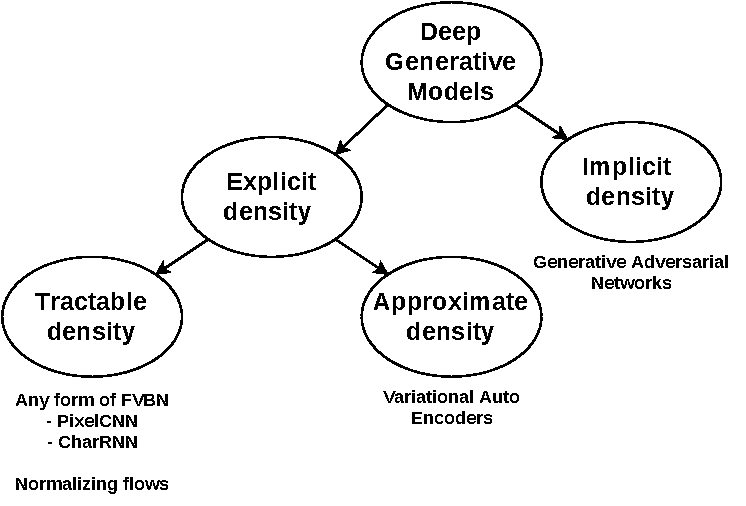
\includegraphics[width=0.85\linewidth]{background/images/generativetaxonomy}
	\caption[Taxonomy of deep generative models]{Taxonomy of the most common deep generative models.}
	\label{fig:generativetaxonomy}
\end{figure}


\subsubsection{Fully Visible Belief Networks}
The \textit{fully visible belief networks} (FVBN) are a family of probabilistic models that use the chain rule of probabilities to model the probability density of the data ($p_\mathrm{model}(x) \approx p_\mathrm{data}(x)$) \autocite{smith2018}. For that, $p_\mathrm{model}(x)$ is decomposed into a set of conditional probabilities $p(x^{(t)}| x^{(1)}, x^{(2)}, \ldots, x^{(t-1)})$ that when multiplied together form  $p_\mathrm{model}(x)$, as shown in equation \ref{eq:fvbn}.

\begin{equation}
	\label{eq:fvbn}
	p_{model}(x) = \prod_{i=1}^{T} p(x^{(t)}| x^{(1)}, x^{(2)}, ..., x^{(t-1)})
\end{equation}

The FVBN models provide a fully tractable probability density function \autocite{Goodfellow2016}, and are well suited for modeling sequential data such as text or speech \autocite{Wang2017,Shen2018,liu2019b}. They have also been applied to model images, by turning them into sequences of pixels \autocite{Oord2016, Oord2016b}.

The basic operation of FVBN is very simple. At training time, a model is trained to predict the next sample of a sequence $x(t)$, given the previous samples $ x^{(1)}, x^{(2)}, ..., x^{(t-1)}$. This operation is known as \textit{teacher forcing} \autocite{williams1989, Goyal2016, Goodfellow2016}, as the model is feed with the original samples of the sequence being modeled. At inference time, a start sample $\hat{x}^{(1)}$ is provided as input for the model to predict a probability distribution $p(x^{(2)}|\hat{x}^{(1)})$ from which the next sample is drawn $\hat{x}^{(2)}$. Subsequently, $ \hat{x}^{(1)}$ and $\hat{x}^{(2)}$ are feed into the model to get the probability distribution of the third sample $p(x^{(3)}|\hat{x}^{(1)}, \hat{x}^{(2)})$, from where $x^{(3)}$ is drawn. The process continues until a stop criterion is reached. The inference operating mechanism is commonly referred \textit{free running mode} \autocite{Goodfellow2016}, as the model is feed with previously generated samples, and does not depend on the ground truth signal. Normally, a deep learning model is used to train FVBN, in particular RNNs and transformers are some of the most common choices. Figure \ref{fig:charrnn} shows an example of \textit{char-rnn} \autocite{Sutskever2011, Graves2013}, a FVBN used to generate natural language. 

\begin{figure}
	\centering
	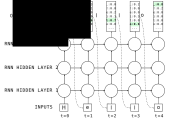
\includegraphics[width=0.8\linewidth]{background/images/char_rnn}
	\caption[\textit{Char-rnn} architecture]{Architecture of \textit{char-rnn}, a deep learning model used for natural language generation at character level, based on a multilayer recurrent neural network. The nodes represent RNN cells (e.g. GRU cells) and the rectangles are the inputs and outputs of the model. The dashed arrows represent the character sampling process.}
	\label{fig:charrnn}
\end{figure}


As it can be noticed, the training process, provided with the right algorithms, can be performed in parallel. However, the inference process needs to be done sequentially, given that to generate future samples, all the past samples need to have been previously generated. For this reason, FVBN are known to be inefficient at inference time when used to generate long sequences.

As an example, a shallow version of the \textit{char-rnn} model of order\footnote{the probability distribution of the next character is conditioned to the previous 100 characters} 100 has been trained using 800 books from the open source \textit{Gutenberg} project\footnote{https://www.gutenberg.org/} \autocite{gerlach2020}. The model consists of a recurrent neural network that is trained to predict the \textit{Multinoulli} distribution for the next character, conditioned to the previous 100 characters as input. The code of this model can be found in the repository linked in the footnote\footnote{\url{https://github.com/ivallesp/simple_chatbot}}. The following is an example of generation where the first 100 characters of the \textit{War of the Worlds} book from \textit{Herbert George Wells} are feed as input.

\chapquote{\textbf{``No one would have believed in the last years of the nineteenth century that this world was being wat}ched together far out
	to the thought, 'that will cled it announced for them bloody I have
	last instant all the strayes as thomass us? This is, and the single
	War camp, until we proguted it toward the mouncin to lint of the
	enemy respectful, then the ribonament had been their courts and papers
	she been ended bent tense freely after good to the eyes to avole.
	The gather flooded by Wayer a great time home engaged in the
	exhausting day of the dutie of summers and jangers untourant altogether
	of mountains. But was the mystery arising half die for some regarding
	the raider. This top was a Catelumberhand life by the river were
	business, and other ebbsake and septimum at the campaich, wa, and he
	showed my brethren.''}{\textit{char-rnn}}{2017}

It can be noticed that the model has been able to generate many grammatically correct words, however the text generated is not coherent. For that, more sophisticated approaches would be needed. \textit{GPT-3} \autocite{floridi2020} is a modern example of deep language model.

Other example of modern FVBN application is \autocite{Oord2016, Oord2016b}, an extension of \textit{char-rnn} to two dimensions, where a set of pixels of an image are given as input to the model, and its task is to predict the remaining pixels in an auto-regressive manner. 


\subsubsection{Variational auto-encoders}
\textit{Variational auto-encoders} (VAE hereafter) are another alternative family of methods used to approximate $p_\mathrm{data}(x)$ \autocite{kingma2019}. VAEs are the probabilistic versions of \textit{auto-encoders} (AE). An AE is a deep learning model that is trained to reconstruct its input $\mathbf{x}$ in its output $\mathbf{y}$. The input vector $\mathbf{x}$ is transformed into a compressed representation $\mathbf{h}=f_e(\mathbf{x})$ using an encoder $f_e$, and that vector $\mathbf{h}$ is feed into the decoder $f_d$ to produce $\mathbf{\hat{y}}=f_d(\mathbf{h})=f_d(f_e(\mathbf{x}))$. The representation $\mathbf{h}$ is a vector of lower dimension than $\mathbf{x}$, and the encoder is forced to prioritize which aspects of the input should be included in $\mathbf{h}$ so that the decoder can recover $\mathbf{y}\approx \mathbf{x}$ \autocite{Goodfellow2016} with the minimum error. The encoder and the decoder are generally deep learning models.

The main idea of VAEs consists on replacing the $\mathbf{h}$ vector by the parameters of a distribution ($\mathbf{\upsilon}$), generally chosen to be a \textit{Gaussian} $N(\mu,\sigma)$, from which a latent vector is sampled $\mathbf{z} \sim p(\mathbf{\upsilon})$. Once the model is trained, new samples $\mathbf{\hat{x}}$ can be generated by decoding samples drawn from the prior distribution $\mathbf{\hat{x}} = f_d(\mathbf{z})$ where $\mathbf{z} \sim p(\mathbf{\upsilon})$. The structure of this deep learning architecture is shown in figure \ref{fig:vae}.




VAEs provide an explicit but intractable density function which cannot be directly optimized \autocite{Goodfellow2016}. Instead, variational \textit{Bayes} methods are used to approximate the intractable probability distributions. In this setting, the posterior probability $p_\mathbf{\theta}(\mathbf{z}|\mathbf{x})$ is intended to be computed. Applying the \textit{Bayes} theorem, we can express $p_\mathbf{\theta}(\mathbf{z}|\mathbf{x}) = \frac{p_\mathbf{\theta}(\mathbf{x}|\mathbf{z}) \cdot p_\mathbf{\theta}(\mathbf{z})}{p_\mathbf{\theta}(\mathbf{x})}$. In this equation, $p_\mathbf{\theta}(\mathbf{x}) = \int{p_\mathbf{\theta}(\mathbf{x}) \cdot p_\mathbf{\theta}(\mathbf{x}|\mathbf{z})} \,d\mathbf{z}$ is intractable, and hence it is not possible to optimize the parameters of a model that approximates that distribution using maximum likelihood. Here is where variational methods take place. 

\begin{figure}[h!]
	\centering
	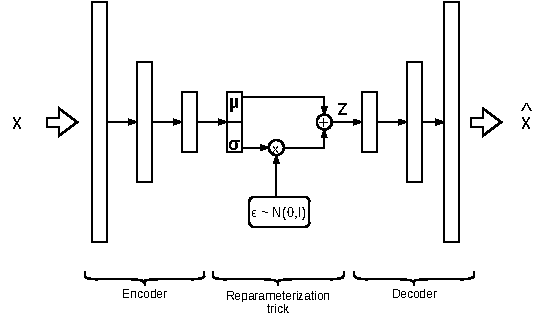
\includegraphics[width=1\linewidth]{background/images/vae}
	\caption[\textit{Variational auto-encoder}]{Diagram showing how a \textit{variational auto-encoder} is structured. }
	\label{fig:vae}
\end{figure}

A known probability distribution $q$ with parameters $\phi$ will be used to approximate $p$ so that $q_\phi(\mathbf{z}|\mathbf{x}) \approx p_\mathbf{\theta}(\mathbf{z}|\mathbf{x})$. For that, the \textit{Kullback-Leibler} divergence ($D_{KL}$) metric will be used to minimize the differences between the two distributions, as shown in equation \ref{eq:dklvae} \autocite{kingma2019}. $\mathcal{L}(\mathbf{x}, \mathbf{\theta}, \phi)$, from equation \ref{eq:lbvae}, represents a lower bound (often referred as evidence lower bound, \textit{ELBO}, or negative free energy), given that $D_{K L}\left(q_{\phi}(\mathbf{z} \mid \mathbf{x}) \| p_{\mathbf{\theta}}(\mathbf{z} \mid \mathbf{x})\right)$ is always greater or equal to zero (see the optimization function in equation \ref{eq:vaelbasloss}). As the lower bound is tractable, the optimization problem can be approximated as shown in equation \ref{eq:vaeopt}. In other words, maximizing the lower bound assures that the log-likelihood of the data is at least as large as its lower bound \autocite{wei2021}.

\begin{equation}
\label{eq:dklvae}
\min_{\phi} D_{KL}\left(q_\phi(\mathbf{z}|\mathbf{x}), p_\mathbf{\theta}(\mathbf{z}|\mathbf{x})\right)
\end{equation}

\begin{equation}
\label{eq:lbvae}
\begin{aligned}
\log \left(p_{\mathbf{\theta}}(\mathbf{x})\right) =& \underbrace{D_{K L}\left(q_{\phi}(\mathbf{z} \mid \mathbf{x}) \| p_{\mathbf{\theta}}(\mathbf{z} \mid \mathbf{x})\right)}_{>0} \ldots \\
&+\underbrace{\mathbb{E}_{\mathbf{z}} \log p_{\mathbf{\theta}}(\mathbf{x} \mid \mathbf{z})-D_{K L}\left(q_{\phi}(\mathbf{z} \mid \mathbf{x}) \| p_{\mathbf{\theta}}(\mathbf{z})\right)}_{\mathcal{L}(\mathbf{x}, \mathbf{\theta}, \phi)}
\end{aligned}
\end{equation}

\begin{equation}
\label{eq:vaelbasloss}
\log p_{0}(\mathbf{x}) \geq \mathcal{L}_{\mathbf{\theta}, \phi}\left(\mathbf{x}\right)
\end{equation}

\begin{equation}
\label{eq:vaeopt}
\mathbf{\theta}, \phi \leftarrow \underset{\mathbf{\theta}, \phi}{\arg \max } \sum_{i=1}^{N}\left(\mathcal{L}_{\mathbf{\theta}, \phi}(\mathbf{x})\right)
\end{equation}

The first term of the lower bound of equation \ref{eq:lbvae} ($\mathbb{E}_{\mathbf{z}} \log p_{\mathbf{\theta}}(\mathbf{x} \mid \mathbf{z})$) is known as the reconstruction error, and measures how dissimilar the input and the output are. The second term ($D_{K L}\left(q_{\phi}(\mathbf{z} \mid \mathbf{x}) \| p_{\mathbf{\theta}}(\mathbf{z})\right)$), usually referred as the divergence error, measures how dissimilar are the prior and the posterior distributions of the encoder. The probability distributions $p_\mathbf{\theta}$ and $q_\phi$ are two separated deep learning models (with parameter sets $\mathbf{\theta}$ and $\phi$). Normally, the prior distribution over the latent variables $P(\mathbf{z})$ is chosen to be an \textit{isotropic Gaussian} \autocite{wei2021} and in order to ensure that the encoder-decoder architecture is differentiable everywhere, the \textit{re-parameterization trick} is used as a mechanism to replace the classical non-differentiable sampling procedure $\mathbf{z} \sim N(\mathbf{\mu}, \mathbf{\sigma})$ by an equivalent version $\mathbf{z} = \mathbf{\mu} + \epsilon \cdot \mathbf{\sigma}$ where $\epsilon \sim N(0,I)$, in which $z$ is differentiable with respect to $\mathbf{\mu}$ and $\mathbf{\sigma}$ \autocite{kingma2019}.


\subsubsection{Generative adversarial networks}
\textit{Generative adversarial networks} (GAN hereafter) are a type of deep generative models first published in 2014 \autocite{Goodfellow2014}. They consist of a dual deep learning model, where the first component, known as the generator, tries to generate realistic data samples, and the discriminator (the generator's adversary) attempts to determine if a given sample is real or generated. As an analogy, one can think of the generator as playing the role of a counterfeiter, and the discriminator playing the role of a police officer. The role of the counterfeiter is to try to fool the police officer, while the latter will try to catch the counterfeiter. Figure \ref{fig:police_counterfeiter} shows this process graphically.

The training process of a GAN is generally a zero-sum game, where the optimization succeeds when the system reaches the \textit{Nash} equilibrium \autocite{nash48}. The goal of the algorithm is to learn to represent an estimated distribution ($p_{\mathrm{model}}$) of a given data distribution ($p_{\mathrm{data}}$). Moreover, GANs are designed to be unbiased \autocite{Goodfellow2016}, in the sense that provided with enough data, a model with enough capacity and the proper learning algorithm, the true probability distribution of the data can be perfectly recovered: $p_{\mathrm{model}} = p_{\mathrm{data}}$. As an important practical aspect of GANs, once the algorithm has converged the generator is able to synthesize samples of $p_\mathrm{model}$, however the learned probability density function (PDF) is implicit. GANs provide no access to the learned PDF.

In the GAN systems, the generator $f_g$ is a deep learning model with parameters $\mathbf{\theta^g}$ that takes a latent vector $\mathbf{z} \sim p(\mathbf{z})$ as input, where $p$ is a prior distribution (usually chosen to be a \textit{Gaussian} distribution), and produces a sample $\hat{\mathbf{x}}=f_g(\mathbf{z})$. The discriminator $f_d$ is another deep learning model with parameters $\mathbf{\theta^d}$ that takes a sample $\mathbf{x}$ as input, and produces a binary output $f_d(\mathbf{x})$ that models the probability of the input sample $\mathbf{x}$ being real or generated \autocite{Goodfellow2014}. In this setting, the GAN objective can be formulated as a \textit{minimax} objective, as shown in equation \ref{eq:ganminimax}. The default loss function (represented as $J$), is defined in equation \ref{eq:ganloss}. Unfortunately, the training objective is non-convex in $\theta^g$ and $\theta^d$, which makes training difficult when using complex neural networks, often leading to underfitted models \autocite{Goodfellow2016b,Goodfellow2016}. In a simpler manner, when one of the two networks becomes too strong, the system diverges. Stabilization of the GANs remains an open problem, although some advances have been recently made \autocite{arjovsky2017, shaobo2017, wang2022}.

\begin{equation}
	\label{eq:ganminimax}
	f_g^*, f_d^* = \arg \min_{\theta_g} \max_{\theta_d} J(f_g, f_d)
\end{equation}

\begin{equation}
	\label{eq:ganloss}
	J(\theta^g, \theta^d) = \mathbb{E}_{\mathbf{x}\sim p_\mathrm{data}} \log (f_d(\mathbf{x})) + \mathbb{E}_{\mathbf{x}\sim p_{model}} \log (1 - f_d(\mathbf{x}))
\end{equation}

The generator and discriminator models must be differentiable everywhere, otherwise the model cannot be trained with backpropagation. As an important detail that can be noticed in equation \ref{eq:ganminimax}, both players have a cost function (equation \ref{eq:ganloss}) that depends on the superset  of parameters $\{\theta^g, \theta^d\}$, but every player can only change its own parameters, and not the adversary's.

\begin{figure}[h!]
	\centering
	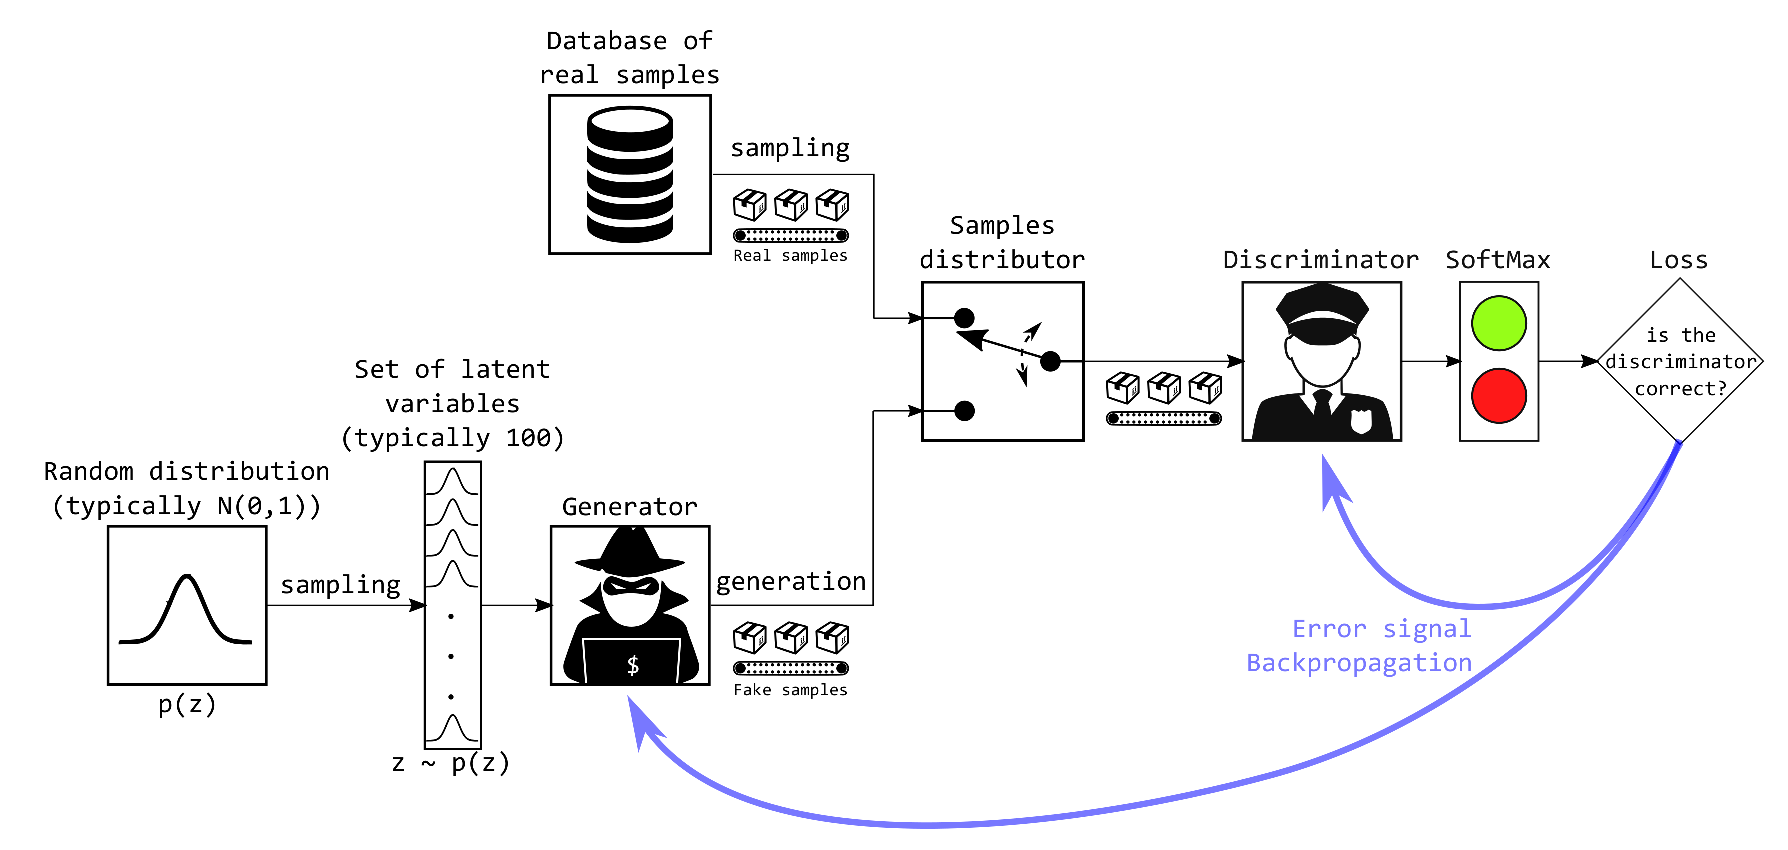
\includegraphics[width=1\textwidth]{background/images/police_counterfeiter.eps}
	\caption[Generative adversarial network]{\textit{Generative adversarial network} diagram, showing the role of the generator and the discriminator and the error signals backpropagated through the network.}
	\label{fig:police_counterfeiter}
\end{figure}

\subsubsection{Normalizing flows} \label{sec:flows}
\textit{Normalizing Flows} are another type of deep generative models that are used to approximate data distributions $p_\mathrm{data}$. These models describe the transformation of a prior density function $p(z)$ into an arbitrarily complex probability distribution $p_\mathrm{model}$, through a series of invertible mappings, by repeatedly applying the rule for change of variables \autocite{rezende2015}. The output of the series of invertible functions applied to the prior distribution is still a valid probability distribution, and hence this type of models is known as normalizing flow.

A flow $f: \mathbb{R}^d \rightarrow \mathbb{R}^d$ is an invertible mapping (i.e. $\exists f^{-1}$) such that given a random variable $\mathbf{x} \sim p(\mathbf{x})$, then $f(f^{-1}(\mathbf{x})) = \mathbf{x}$. The probability density function $p(\mathbf{x})$ could be approximated by applying the rule for change of variables, as shown in equation \ref{eq:flowcov}, where $p(z)$ is known. Notice that the right hand side of the  equation \ref{eq:flowcov} comes from the application of the inverse function theorem \autocite{rezende2015}.

Invertible and differentiable flows are closed under composition \autocite{kobyzev}. This means that when composing multiple flows, the resulting function is still a flow. That property is very important for building deep normalizing flows capable of modeling complex data distributions such as images. It can be easily seen from equation \ref{eq:flowcov}  \autocite{rezende2015} that given a composition of $F$ flows $\mathbf{x}=f_F \circ ... f_1(\mathbf{z})$, the probability distribution $p_F(\mathbf{z_F})$ can be easily obtained through the application of the change of variables formula, as shown in equation \ref{eq:flowcovcomp} (expressed as log-probability for mathematical convenience), where $h_k$ is the output vector of the flow $f_k$.


\begin{equation}
\label{eq:flowcov}
p_\theta(\mathbf{x}) = p_\theta(f^{-1}(\mathbf{x})) \cdot \left| \det \frac{\partial f^{-1}(\mathbf{x})}{\partial \mathbf{x}} \right| = p(\mathbf{z}) \cdot \left| \det \frac{\partial f(z)}{\partial \mathbf{z}} \right|^{-1}
\end{equation}


\begin{equation}
\label{eq:flowcovcomp}
\log p_\theta(\mathbf{x}) 
= \log p_\theta(\mathbf{z}) + \log  \left| \det \frac{\partial \mathbf{z}}{\partial \mathbf{x}} \right| 
= \log p_\theta(\mathbf{z}) + \sum_{k=1}^{F} \log  \left| \det \frac{\partial \mathbf{h}_k}{\partial \mathbf{h}_{k-1}} \right| 
\end{equation}


The normalizing flow is trained by maximizing the PDF of the samples $\mathbf{x}$, which can be calculated as the probability density of the normalized samples $p(f^{-1}(\mathbf{x}))$ with a volume correction term derived from the change of variables formula, as expressed in \ref{eq:flowcovcomp} \autocite{papamakarios2017}. Once the model is trained, one can sample from the prior distribution $\mathbf{z} \sim p(\mathbf{z})$ and transform that latent variable into a data sample $\hat{\mathbf{x}} = f(\mathbf{z})$ \autocite{rezende2015}.

There are two main restrictions that have to be taken into account when designing neural architectures for normalizing flows. First, each flow block $f_i$ needs to be invertible, and second, the determinant of the \textit{Jacobian} of each flow block must be fast to compute. These two properties are absolutely necessary for being able to train deep learning based normalizing flows, and they represent the major difficulty currently under research. The most common solution at the time of writing this dissertation is to define the flows $f_i$ as affine-coupling layers \autocite{dinh2018}. Their structure is represented in figure \ref{fig:affinecouplingblock}. More formally, given an input vector $\mathbf{x}$, of size $\mathbf{D}$, an integer $d \in [2,D-1]$, a deep learning model $s$ and another $l$, the affine-coupling layers can be defined as shown in equation \ref{eq:affinecouplingblock}. It can be shown that the determinant of the \textit{Jacobian} of the affine-coupling layer transformation does not depend on the parameters of the networks $l$ and $s$, so they can be as complex as one wants \autocite{dinh2018}. The whole operation can be seen as a scale and shift operation applied over one part of the input vector $\mathbf{x_{d+1:D}}$, and conditioned over the other $\mathbf{x_{1:d}}$. The composition of multiple affine-coupling layers with interleaved shuffling operations builds \textit{RealNVP} \autocite{dinh2018}, a deep normalizing flow that achieved remarkable results in computer vision.

\begin{equation}
\label{eq:affinecouplingblock}
\begin{gathered}
	 \mathbf{y} = \begin{cases} \mathbf{y_{1: d}} & = \mathbf{x_{1: d}} \\
	\mathbf{y_{d+1: D}} & =\mathbf{x_{d+1: D}} \odot s\left(\mathbf{x_{1: d}}\right)+l\left(\mathbf{x_{1: d}}\right)\end{cases} \\
	\mathbf{x} = \begin{cases}
	\mathbf{x_{1: d}} &=\mathbf{y_{1: d}} \\
	\mathbf{x_{d+1: D}} &=\left(\mathbf{y_{d+1: D}}-l\left(\mathbf{y_{1: d}}\right)\right) \odot s\left(\mathbf{y_{1: d}}\right)
	\end{cases}
\end{gathered}
\end{equation}

\begin{figure}[h!]
	\centering
	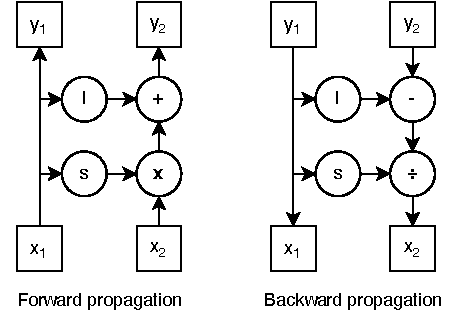
\includegraphics[width=0.5\linewidth]{background/images/affinecouplingblock}
	\caption[Normalizing flows affine coupling layers]{Forward and backward computation graphs for \textit{affine-coupling layers}. Notice that $\mathbf{x_1}$ and $\mathbf{x_2}$ represent the input vector $\mathbf{x}$ split in two parts, and the affine coupling operation produces two vectors $\mathbf{y_1}$ and $\mathbf{y_2}$ of the exact same size as $\mathbf{x_1}$ and $\mathbf{x_2}$, respectively. The nodes with the letters $l$ and $s$ are arbitrarily complex neural networks that, conditioned to the first vector, produce scaling and translation weights to be applied over the second vector.}
	\label{fig:affinecouplingblock}
\end{figure}


Other common solutions to the same problem are known as masked auto-regressive flows \autocite{papamakarios2017}, inverse auto-regressive flows \autocite{kingma2016} or \textit{glow} \autocite{kingma2018}. They will not be covered here because it is out of the scope of this dissertation. More details about \textit{glow} will be given in chapter \ref{ch:tts}.


\subsubsection{Evaluation} \label{sec:dgmevaluation}
One of the most important aspects of any discipline in science is the ability to properly measure the phenomenon under study, and the field of generative models is not an exception. However, measuring how well a generative model performs can be an extremely difficult task \autocite{Goodfellow2016}. There are several approximate approaches that aim to quantify the performance of a generator \autocite{theis2016a}, but we still do not have a general way to tackle this problem.

Many of the applications of generative models deal with multimedia data such as images, music, speech, etc. Our way of determining if a set of synthetic media has good or bad quality is through perceptual judgement. Generative models can be evaluated using perceptual judgement, but as any type of judgement, it may be subject to biases. To avoid a biased evaluation, the evaluation set and the jury needs to be carefully chosen. Even if these pieces are designed carefully, there is still risk that this subjective evaluation completely fails \autocite{Goodfellow2016}. One possible case is the hypothetical example in which a model learns to memorize the training data. In that case, the model will not be succeeding at the generation task, but a perceptual test would score the model with very high performance. Other example could be a model which is collapsed into a mode in the data. For example, given a model that is trained to generate images of cats and dogs, if the model only learns to generate high quality images of cats and never generates dogs', it may get a high score out of a subjective test, while it is completely failing to capture the variability of the data. For these reasons, it is well known that subjective quality of samples is not a reliable way of evaluating generative models \autocite{denton2015}.

Other common way to evaluate generative models consists of measuring the log-likelihood of the $p_\mathrm{model}$ over a test set, in the cases in which the log-likelihood is tractable \autocite{Goodfellow2016}. This approach may be informative in some cases, but it is not a solution at all, as it often may not be correlated with the perceptual quality. One example could be a speech synthesis model that models the silences in the recordings with a very small variance. The probability density in those regions would be extremely high, while perceptually we would not probably be interested on accurately reproducing background noise. Additionally, the comparison of log-likelihoods of different models should be done under the same conditions. Aspects like data processing, the type of algorithm that is used to approximate the log-likelihood or the choice of the prior distribution can bias the results \autocite{Goodfellow2016}.

This topic is still an open research problem, and many studies have already provided some insights about it \autocite{theis2016a, sajjadi2018}. However, the problem remains still unsolved.




%!TEX root = ../thesis.tex
\chapter{The modulus as activation function} \label{ch:modulus}

\section{Overview}
The idea of decreasing the size of neural networks has been studied since long time ago \autocite{lecun1989, hassibi1993, frankleC19}. Many applications may require to be efficient at training or at inference times, especially the models that need to be executed on mobile and embedded devices \autocite{ooko2021, zapico2021}. One of the most impressive examples is the wake word detection system of the \textit{Google} assistant, which was reported to weight only 14 kilobytes in size \autocite{warden2020}. 

The subfield of machine learning that researches how to minimize the computational cost is commonly known as \textit{TinyML} \autocite{han2022}. \textit{TinyML} not only brings obvious energy consumption benefits but it can also be used to reduce the latency of the response of such systems because the devices would no longer need to query large cloud servers, removing the dependency on internet connections and allowing them to work offline. Furthermore, the common privacy concerns of machine learning applications \autocite{ha2019} can be easily diluted if all the sensible data collected are processed solely into the device, and never leaves home.

This chapter introduces a new non-monotonic activation function --the \textit{modulus}-- which simplicity makes it specially suitable for \textit{TinyML} and other low resource applications: the modulus and its derivative are simply bit-size operations. Interestingly, the gradient norm does not depend on the input, which removes some of the problems reported on other nonlinearities \autocite{lu2020, pascanu13, hochreiter1998, Hochreiter2001}. The experiment results provide evidence that when using the \textit{modulus} activation function on computer vision tasks the models generalize better than with other nonlinearities - up to a 15\% accuracy increase in \textit{CIFAR100} dataset and 4\% in \textit{CIFAR10} dataset (with respect to the benchmark activations tested). 



The code used along this work has been made available in a public repository\footnote{\url{https://github.com/ivallesp/abs}}.


\section{Introduction}
As discussed in section \ref{sec:mlp}, the core piece of all deep learning models is the activation function. They enable the models to produce non-linear abstract representations when applying linear transformations in cascade \autocite{Goodfellow2016}. The most common choice in modern deep learning models is the Rectified Linear Unit (\textit{ReLU}) \autocite{nair2010}. Among other advantages, \textit{ReLU} nonlinearities allow to train deeper neural networks \autocite{xu2015}.

\section{Previous work}
Apart from the \textit{ReLU} in the last years there have appeared many alternative activation functions. The following studies represent some of the most popular examples: \textit{Leaky-ReLU} and \textit{PR-ReLU} \autocite{xu2015}, \textit{ELU} \autocite{djork2016}, \textit{Swish} \autocite{ramachandran2018}, \textit{SELU} \autocite{klambauer2017}, \textit{F/PFLU} \autocite{zhu2020}, \textit{RSigElu} \autocite{Kilicarslan2021} etc. All those activation functions have the following properties in common: nonlinearity, continuity, differentiability and low computational cost (being \textit{Swish} the most computationally expensive option). The majority of the activation functions are monotonic, \textit{Swish} \autocite{ramachandran2018}, \textit{GELU} \autocite{hendrycks2016},  \textit{S-ReLU} \autocite{Jin2016} and \textit{Mish} \autocite{misra2019mish} are some of the most popular modern exceptions. Despite the large pool of alternatives, \textit{ReLU} still appears as the default choice in many applications due to its simplicity and low computational cost \autocite{nair2010}.

This chapter delves into the world of the non-monotonic nonlinearities and proposes the \textit{modulus} function (aka absolute value) as an activation function, providing empirical evidences  proving that this activation function allows deep learning models to converge to better solutions in \textit{CIFAR10}, \textit{CIFAR100} and \textit{MNIST} datasets. 

Compared with other modern non-monotonic nonlinearities such as \textit{Mish} \autocite{misra2019mish}, \textit{PFLU} and \textit{FPFLU} \autocite{zhu2020} or \textit{Swish}  \autocite{ramachandran2018}, the \textit{modulus} has a very low computational cost (equivalent to \textit{ReLU}). This property makes the \textit{modulus} specially useful for \textit{TinyML} \autocite{sanchez2020} and hardware \autocite{Misra2010} applications.

%The contributions of this work are: (1) proposal of the modulus as activation function, (2) the proposed function empirically shows significantly superior results in 75\% of our experiments, (3) we- contribute to the new trend of non-monotonic activation functions with another example showing results in the same direction, (4) the simplicity of the modulus activation function makes it very suitable for hardware applications and \textit{TinyML}, and (5) we- propose two smooth approximation to the \textit{modulus} function, one of them achieving even superior results than the original \textit{modulus}.

%This chapter is organized as follows. Section \ref{sec:modulus_methods} describes the proposed activation function and the ones used for benchmarking. Section \ref{sec:modulus_experiments} describes the experiments conducted and the results achieved. Finally, we- summarize our contribution in section \ref{sec:modulus_conclusions}, enumerating the main conclusions.


% Ideas
% Non-dying regions

\section{Methods} \label{sec:modulus_methods}
\subsection{Modulus activation function}
This section introduces the proposed activation function, the \textit{modulus}: $f(x)=|x|$. This nonlinearity is a continuous, piecewise-linear function consisting of an identity mapping for positive values of $x$, and a negative identity mapping for negative values of $x$. Its derivative (defined below) as well as the modulus function itself, are bit-size operations. This is extremely useful for hardware implementations. Besides, the modulus function can be expressed as $f(x) = \text{sgn}(x)\cdot x$, where $f'(x) = \text{sgn}(x)$. In practice, this means that the derivative can be calculated as part of the forward pass and cached for the \textit{backpropagation}, reducing the total computation. This form is also specially useful in hardware implementations, given that the whole activation function is fully represented as a bit-size operation (the sign function).

$$
f'(x)= \left\{ \begin{array}{lcc}
1 &   \text{if}  & x > 0 \\
-1 &  \text{if} & x < 0
\end{array} \right.
$$

Notice that the \textit{modulus} function is differentiable everywhere except in $x = 0$. For practical purposes,  $f'(0) := 1$  so that the derivative is defined for all the range of $x$ values, similar to the case of \textit{ReLU} \autocite{Goodfellow2016}. See figure \ref{fig:activations}h for a graphical representation.


The \textit{modulus} activation function belongs, in essence, to the family of rectifier functions \autocite{glorot2015} . In fact, it is equivalent to a \textit{Leaky-ReLU} with $\alpha=-1$. However \textit{Leaky-ReLU} was originally defined to take values of alpha strictly higher than 0 \autocite{xu2015}. Furthermore, \textit{modulus} achieves significantly superior results than the \textit{Leaky-ReLU}.

\begin{figure}[h!]
	\centering
	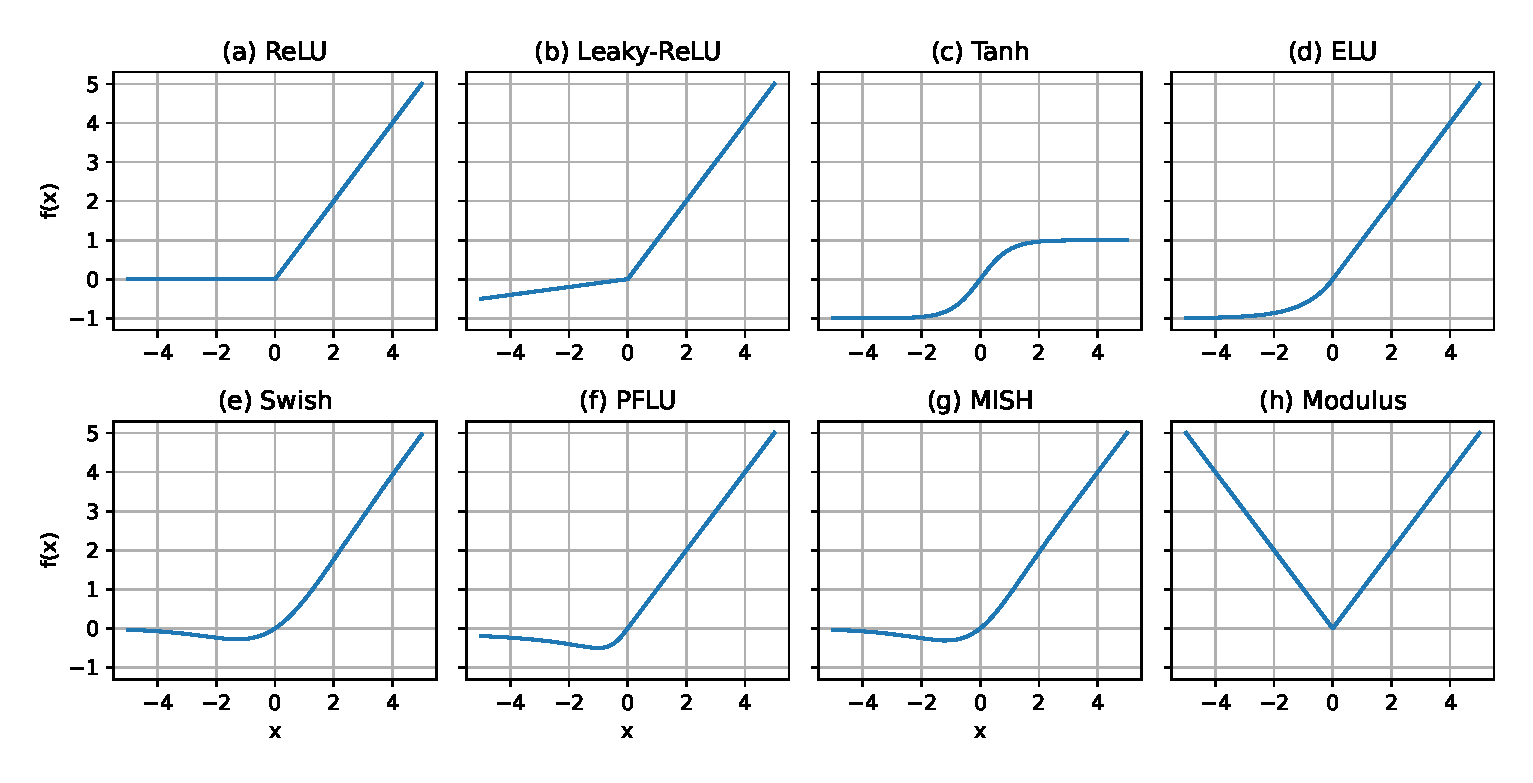
\includegraphics[width=1.0\linewidth]{modulus/images/activations}
	\caption{Nonlinearities used along this study. (a-g) are benchmark activation functions that showed good performance in previous studies. (h) is the \textit{modulus} activation function proposed in this chapter. For this example, the default hyper-parameters have been used for the \textit{Leaky-ReLU}, \textit{ELU} and \textit{Swish} activation functions, respectively.
	}
	\label{fig:activations}
\end{figure}

The benefit of this activation function with respect to the other rectifiers is that the norm of its gradient is constant ($||\nabla_x f|| = 1 \quad \forall x$) and hence it does not depend on the input value. This property is desirable when optimizing the parameters of a neural network with gradient descent algorithms, as there are no input values for which the neuron saturates \autocite{glorot2010} (i.e. values of x for which the gradient of the activation function is close to zero). This naturally removes the dying neurons \autocite{lu2020} and vanishing gradient problems \autocite{pascanu13, hochreiter1998, Hochreiter2001}.

\subsection{Smooth approximations of the modulus function}
The \textit{modulus} function is not differentiable when $x=0$. To study if this property harms the performance of the models in any way, two alternative smooth approximations of the \textit{modulus} function have been tested as an additional experiment. See figure \ref{fig:activationssmooth} for a visual representation. The two approximations are defined below.


\begin{figure}[h!]
	\centering
	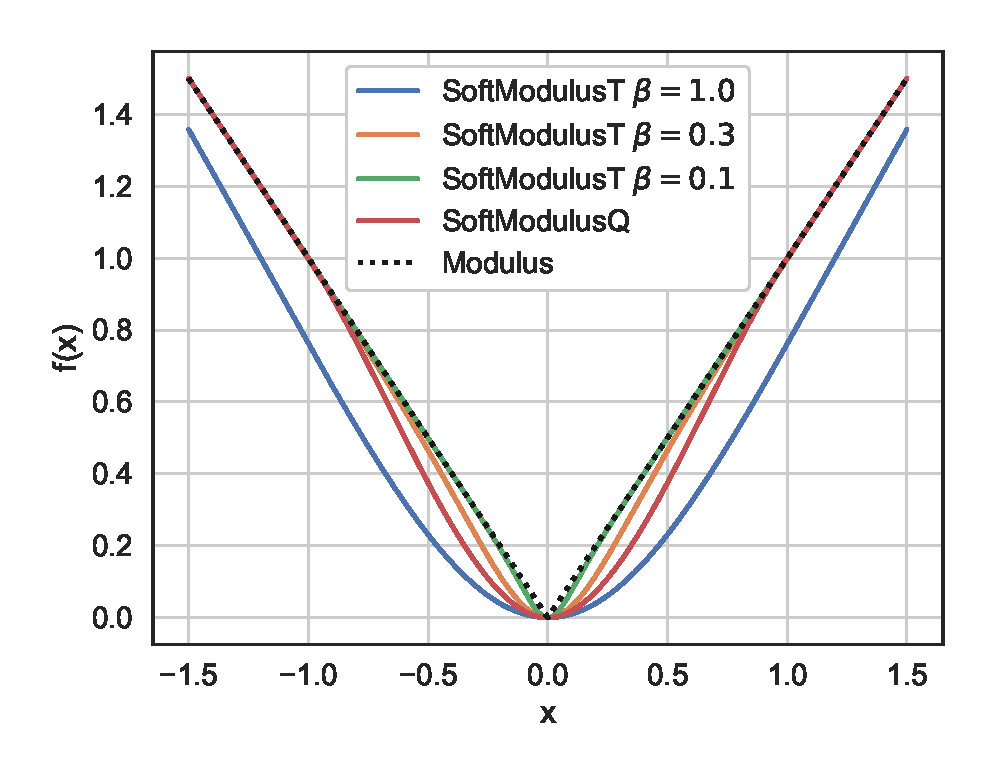
\includegraphics[width=0.5\linewidth]{modulus/images/activations_smooth}
	\caption{Representation of the two \textit{SoftModulus} activation functions compared with the original \textit{modulus}: \textit{SoftModulusQ} and \textit{SoftModulusT}.}
	\label{fig:activationssmooth}
\end{figure}


\subsubsection{Quadratic approximation}
A fuzzy set approach is chosen as a method to combine the modulus function with a quadratic function (see figure \ref{fig:fuzzy_funcs}) to get a smooth approximation. For that, three membership functions are defined in figure \ref{fig:fuzzy} and equations \ref{eq:mulow}, \ref{eq:mumid}, \ref{eq:muhigh}.

\begin{figure}[h!]
	\centering
	\includegraphics[width=0.7\linewidth]{modulus/images/funcs_quad}
	\caption{Quadratic and modulus functions, together with the combined one (in blue, red and green, respectively).}
	\label{fig:fuzzy_funcs}
\end{figure}

\begin{figure}[h!]
	\centering
	\includegraphics[width=0.7\linewidth]{modulus/images/fuzzy}
	\caption{Membership functions used to combine the quadratic and modulus functions.)}
	\label{fig:fuzzy}
\end{figure}

\begin{equation}
\label{eq:mulow}
\mu^x_{\text{low}}= \left\{ \begin{array}{lcc}
1 &   \text{if}  & x < -1 \\
-x & \text{if}  & -1 \leq x < 0 \\
0 &  \text{if} & x \geq 0
\end{array}
\right.
\end{equation}

\begin{equation}
\label{eq:mumid}
\mu^x_{\text{med}}= \left\{ \begin{array}{lcc}
0 &   \text{if}  & x < -1 \\
x+1 & \text{if}  & -1 \leq x < 0 \\
1-x & \text{if}  & 0 \leq x < 1 \\
0 &  \text{if} & x \geq 1
\end{array}
\right.
\end{equation}

\begin{equation}
\label{eq:muhigh}
\mu^x_{\text{high}}= \left\{ \begin{array}{lcc}
0 &   \text{if}  & x < 0 \\
x & \text{if}  & 0 \leq x < 1 \\
1 &  \text{if} & x \geq 1
\end{array}
\right.
\end{equation}

Let $f^x_{\text{low}}=-x$, $f^x_{\text{med}}=x^2$ and $f^x_{\text{high}}=x$. These functions are combined with the membership functions to get the quadratic approximation.

\begin{itemize}
	\item For $x < -1$:  $\hat{f}(x)=\frac{f^x_{\text{low}} \cdot \mu^x_{\text{low}}}{\mu^x_{\text{low}}}=-x$

	\item For $-1\leq x < 0$:  $\hat{f}(x)=\frac{f^x_{\text{low}} \cdot \mu^x_{\text{low}} + f^x_{\text{med}} \cdot \mu^x_{\text{med}}}{\mu^x_{\text{low}} + \mu^x_{\text{med}}}=\frac{(x+1)x^2+(-x)(-x)}{1+x-x}=x^3 + 2x^2$

	\item For $0\leq x < 1$:  $\hat{f}(x)=\frac{f^x_{\text{med}} \cdot \mu^x_{\text{med}} + f^x_{\text{high}} \cdot \mu^x_{\text{high}}}{\mu^x_{\text{med}} + \mu^x_{\text{high}}}=\frac{(1-x)x^2+x\cdot x}{1-x+x}=-x^3 + 2x^2$

	\item For $x \geq 1$:  $\hat{f}(x)=\frac{f^x_{\text{high}} \cdot \mu^x_{\text{high}}}{\mu^x_{\text{high}}}=x$
\end{itemize}

Combining and simplifying all the above expressions the final activation function is obtained. This approximation is subsequently referred as \textit{SoftModulusQ}.


$$
f(x)= \left\{ \begin{array}{lcc}
x^2 \cdot (2-|x|) &  \text{if} & |x| \leq 1 \\
|x| &   \text{if}  & |x| > 1
\end{array}
\right.
$$


\subsubsection{Hyperbolic tangent approximation}
Starting from the modulus function $f(x)=sgn(x)\cdot x$, the $sgn$ function is approximated as follows $sgn(x) \approx \tanh(x/\beta)$, where $\beta \in [0, 1]$ is a tunable hyperparameter that controls how acute the ``V'' transition is. The smaller the $\beta$, the closest the approximation is to the \textit{modulus}. A value of $\beta=0.01$ is used along all the trained models. In the rest of the chapter, this approximation is referred as \textit{SoftModulusT}.

	$$f(x) = x \cdot \tanh(x/\beta)$$



% TODO: \usepackage{graphicx} required

\subsection{Benchmark activation functions}
The following activation functions have been used as a benchmark to compare the performance of the proposed one.


\begin{itemize}
	\item \textit{Tanh}: the hyperbolic tangent has been one of the most popular choices (together with the \textit{sigmoid}), before \textit{ReLU} was proposed \autocite{lecun2012}. Among many other desirable properties, its derivative is very simple: $(\tanh x)'=1-\tanh^2 x$. This property was very beneficial specially before automatic differentiation tools appeared. Besides, similar to the proposed activation function, the derivative can be easily calculated during forward pass and cached for the backward pass.
	\item \textit{ReLU}: this activation function was published in 2010 as an alternative to train \textit{Restricted Boltzman Machines} \autocite{nair2010}. It is defined as $f(x) = \max(0,x)$. It allowed training deeper neural networks by solving the vanishing gradient problems typically happening with saturating activation functions. As it can be seen in the formula, ReLU outputs zero if the input is negative. This brings sparsity to the non-linear representation, at the cost of potentially finding optimization problems due to the fact that the derivative when $x<0$ is zero (dying neurons, for instance).
	\item \textit{Leaky-ReLU}: the \textit{Leaky-ReLU} \autocite{xu2015} attempted to solve the problem known as \textit{dying neurons} in the \textit{ReLUs} by adding a small linear term in the negative side of $x$: $f(x) = \max(x/\beta, x)$, where $\beta$ is a hyperparameter to be tuned: $\beta>1$ and $\sigma$ is the logistic function.
	\item \textit{ELU}: this is a smooth version of \textit{ReLU} \autocite{djork2016} that approaches asymptotically to -1 when $x=-\inf$. Unlike ReLUs, it is differentiable everywhere and can produce negative values. This activation function is formally defined as follows. $\alpha$ is a tunable hyperparameter.
	$$
	f(x)= \left\{ \begin{array}{lcc}
		x &   \text{if}  & x > 0 \\
 \alpha(e^x - 1) &  \text{if} & x \leq 0
	\end{array}
	\right.
	$$

	\item \textit{Swish}: this is one of the few non-monotonic activation functions formally published \autocite{ramachandran2018}. It is defined as $f(x) = x \cdot \sigma(\beta x)$, where $\beta$ is a hyperparameter to be tuned. It gained its popularity by showing promising results in multiple applications. 
	\item \textit{Mish}: this is a smooth, non-monotonic and self-regularized activation function, similar to \textit{Swish}, showing superior performance in different benchmarks \autocite{misra2019mish}. It is defined as $f(x) = x \tanh \left[\text{softplus} (x)\right]$, where $\text{softplus} (x) = \log(1+e^x)$ \autocite{dugas2001}.
	\item \textit{PFLU}: the Power Function Linear Unit (PFLU) is a non-monotonic activation function that showed good performance in convolutional architectures \autocite{zhu2020}. It is defined as follows: $f(x) = x \cdot \frac{1}{2} \left( 1 + \frac{x}{\sqrt{1+x^2}} \right)$.

\end{itemize}

\section{Experiments and results} \label{sec:modulus_experiments}
\subsection{Setup}



For the following experiments, \textit{CIFAR10}, \textit{CIFAR100} \autocite{krizhevsky09} and \textit{MNIST} \autocite{lecun2010} datasets have been used. \textit{CIFAR10} and \textit{CIFAR100} images are labeled into 10 and 100 classes, respectively. They are of size 32x32 and full color. 

In both cases, the datasets contain 50,000 images for training and 10,000 images for testing purposes. \textit{MNIST} images belong to one of 10 classes and are in grey scale and 28x28 size. \textit{MNIST} comes with 50,000 images for training and 10,000 images for testing purposes.

The images of the datasets have been normalized so that the minimum and the maximum values are -1 and 1. 

Four different architectures have been used to test the performance of the \textit{modulus} activation function against the other nonlinearities. These architectures, described in Table \ref{tab:architectures}, are inspired on the ones used in the \textit{Lottery Ticket Hypothesis} study \autocite{frankleC19}.


\begin{table}[h] \small
	\caption{Deep learning architectures used to experiment with different activations. In the dense layers row, the output size has been represented as $C$. The Fully connected architecture (\textit{FC}) is a multilayer perceptron with 2 hidden layers + the output layer. The \textit{Conv2} and \textit{Conv6} architectures are shallow variants of \textit{VGG} described here: \autocite{simonyan2015}. The last pooling layer of the \textit{VGG-16} original architecture has been trimmed in order to allow this model to work with smaller image sizes.}
	\setcellgapes{3pt}\makegapedcells
	\begin{tabular}[t]{lllll}
		\toprule
		Network              & Fully Connected & Conv2       & Conv6                                                & VGG-16                                                                                  \\ \midrule
		\makecell[l]{Conv layers\\\\\\\\\\} &                & \makecell[l]{64,64,pool\\\\\\\\\\}  & \makecell[l]{64,64,pool\\128,128,pool\\256,256,pool\\\\\\} & \makecell[l]{64,64,pool\\128,128,pool\\256,256,256,pool\\512,512,512,pool\\512,512,512} \\
		Dense Layers         & 256,256,$C$     & 256,256,$C$ & 256,256,$C$                                          & 4096,4096,$C$                                                                           \\
		Filter sizes &  & 3x3 & 3x3 & 3x3 \\
		Pooling type & & max & max & max \\
		\# Parameters        & 269k-878k       & 3.3M-4.3M   & 1.8M-2.3M                                            & 33.6M-40.3M                                                                             \\
		Size                 & 3.1-11MB & 38-50MB & 21-27MB & 385-462MB \\ \bottomrule
	\end{tabular}
	\label{tab:architectures}
	\vspace{20pt}
\end{table}


\definecolor{First}{HTML}{A2BEFF}
\definecolor{Second}{HTML}{A8FFD4}
\definecolor{Third}{HTML}{FFEDB8}
\definecolor{Fourth}{HTML}{FFB8C8}


\begin{table}[h!] \footnotesize  \setlength{\tabcolsep}{3pt}
	\caption{Classification accuracy for all the datasets and activation functions tested (rows), and for all the models (columns). The results are expressed as mean $\pm$ standard deviation across the 30 random initializations. To facilitate the reading of the table, for each dataset-model combination, the results have been colored as follows: the best result (highest accuracy) has been colored in blue, the second in green, the third in yellow and the fourth in red (\colorbox{First}{first} $>$ \colorbox{Second}{second} $>$ \colorbox{Third}{third} $>$ \colorbox{Fourth}{fourth}). Additionally, the cases where any of the proposed activation functions achieved significantly higher accuracy (with a significance level of $\alpha=0.05$) than the benchmarks is marked in bold. A \textit{Wilcoxon one-sided Rank Sum} test has been used to quantify the statistical significance.}
	\centering
	\begin{tabular}{rrcccc}
		\toprule
		 Dataset &   Activation &                     FC                      &                    Conv2                    &                    Conv6                    &                    VGG16                    \\ \midrule
		 CIFAR10 &         ReLU &              $54.65 \pm 0.22$               &              $71.40 \pm 0.26$               &              $77.09 \pm 1.21$               &     $\cellcolor{Fourth}83.66 \pm 0.41$      \\
		         &    LeakyReLU &              $54.71 \pm 0.24$               &      $\cellcolor{Third}71.65 \pm 0.32$      &              $77.38 \pm 1.13$               &      $\cellcolor{Third}83.98 \pm 0.34$      \\
		         &         Tanh &              $49.95 \pm 0.23$               &              $67.46 \pm 0.34$               &              $77.67 \pm 0.24$               &              $79.69 \pm 0.26$               \\
		         &        Swish &      $\cellcolor{Third}55.39 \pm 0.29$      &              $69.09 \pm 0.27$               &              $71.66 \pm 0.62$               &              $80.77 \pm 0.50$               \\
		         &          ELU &     $\cellcolor{Fourth}55.16 \pm 0.21$      &              $69.34 \pm 0.34$               &              $78.98 \pm 0.33$               &              $81.21 \pm 0.37$               \\
		         &         PFLU &     $\cellcolor{Second}55.43 \pm 0.30$      &              $70.34 \pm 0.33$               &     $\cellcolor{Fourth}80.77 \pm 0.40$      &              $81.58 \pm 0.38$               \\
		         &         Mish &      $\cellcolor{First}55.44 \pm 0.22$      &              $69.66 \pm 0.35$               &              $75.66 \pm 0.53$               &              $80.98 \pm 0.64$               \\
		         &      Modulus &              $53.97 \pm 0.24$               & $\mathbf{\cellcolor{Second}73.93 \pm 0.42}$ & $\mathbf{\cellcolor{Second}84.22 \pm 0.29}$ & $\mathbf{\cellcolor{Second}84.86 \pm 0.32}$ \\
		         & SoftModulusQ &              $54.07 \pm 0.29$               &     $\cellcolor{Fourth}71.49 \pm 0.37$      & $\mathbf{\cellcolor{Third}81.01 \pm 1.27}$  &              $10.00 \pm 0.00$               \\
		         & SoftModulusT &              $54.04 \pm 0.24$               & $\mathbf{\cellcolor{First}73.95 \pm 0.40}$  & $\mathbf{\cellcolor{First}84.36 \pm 0.28}$  & $\mathbf{\cellcolor{First}85.34 \pm 0.36}$  \\ \midrule
		CIFAR100 &         ReLU &              $27.33 \pm 0.25$               &              $36.72 \pm 0.31$               &              $36.35 \pm 0.89$               &              $44.61 \pm 1.11$               \\
		         &    LeakyReLU &              $27.24 \pm 0.22$               &              $37.03 \pm 0.40$               &              $37.15 \pm 0.77$               &              $45.19 \pm 1.47$               \\
		         &         Tanh &              $23.63 \pm 0.20$               &              $35.29 \pm 0.47$               &              $42.15 \pm 0.49$               &              $44.14 \pm 0.37$               \\
		         &        Swish &     $\cellcolor{Fourth}27.59 \pm 0.25$      &              $35.20 \pm 0.34$               &              $35.75 \pm 0.41$               &              $46.02 \pm 1.10$               \\
		         &          ELU &      $\cellcolor{First}27.92 \pm 0.26$      &              $35.68 \pm 0.31$               &              $40.74 \pm 0.48$               &     $\cellcolor{Fourth}47.63 \pm 0.71$      \\
		         &         PFLU &     $\cellcolor{Second}27.73 \pm 0.21$      &      $\cellcolor{Third}37.51 \pm 0.42$      &     $\cellcolor{Fourth}42.25 \pm 0.45$      &      $\cellcolor{Third}48.22 \pm 0.63$      \\
		         &         Mish &      $\cellcolor{Third}27.68 \pm 0.25$      &              $36.04 \pm 0.41$               &              $37.63 \pm 0.75$               &      $\cellcolor{First}48.69 \pm 0.69$      \\
		         &      Modulus &              $26.29 \pm 0.26$               & $\mathbf{\cellcolor{Second}38.66 \pm 0.56}$ & $\mathbf{\cellcolor{First}48.73 \pm 0.62}$  &              $45.83 \pm 0.80$               \\
		         & SoftModulusQ &              $26.23 \pm 0.25$               &     $\cellcolor{Fourth}37.48 \pm 0.44$      & $\mathbf{\cellcolor{Third}48.16 \pm 1.97}$  &               $1.00 \pm 0.00$               \\
		         & SoftModulusT &              $26.32 \pm 0.24$               & $\mathbf{\cellcolor{First}38.69 \pm 0.56}$  & $\mathbf{\cellcolor{Second}48.63 \pm 0.83}$ &     $\cellcolor{Second}48.47 \pm 0.68$      \\ \midrule
		   MNIST &         ReLU &              $98.35 \pm 0.07$               &     $\cellcolor{Fourth}99.27 \pm 0.04$      &              $99.53 \pm 0.03$               &     $\cellcolor{Fourth}99.58 \pm 0.04$      \\
		         &    LeakyReLU &              $98.37 \pm 0.06$               &              $99.27 \pm 0.04$               &              $99.53 \pm 0.03$               &      $\cellcolor{Third}99.58 \pm 0.03$      \\
		         &         Tanh &              $98.34 \pm 0.07$               &              $99.06 \pm 0.05$               &              $99.48 \pm 0.04$               &              $99.48 \pm 0.04$               \\
		         &        Swish &              $98.36 \pm 0.05$               &              $99.24 \pm 0.04$               &              $99.52 \pm 0.03$               &              $99.53 \pm 0.03$               \\
		         &          ELU &              $98.31 \pm 0.04$               &              $99.16 \pm 0.04$               &              $99.54 \pm 0.03$               &              $99.54 \pm 0.03$               \\
		         &         PFLU &     $\cellcolor{Fourth}98.42 \pm 0.05$      &              $99.21 \pm 0.04$               &     $\cellcolor{Fourth}99.56 \pm 0.03$      &              $99.57 \pm 0.03$               \\
		         &         Mish &              $98.41 \pm 0.05$               &              $99.23 \pm 0.04$               &              $99.56 \pm 0.03$               &              $99.57 \pm 0.04$               \\
		         &      Modulus & $\mathbf{\cellcolor{Third}98.47 \pm 0.07}$  & $\mathbf{\cellcolor{Second}99.38 \pm 0.04}$ & $\mathbf{\cellcolor{Third}99.60 \pm 0.03}$  & $\mathbf{\cellcolor{First}99.63 \pm 0.04}$  \\
		         & SoftModulusQ & $\mathbf{\cellcolor{First}98.51 \pm 0.06}$  & $\mathbf{\cellcolor{Third}99.37 \pm 0.03}$  & $\mathbf{\cellcolor{First}99.62 \pm 0.03}$  &              $11.35 \pm 0.00$               \\
		         & SoftModulusT & $\mathbf{\cellcolor{Second}98.47 \pm 0.06}$ & $\mathbf{\cellcolor{First}99.39 \pm 0.04}$  & $\mathbf{\cellcolor{Second}99.61 \pm 0.03}$ & $\mathbf{\cellcolor{Second}99.62 \pm 0.03}$ \\ \bottomrule
	\end{tabular}

	\label{tab:modulus_results}
\end{table}



\begin{figure}[h!]
	\centering
	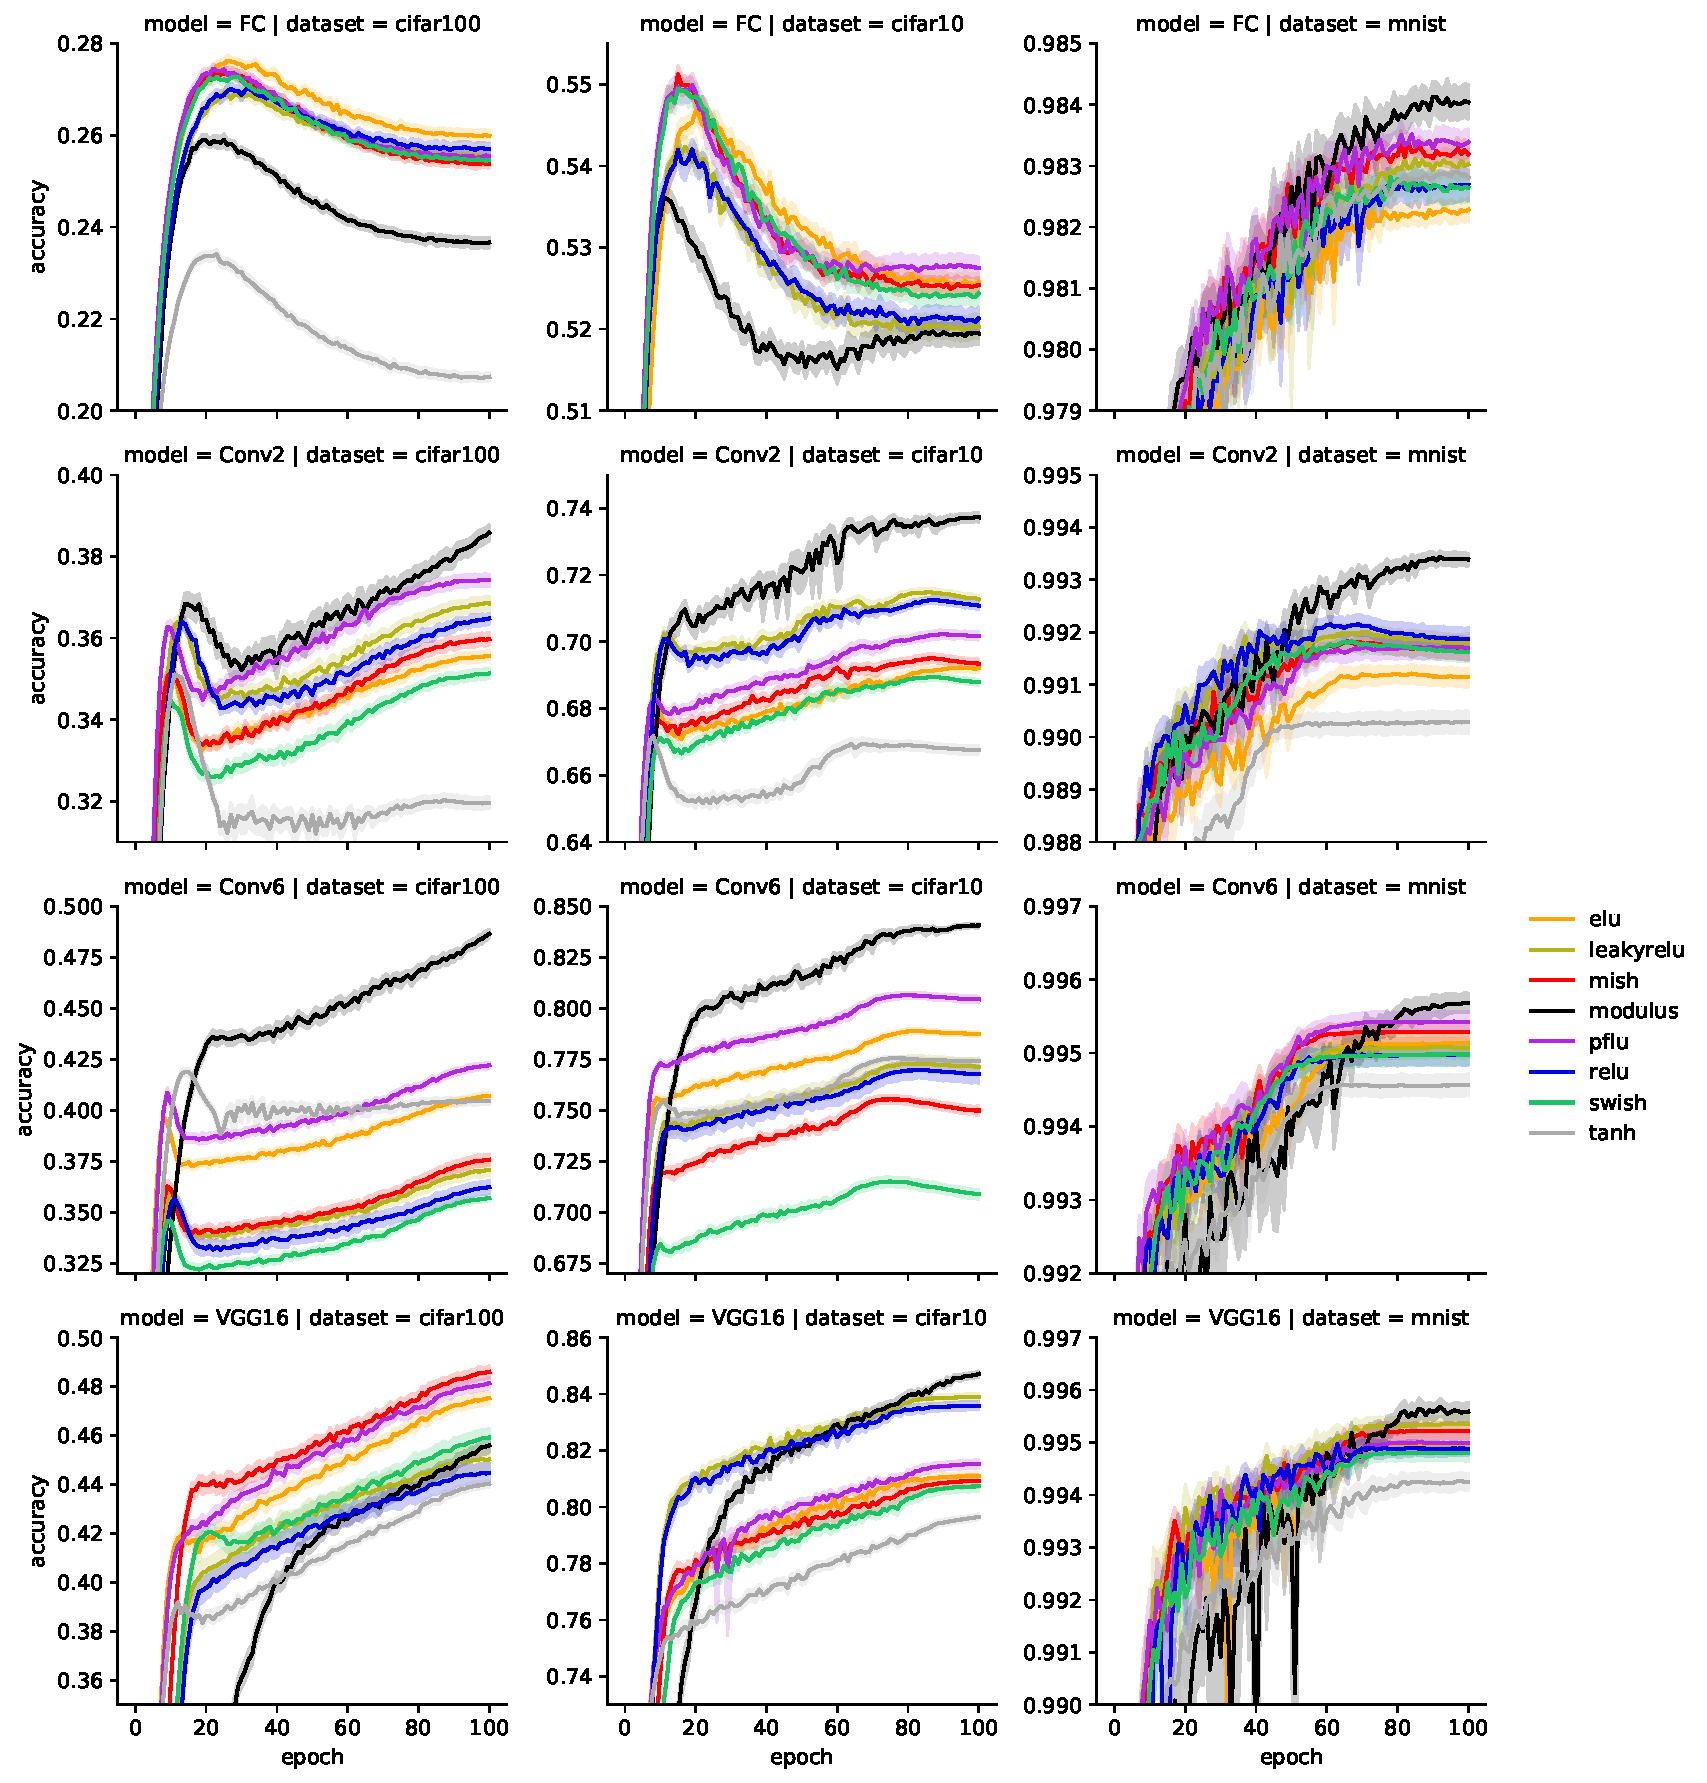
\includegraphics[width=1.0\linewidth]{modulus/images/training_curves}
	\caption{Training curves of all the trained models. Each line represents the average accuracy of 30 runs of a model. The shade beahind to each line shows the 95\% confidence interval around the mean. Notice that the scales in the y-axis are not shared to allow for better zoom in each figure, comparing the performance across models is not the objective of this study. Details like the shades are better viewed in a screen.}
	\label{fig:training_curves}
\end{figure}


The same experimental setup has been used across models, activations and datasets. All the networks have been trained for 100 epochs, and the best accuracy of each run has been recorded. Each run has been repeated 30 times with different random weight initializations. No \textit{dropout} \autocite{srivastava2014} nor \textit{batch normalization} \autocite{ioffe2015} have been used. \textit{Adam} \autocite{kingma14} has been used as optimizer, with a learning rate of $10^{-4}$, a \textit{gradual warmup} \autocite{gotmare2018} during the first 5 epochs starting from $10^{-5}$, and a \textit{cosine annealing} \autocite{loshchilov2017} with a target learning rate of $10^{-6}$ in the last epoch. The software versions used in all the chapter were: \textit{Python} 3.7.3, \textit{Pytorch} 1.7.1 and  \textit{TorchVision} 0.8.2. The code used in the experiments of this chapter can be found in the url included in the footnote \footnote{\url{https://github.com/ivallesp/abs}}.


\subsection{Results}
Table \ref{tab:modulus_results} summarizes the results of the classifiers for \textit{CIFAR10}, \textit{CIFAR100} and \textit{MNIST} datasets. As it can be seen from the tables, the \textit{modulus} activation function outperforms significantly the benchmark activations in 9 out of 12 experiments (4 architectures x 3 datasets). In 4 of these cases, the accuracy improvement is $3\%$ or higher, in relative terms. The \textit{SoftModulusT} approximation significantly outperforms the benchmark in 10 out of 12 experiments.

Figure \ref{fig:training_curves} shows the average training curves for the 12 experiments (the curves of the smooth approximations have been included in figure \ref{fig:training_curves_smooth} to compare them with the \textit{modulus}). As it can be noticed in several cases (e.g. \textit{CIFAR10-Conv2}, \textit{CIFAR10-Conv6}, \textit{CIFAR100-Conv6}), the accuracy of the networks with \textit{modulus} activation function keeps increasing at the 100th epoch while the benchmarks have already stabilized. That observation suggests that, if trained for longer, probably the accuracy would increase even more.


\begin{table}[hp!] \footnotesize  \setlength{\tabcolsep}{3pt}
	\caption{Accuracy comparison for the soft approximations of the \textit{modulus} function, compared with the original \textit{modulus} definition. The results are expressed as mean $\pm$ standard deviation across the 30 random initializations. The models with highest accuracy are highlighted in bold. A star is added to those cases where a \textit{SoftModulus} activation function achieved significantly higher results than the \textit{modulus}, with a significance level of $\alpha=0.05$.}
	\centering
	\begin{tabular}{rrcccc}
		\toprule
		 Dataset &   Activation &            FC             &           Conv2           &           Conv6           &           VGG16           \\ \midrule
		 CIFAR10 &      Modulus &     $53.97 \pm 0.24$      &     $73.93 \pm 0.42$      &     $84.22 \pm 0.29$      &     $84.86 \pm 0.32$      \\
		         & SoftModulusQ & $\mathbf{54.07 \pm 0.29}*$ &     $71.49 \pm 0.37$      &     $81.01 \pm 1.27$      &     $10.00 \pm 0.00$      \\
		         & SoftModulusT &     $54.04 \pm 0.24$      & $\mathbf{73.95 \pm 0.40}$ & $\mathbf{84.36 \pm 0.28}$ & $\mathbf{85.34 \pm 0.36}*$ \\ \midrule

		CIFAR100 &      Modulus &     $26.29 \pm 0.26$      &     $38.66 \pm 0.56$      & $\mathbf{48.73 \pm 0.62}$ &     $45.83 \pm 0.80$      \\
		         & SoftModulusQ &     $26.23 \pm 0.25$      &     $37.48 \pm 0.44$      &     $48.16 \pm 1.97$      &      $1.00 \pm 0.00$      \\
		         & SoftModulusT & $\mathbf{26.32 \pm 0.24}$ & $\mathbf{38.69 \pm 0.56}$ &     $48.63 \pm 0.83$      & $\mathbf{48.47 \pm 0.68}*$ \\ \midrule

		   MNIST &      Modulus &     $98.47 \pm 0.07$      &     $99.38 \pm 0.04$      &     $99.60 \pm 0.03$      & $\mathbf{99.63 \pm 0.04}$ \\
		         & SoftModulusQ & $\mathbf{98.51 \pm 0.06}*$ &     $99.37 \pm 0.03$      & $\mathbf{99.62 \pm 0.03}*$ &     $11.35 \pm 0.00$      \\
		         & SoftModulusT &     $98.47 \pm 0.06$      & $\mathbf{99.39 \pm 0.04}$ &     $99.61 \pm 0.03$      &     $99.62 \pm 0.03$      \\ \bottomrule
	\end{tabular}
	\label{tab:modulus_results_smooth}
\end{table}

\begin{figure}[h!]
	\centering
	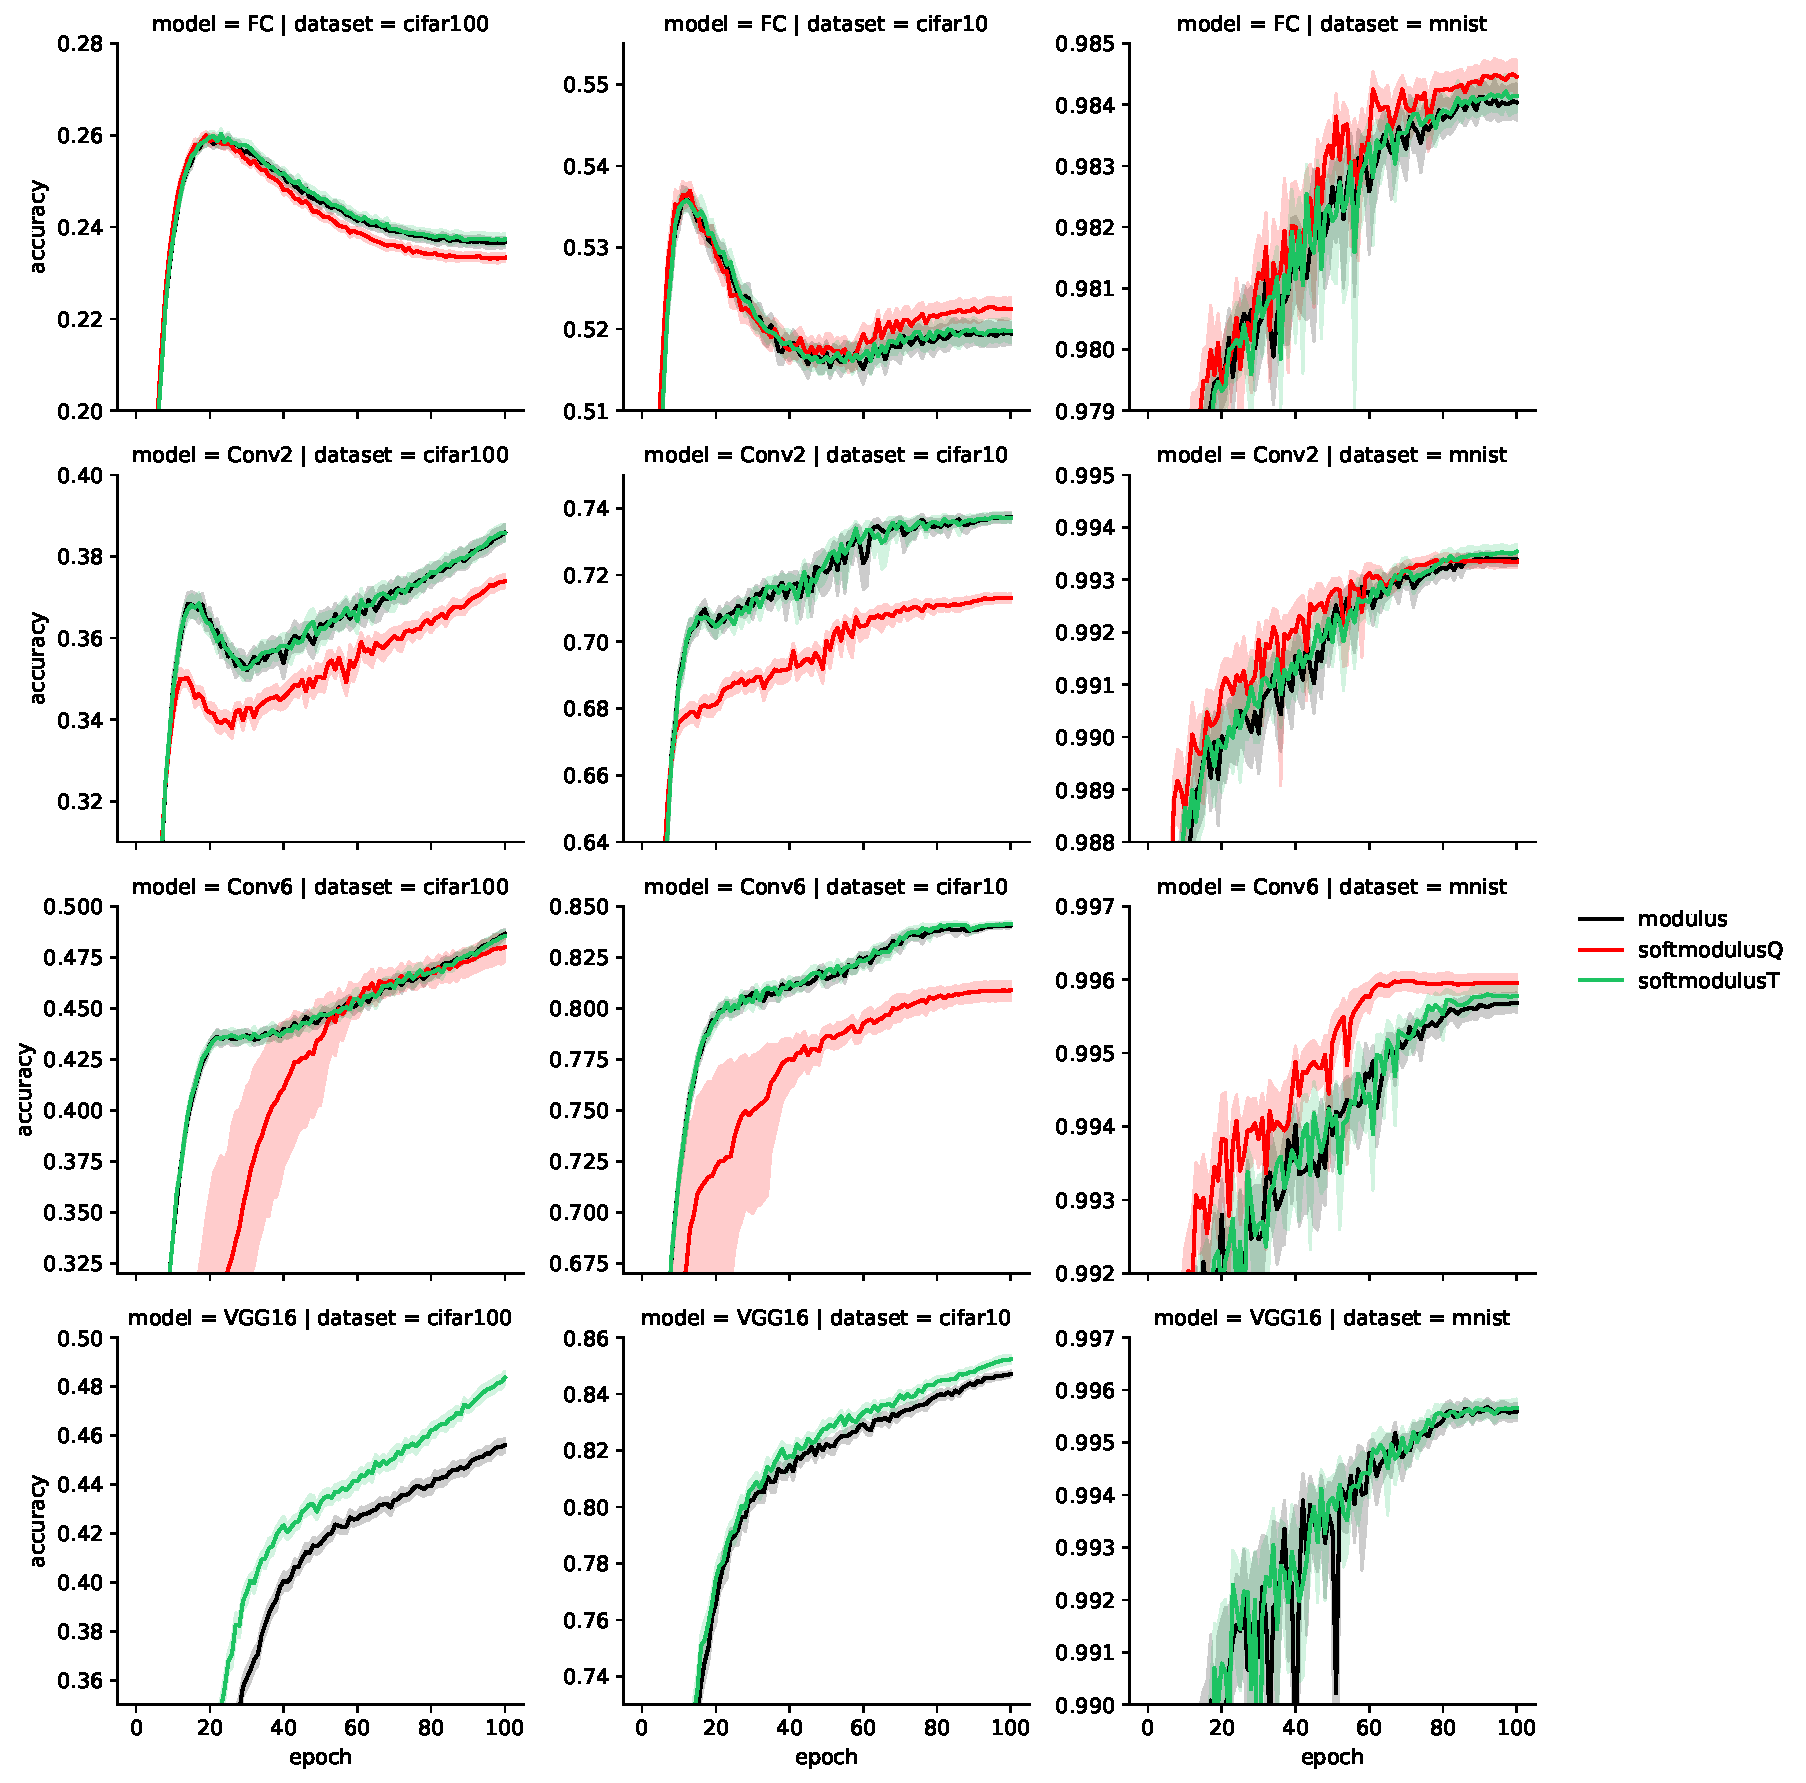
\includegraphics[width=1.0\linewidth]{modulus/images/training_curves_smooth}
	\caption{Training curves smooth approximations compared with the \textit{modulus}. Each line represents the average accuracy of 30 runs of a model. The shade behind to each line shows the 95\% confidence interval around the mean. Notice that the scales in the y-axis are not shared to allow for better zoom in each figure, comparing the performance across models is not the objective of this study. Details like the shades are better viewed in a screen.}
	\label{fig:training_curves_smooth}
\end{figure}

The results of the \textit{SoftModulus} approximations compared with the \textit{modulus} activation function are summarized in table \ref{tab:modulus_results_smooth}. Additionally, figure \ref{fig:training_curves_smooth} shows the training curves for the same activations. The \textit{SoftModulusQ} approximation achieved significantly better results than the original modulus in several cases (\textit{FC} model over \textit{CIFAR10} and \textit{MNIST} dataset, and \textit{Conv6} over \textit{MNIST} dataset); however it seems to be much more unstable: on VGG16, the gradients of the models with \textit{SoftModulusQ} activations vanish at the beginning of the training process due to the fact that the weights are initialized very close to zero and the gradients are too small, causing numerical issues. This problem may be solved tweaking the initialiation. However, the \textit{SoftModulusT} approximation seems to be on-par with the original \textit{modulus} in the majority of cases, while it performs significantly better for deep architectures like \textit{VGG16}. A plausible hypotyhesis explaining that observation is  that the difference between the two approximations is due to the width of the zero gradient region around $x=0$: wider regions lead to more training problems (see figure \ref{fig:activationssmooth}). The $\beta$ parameter in the hyperbolic tangent approximation allows for easily adjust this zero-gradient region. Different values of beta were informally tested concluding that for high values of $\beta$ (e.g. $\beta=1.0$) the model struggles to train due to numerical precision problems (small values of weights lead to tiny gradients). A value of $\beta=0.01$ seems to work well for all the tested experiments. Finally, the \textit{SoftModulusT} approximation achieves superior results than the original \textit{modulus} when used in the \textit{VGG16} architecture.




\section{Conclusions} \label{sec:modulus_conclusions}
This chapter provides evidences of how the proposed \textit{modulus} activation function outperforms the benchmark activation functions in 75\% of the experiments. The improvement achieved by the networks with this activation function is often significantly higher ($3\%$ or higher in 33.3$\%$ of the experiments conducted). Additionally, a smooth version of the \textit{modulus} activation function is proposed, even performs better than the first one, at a slightly higher computational cost.

The results of this chapter motivate exploring non-monotonic activation functions as alternatives to the classical choices.





%!TEX root = ../thesis.tex
\chapter{Distilling the knowledge of pretrained models} \label{ch:distillation}
\section{Overview}
Since the 2012 \textit{ImageNet} competition, many convolutional neural networks based architectures for computer vision have been proposed leading to a large number of open source resources in the form of pre-trained models. In this chapter we explore the idea of combining the knowledge of multiple pre-trained models into another simpler pre-trained model using knowledge distillation techniques. We show how we can improve the accuracy of the lightest pre-trained models by fine-tuning them using the soft-labels of their superior counterparts. The knowledge transfer is performed by using solely unlabeled data. We achieved up to a 3.0\% and a 1.7\% absolute improvement in top-1 and top-5 accuracy is achieved across several models, suggesting that the trained architectures are still not at their capacity limit. This technique allows having a significant improvement of performance in mobile and other \textit{TinyML} applications \autocite{sanchez2020}.

 All the code used in this chapter is publicly available in a repository\footnote{\url{https://github.com/ivallesp/distillnet}}.

\section{Introduction}
Computer vision systems have evolved dramatically in the last decade due to the rise of deep learning technologies. In 2012, \textit{AlexNet} \autocite{krizhevsky2012} achieved the first position in the \textit{ImageNet} yearly challenge \autocite{ILSVRC15}, and that was the first time a neural network got such position. Since then, the neural solutions have prevailed, and many different architectures have been proposed, each of them being better than the previous ones \autocite{khan2020, algan2021}. The weights of many of the best solutions to the \textit{ImageNet} competition are publicly available (e.g. \autocite{he2016, chollet2017, szegedy2016, szegedy2017, howard2017, pham2018, tan2019}), and the machine learning community gets benefits from it. One of the most common applications of pre-trained models is transfer learning \autocite{huang2021} (as briefly discussed in section \ref{sec:typesoflearning_others}), where the weights of a model that has previously been trained to solve a large scale pretext task (such as the \textit{ImageNet} classification task) are re-utilized and fine-tuned to adapt them to another task. Usually, the first layers of the network are frozen and only the last few layers are allowed to be adjusted. This simple idea has been developed in the last years, and many further studies have been published (see \autocite{zhu2018, wu2021, pzhao2021}). Transfer learning works under the hypothesis that lower layers learn simpler and widely applicable patterns that are used by higher level layers to solve the objective task.

Another very powerful technique is known as knowledge distillation, and consists of transferring knowledge from a teacher model to a student model. In 2015, \textit{Geoffrey Hinton} and his collaborators showed that it was possible to improve the performance of a simple model (known as the student) by distilling the knowledge of a more sophisticated model (named the teacher) \autocite{hinton2015}. The technique proposed in this chapter is very simple and consists of training the student with the soft-targets of the teacher, given a transfer data set. The soft-targets are the raw predictions of the model, which are expressed as probabilities of belonging to each class. The authors suggest to minimize the cross-entropy with soft-targets, after dividing the logits by a temperature constant $\mathcal{T}$ (process known as warming the logits, extra details in section \ref{sec:distillation_kd}) so that the probability distribution gets less sparse (i.e. more spread across the classes different than the majority class). This technique is built over the hypothesis that there is more information in the soft targets than in the hard targets. This additional information is sometimes known as \textit{dark knowledge} \autocite{gou2020}. Knowledge distillation is still a hot topic in nowadays research (see \autocite{tan2021, zhao2021, lee2021}).


This work explores the idea of combining the knowledge of multiple pre-trained models with the objective of reducing the large computation required for running top-tier computer vision models, through improving the accuracy of a base low-resource model, while keeping the training cost small and using an unlabeled transfer data set. 	An ensemble of pre-trained models may be the most powerful solution in terms of accuracy but it is energy-inefficient and may not be applicable for mobile applications, tasks that require a time-sensitive inference \autocite{sanchez2020} or other \textit{TinyML} tasks. Therefore, we approach this problem from a knowledge distillation perspective, where we aim to distill the knowledge of multiple heavy pre-trained models into a light-weight base model. We show that not only it is possible to improve its original accuracy but that some techniques for combining the knowledge of multiple teachers are better than others.

We find many scenarios that can be benefited from the results of this study. The first one is data intense applications such as video event detection \autocite{chakraborty2021} (for instance in autonomous driving \autocite{swaminathan2019}), where a large number of frames need to be processed in real time and with a high performance. The second one is the tasks that need to run necessarily in a low-resource device, like mobile devices (e.g. augmented reality for map localization \autocite{limmer2017}), or the time-sensitive tasks (e.g. facial recognition for security \autocite{aung2021}). Finally, the proposed models are more environmental-friendly, as they require less energy for training and inference \autocite{wu2022sustainable}.

A few previous works have been published where the objective was to combine multiple deep learning models. The authors of \autocite{liu2020b} distill the knowledge of several teachers into a multitask student in the computational linguistics domain. Apart from the different domain of application, their approach differs from ours in the fact that their student and teachers goals differ: their student learns to combine the different objectives of the teachers. In \autocite{geyer2019}, the authors present a new technique that allows merging multiple models using a parameter fusing technique based on the Incremental Mode Matching (IMM) procedure \autocite{lee2017}. This methodology has an important limitation that makes it unsuitable for our use case: the pre-trained and the target architecture must have the same structure. Our objective is to improve the performance of a light-weight model using the knowledge of its greater siblings, which normally have more complex architectures. In the work of \autocite{asif2019}, the authors define a framework to learn a small ensemble of students from a large ensemble of teachers which are combined linearly. For that, they propose to define a neural network architecture with as many student branches as teachers. The student branches are trained to minimize their \textit{Kullback-Leibler} (KL) divergence with their corresponding teacher branch, as well as minimizing the KL-divergence between the linear combination of the students, and the linear combination of the teachers. Our approach differs fundamentally in the fact that our base architecture size is independent of the number of teachers. In addition, instead of using KL-divergence losses, we minimize the cross-entropy with soft-targets, as defined by \autocite{hinton2015}.

In this work we show how the performance of small pre-trained models can be increased by leveraging the knowledge of their large counterparts. The knowledge distillation, pre-trained models and teacher combination methods are described in section  \ref{sec:distillation_methods}. Section \ref{sec:distillation_experiments} provides the details of our experimental framework, including the data set used along this study as well as the different experiments conducted. The results of the experiments are presented and analyzed in section \ref{sec:distillation_results}. Finally, the section \ref{sec:distillation_conclusions} summarizes the conclusions drawn from the achieved results.

\section{Methods} \label{sec:distillation_methods}
In this section we describe the training methods we used as well as the knowledge distillation framework and the techniques employed to combine different teachers.

\subsection{Knowledge distillation} \label{sec:distillation_kd}
The original knowledge distillation method, as defined by \autocite{hinton2015}, consists of using the $||C||$ class probabilities (known as soft-targets) produced by a machine learning model (named the teacher) as the training objective for another, often simpler, machine learning model (named the student). The probabilities of a deep learning model $\mathbf{p_i}$ (where $i \in \{1,...,||C||\}$) are normally calculated by applying the softmax function over its logits $\mathbf{z}$ \autocite{Goodfellow2016}. Usually, a temperature parameter $\mathcal{T}$ is introduced with the aim of producing a softer probability distribution over the classes (see equation \ref{eq:softmax}, where $i$ and $j$ represent class indices).

\begin{equation}
p_{i \in \{1 .. C\}} = \frac{\exp(z_{ti}/\mathcal{T})}{\sum_j^C \exp(z_{tj}/\mathcal{T})}
\label{eq:softmax}
\end{equation}

The authors of \autocite{hinton2015} also recommend combining two targets: cross-entropy with soft-targets $J_S$ and cross-entropy with hard-targets  $J_H$. The first objective is computed with an increased temperature, while the second one is computed with $\mathcal{T}=1$. See the losses definitions in equations \ref{eq:ced} and \ref{eq:ces}, where $\mathbf{z_t}$ and $\mathbf{z_s}$ denote the logits for the teacher and the student, respectively, and $\mathbf{y}$ denotes the ground truth label. The losses are combined as shown in equation \ref{eq:loss_distillation}, where the $\alpha$ parameter is intended to balance between the two losses \autocite{gou2020}.

\begin{equation}
J_S\left[p( \mathbf{z_t}, \mathcal{T}), p(\mathbf{z_s},\mathcal{T}) \right] = -\sum_i p_i(z_{ti}, \mathcal{T}) \log \left(p_i(z_{si, \mathcal{T}})\right)
\label{eq:ced}
\end{equation}

\begin{equation}
J_{H}\left[\mathbf{y}, p(\mathbf{z_s}, \mathcal{T}=1) \right] = -\sum_i y_i \log \left(p_i(z_{si})\right)
\label{eq:ces}
\end{equation}

\begin{equation}
J = \alpha J_S + (1-\alpha) J_{H}
\label{eq:loss_distillation}
\end{equation}

In this study we fix $\alpha=1$ given that we only use unlabeled data for training, and hence no hard targets are available.

\subsection{Teachers combination} \label{sec:distillation_teachers_comb}
Different models may produce harder or softer posterior probability distributions. In order to be able to successfully combine  different models for building the teacher signal that will be used to train the student, the posterior probability distributions need to be calibrated.

The hardness or softness of a distribution can be controlled with the temperature parameter $\mathcal{T}$ (see equation \ref{eq:softmax}). In this case, as different models have been combined to build the soft target signal. The temperature of each model has been chosen so that the average probability of the most probable class becomes $P_1$. Hence $P_1$ represents a hyperparameter that must be chosen before training. We use $p_1$ to denote a specific choice of $P_1$.  $\mathcal{T}$ has been determined independently for each pre-trained model so that $P_1=p_1$, on average over the transfer data set. The value of $\mathcal{T}$ has been found using the bisection method (using $\mathcal{T}=1$ as initial value).

Once the probability distributions have been normalized, the following techniques have been defined as teacher combination proposals.

\begin{itemize}
 	\item Mean: arithmetic mean across the set of $R$ teachers, for every instance $x$ and class $c$.
 	$$p_{\text{mean}}(c|x) = \frac{1}{R} \sum_{r=1}^R p_{r}(c|x)$$
 	\item Median: median across the set of $N$ teachers, for every instance $x$ and class $c$. The result of this operation needs to be normalized so that the probabilities across the $C$ different classes sum to 1. $$p_{\text{median}}(c|x) = \frac{1}{M} \ \text{median}_r( p_{r}(c|x)) \quad \text{where} \quad M = \sum_{c=1}^C  \text{median}_r( p_{r}(c|x))$$
 	\item Random: the probabilities of each instance $x$ are selected from a random teacher $\hat{r}$. The randomization is reset after every training epoch.
 	$$\hat{r} \sim U(1, \mathcal{R}) \rightarrow \mathbf{p_\text{random}}(x) = \mathbf{p_{\hat{r}}}(x)$$
	\end{itemize}

\subsection{Pretrained models}
Some of the pre-trained models included in the \textit{Keras} library for \textit{Python} \autocite{chollet2015keras} have been used along this study. Below we provide a short description about each of those architectures, and further details are included in table \ref{table:models}.

\begin{enumerate}
   	\item \textit{ResNet} \autocite{he2016}: convolutional neural network with multiple blocks where the output of the $l^{th}$ layer is added to the output of the $(l+1)^{th}$. This structure is known as \textit{residual connection} (or \textit{skip connection}), and leads to the following transition: $x_{l+1} = f_{l+1}(x_{l}) + x_l$, where $f$ represents a convolutional layer. Described in the section \ref{sec:deepernn}.
   	\item \textit{Inception ResNet} \autocite{szegedy2017}: introduction of the \textit{residual connection} structure from \autocite{he2016} to the classical \textit{inception} convolutional neural network model, combined with several efficiency tricks. The \textit{inception} model is based on the idea of using different convolution operations (with different receptive field sizes and pooling operations) in every layer, and concatenating the result together. Additionally, before each regular 2D convolution, a 1x1 convolutional layer is introduced to optimize the computation.
   	\item \textit{DenseNet} \autocite{huang2017}: convolutional neural network inspired by the \textit{ResNet} model \autocite{he2016} that introduces direct connections from every layer to all the subsequent ones leading to the following transition: $x_{l+1} = f_l([x_0, x_1, ... x_{l-1}])$. The square brackets in the previous expression mean concatenation.
   	\item \textit{NASNet} \autocite{pham2018}: convolutional neural network designed using Neural Architecture Search (NAS) with reinforcement learning algorithms. The final architecture structure resembles to \textit{inception} \textit{ResNet}, but has been optimized to have a higher inductive bias.
   	\item \textit{Xception} \autocite{chollet2017}: convolutional architecture inspired in \textit{InceptionV3}  \autocite{szegedy2016} that features \textit{depthwise separable convolutions} for higher computational efficiency.
   	\item \textit{MobileNet V1} and \textit{V2} \autocite{howard2017, sandler2018}: convolutional architecture designed to be efficient and scalable with the objective of being implemented into mobile devices. These networks feature \textit{depthwise-separable convolutions} for reducing the number of parameters, compression-expansion blocks and the introduction of two parameters $\alpha$ and $\rho$ to control the depth of the network and the input image resolution, respectively.
   	\item \textit{EfficientNet} \autocite{tan2019}: highly scalable convolutional architecture that attempts to tie the network depth, width and the input image resolution  together into a compound single parameter referred as $\phi$. The architecture of the base model (aka \textit{EfficientNet}) has been designed using NAS techniques.
\end{enumerate}


\begin{table}[h]
	\small
	\caption{Pretrained models used as teachers along this study, taken from \textit{Keras} implementations. Some of the input resolutions shown in the table may not correspond to the resolutions of the original papers, however we decided to run the models in the resolutions indicated in the table as they showed a substantial performance improvement. The performance metrics reported in the table are empirical accuracies obtained by measuring the performance of the models against the \textit{ImageNet} 2012 validation dataset, using the \textit{Keras} implementations. They may differ from the performance reported in the original studies. $m$ means millions. We have marked in bold the models that were used as students.}
	\centering
\begin{tabular}{c|cc|cc}
	\toprule
	         Model          & Input size & \#Params. & Top-1 acc. & Top-5 acc. \\ \midrule
	      NasNetLarge       &  331x331   &    89m    &  82.44\%   &  96.02\%   \\
	   InceptionResNetV2    &  299x299   &    56m    &  80.44\%   &  95.31\%   \\
	   \textbf{Xception}    &  299x299   &    23m   &  78.92\%   &  94.47\%   \\
	    EfficientNetB7      &  256x256   &    67m   &  77.88\%   &  93.87\%   \\
	      DenseNet201       &  256x256   &    20m    &  77.75\%   &  93.83\%   \\
	      DenseNet169       &  256x256   &    14m    &  76.60\%   &  93.39\%   \\
	       ResNet50         &  256x256   &    26m   &  75.53\%   &  92.53\%   \\
	 \textbf{DenseNet121}   &  256x256   &    8m     &  75.47\%   &  92.68\%   \\
	\textbf{EfficientNetB0} &  256x256   &    5m     &  75.17\%   &  92.34\%   \\
	 \textbf{MobileNetV2}   &  256x256   &    4m     &  73.11\%   &  91.29\%   \\
	      MobileNetV1       &  256x256   &    4m    &  71.73\%   &  90.44\%   \\ \bottomrule
\end{tabular}
\label{table:models}
\end{table}

\section{Experiments} \label{sec:distillation_experiments}
In this section we first provide an overview of the data set that has been used to conduct the study, describe the experiments performed and show our results.

\subsection{Data set}
The \textit{ILSVRC2012 ImageNet} data set has been used in all our experiments \autocite{ILSVRC15}, given its large popularity and numerous available benchmarks. It is composed of 1.3 million images,  each of which belongs to only one class out of 1000 available classes. The data is provided in three separated subsets: train, validation and test, with 1.2M, 50,000 and 100,000 images in each set, respectively. The ground truth labels are provided for the train and validation sets, but not for the test set (i.e. the test set is unlabeled).

The original data set comes with images at different sizes and aspect ratios. We have generated three different sets with the following sizes: 256x256, 299x299 and 331x331. For that, we have first resized the images so that their short edge matches the desired size and then we have applied center-cropping to get a square image, as it is common in these cases. Pixel values centering and scaling have been applied as per the functions provided with \textit{Keras} along with each pre-trained model. No data augmentation has been used along this study.

In this work, we will use the unlabeled test set as transfer data set and the validation set to measure and report performance.

\subsection{Experimental framework}
We have done several experiments to prove that the methodology described in this study scales to different settings. In those experiments, we varied the following factors:

\begin{itemize}
	\item Student: we used different small models as a base, to study how the methodology works with different students. The models used as students are: \textit{MobileNetV2}, \textit{EfficientNetB0}, \textit{DenseNet121} and \textit{Xception}.
	\item Teachers set: according to the performance shown in table \ref{table:models}, we selected different sets of teachers to combine to build the distillation target: the ``best'' teacher (i.e. \textit{NasNetLarge}), the ``top-3'' teachers (i.e. \textit{NasNetLarge}, \textit{InceptionResNetV2} and \textit{Xception}) and ``all'' the 11 teachers.
	\item Teachers combination method: we tried to combine the teachers with the methods described in the section \ref{sec:distillation_teachers_comb}. These methods are referred in the tables below as ``mean'', ``median'' and ``random''. This does not apply to the case where we only consider the best teacher, as no combination method is needed
\end{itemize}

The set of experiments conducted in this study is represented in the schema of figure \ref{fig:schema}.

% TODO: \usepackage{graphicx} required
\begin{figure}[h!]
\centering
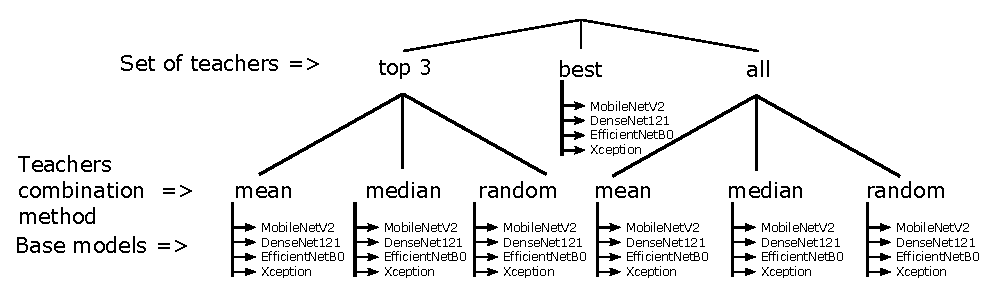
\includegraphics[width=0.9\linewidth]{distillation/images/schema}
\caption{Schema representing the set of experiments conducted in this study.}
\label{fig:schema}
\end{figure}


We have repeated each experiment 5 times to add more robustness to our results, totaling to 140 training processes. The students initial weights have always been fixed to the pre-trained weights for the \textit{ImageNet} classification task, across all the experiments. During training, no layers have been frozen, allowing the optimizer to fine-tune all the weights in the student network. The temperature of the softmax in the output of the last layer has been increased in all the cases to match the normalized soft-targets distribution, as described in section \ref{sec:distillation_teachers_comb}.  Each model has been trained for 100 epochs, and the results are presented in the next section at the early stopping point. We used \textit{Adam} optimizer \autocite{kingma14} and a learning rate of $\lambda = 10^{-6}$.

In our experiments we fix\footnote{The $P_1$ value has been chosen to be close to the minimum average probability across teachers of the most probable class.} $P_1=0.35$ and determine the value of $\mathcal{T}$ for every pre-trained model using the bisection method with the transfer data set. The value of $P_1$ has been chosen so that it produces an average temperature across the models of 2.0, which is close to the range recommended in \autocite{hinton2015}. We tried doubling the temperature parameter concluding that there were no noticeable improvements.

To run the experiments, we used a single \textit{Nvidia RTX 2080ti} GPU, and the code has been implemented in \textit{Tensorflow 2.0}. The repository of code is public and can be found in URL of the footnote\footnote{\url{https://github.com/ivallesp/distillnet}}.

\subsection{Results}  \label{sec:distillation_results}
Tables \ref{tab:distillation_results1} and \ref{tab:distillation_results5} summarize the results achieved by each of the experiments run over the \textit{ImageNet} data set. The metrics reported are the top-1 accuracy and the top-5 accuracy, as it is standard in \textit{Imagenet} benchmarks, at the early stopping epoch. The results are expressed as the average metric $\pm$ the standard error\footnote{It is important to clarify that the standard error of the results shown in the tables is very small because the initial weights in each student are the same across the 5 repetitions, given that the training starts from the pre-trained model weights. The variability reported is produced by stochastic processes other than the initialization, such as dropout or random teacher selection.}.

As it can be seen in the table, the proposed methodology achieves an absolute accuracy increase of up to +3.04\%, +1.00\%, +0.97\% and +0.38\% for the \textit{EfficientNetB0}, \textit{MobileNetV2},  \textit{DenseNet} and \textit{Xception} students, respectively.

We observe that building a teacher by combining ``all'' the pre-trained models, or combining the ``top-3'' ones, leads to similar results. However, in some cases the combination of ``all' the teachers is superior to the ``top-3'' (e.g. \textit{DenseNet121} as student), but also the contrary occurs (e.g. \textit{EfficientNetB0} as student). We also notice that using only the ``best'' model as teacher often leads to overfitting issues.

Regarding the teacher combination method, we observe that the ``mean'' and ``random'' methods lead to better results when compared to the ``median'' method. This may be happening because, when using the ``median'' method to combine the teacher predictions, the probability distribution is not preserved (i.e. the output probabilities for every class do not sum to 1), forcing us to apply a posterior normalization step. This process may add some noise to the new distillation target.

The aforementioned observations lead to the following conclusions: (1) the smaller the student model is, the higher the accuracy increase, (2) increasing the number of teachers leads to better generalization, and (3) combining the teachers using an average or a random teacher choice results in better performance than combining them using the median.

\begin{table}[h]
\footnotesize
\centering

\caption{Results in top-1 accuracy (\%) for all the experiments. Each column in the table represents a different teacher set. We highlighted in bold the experiment that achieved better performance for each student.}
\begin{tabular}{rrrrrr}
	\toprule
             &              & Baseline &              Best &              Top3 &               All \\
    Student, & Comb. method &          &                   &                   &                   \\ \midrule
 MobileNetV2 &         Mean &    73.11& $ 73.85 \pm 0.01$ &  $73.99 \pm 0.01$ &  $\mathbf{74.11 \pm 0.02}$ \\
             &       Median &    73.11 &                 - &  $75.92 \pm 0.00$ &  $74.04 \pm 0.01$ \\
             &       Random &    73.11 &                 - &  $73.96 \pm 0.01$ &  $74.03 \pm 0.01$ \\
             &              &          &                   &                   &                   \\
	EfficientNetB0 &         Mean &    75.17 & $ 78.14 \pm 0.02$ &  $78.20 \pm 0.02$ &  $78.07 \pm 0.01$ \\
             &       Median &    75.17 &                 - &  $78.18 \pm 0.01$ &  $77.98 \pm 0.01$ \\
             &       Random &    75.17 &                 - &  $\mathbf{78.21 \pm 0.01}$ &  $78.05 \pm 0.01$ \\
             &              &          &                   &                   &                   \\
 DenseNet121 &         Mean &    75.47 & $ 75.83 \pm 0.01$ &  $75.92 \pm 0.01$ &  $\mathbf{76.44 \pm 0.02}$ \\
             &       Median &    75.47 &                 - & $ 75.87 \pm 0.02$ & $ 76.42 \pm 0.02$ \\
             &       Random &    75.47 &                 - &  $75.92 \pm 0.02$ &  $76.43 \pm 0.01$ \\
             &              &          &                   &                   &                   \\
    Xception &         Mean &    78.92 &  $79.11 \pm 0.01$ &  $\mathbf{79.30 \pm 0.02}$ &  $79.16 \pm 0.02$ \\
             &       Median &    78.92 &                 - &  $79.18 \pm 0.01$ &  $79.19 \pm 0.01$ \\
             &       Random &    78.92 &                 - &  $79.27 \pm 0.02$ &   $79.14\pm 0.01$ \\ \bottomrule
\end{tabular}
\label{tab:distillation_results1}
\end{table}

\begin{table}[h]
\footnotesize
\centering

\caption{Results in top-5 accuracy (\%) for all the experiments. Each column in the table represents a different teacher set. We highlighted in bold the experiment that achieved better performance for each student.}
\begin{tabular}{rrrrrr}
	\toprule
             &              & Baseline &             Best &             Top3 &              All \\
    Student & Comb. method &          &                  &                  &                  \\ \midrule
 MobileNetV2 &         Mean &      91.29 & $91.83 \pm 0.01$ & $91.86 \pm 0.01$ & $92.02 \pm 0.01$ \\
             &       Median &      91.29 &                - & $91.84 \pm 0.01$ & $91.91 \pm 0.01$ \\
             &       Random &      91.29 &                - & $91.88 \pm 0.00$ & $\mathbf{91.96 \pm 0.01}$ \\
             &              &          &                  &                  &                  \\
	EfficientNetB0 &         Mean &      92.34 & $94.17 \pm 0.00 $ & $\mathbf{94.17 \pm 0.01}$ & $94.01 \pm 0.00$ \\
             &       Median &      92.34 &                - & $94.10 \pm 0.01$ & $93.93 \pm 0.01$ \\
             &       Random &      92.34 &                - & $94.08 \pm 0.01$ & $93.99 \pm 0.01$ \\
             &              &          &                  &                  &                  \\
 DenseNet121 &         Mean &      92.68 & $92.95 \pm 0.01 $ & $93.04 \pm 0.01$ & $\mathbf{93.30 \pm 0.01}$ \\
             &       Median &      92.68 &                - & $92.98 \pm 0.01$ & $93.29 \pm 0.01$ \\
             &       Random &      92.68 &                - & $93.03 \pm 0.01$ & $\mathbf{93.30 \pm 0.01}$ \\
             &              &          &                  &                  &                  \\
    Xception &         Mean &     94.47& $94.55 \pm 0.01$ & $\mathbf{94.70 \pm 0.01}$ & $94.65 \pm 0.00$ \\
             &       Median &      94.47 &                - & $94.65 \pm 0.01$ & $94.63 \pm 0.01$ \\
             &       Random &      94.47 &                - & $94.68 \pm 0.01$ & $94.59 \pm 0.01$ \\ \bottomrule
\end{tabular}
\label{tab:distillation_results5}
\end{table}

% TODO: \usepackage{graphicx} required
\begin{figure}[h!]
\centering
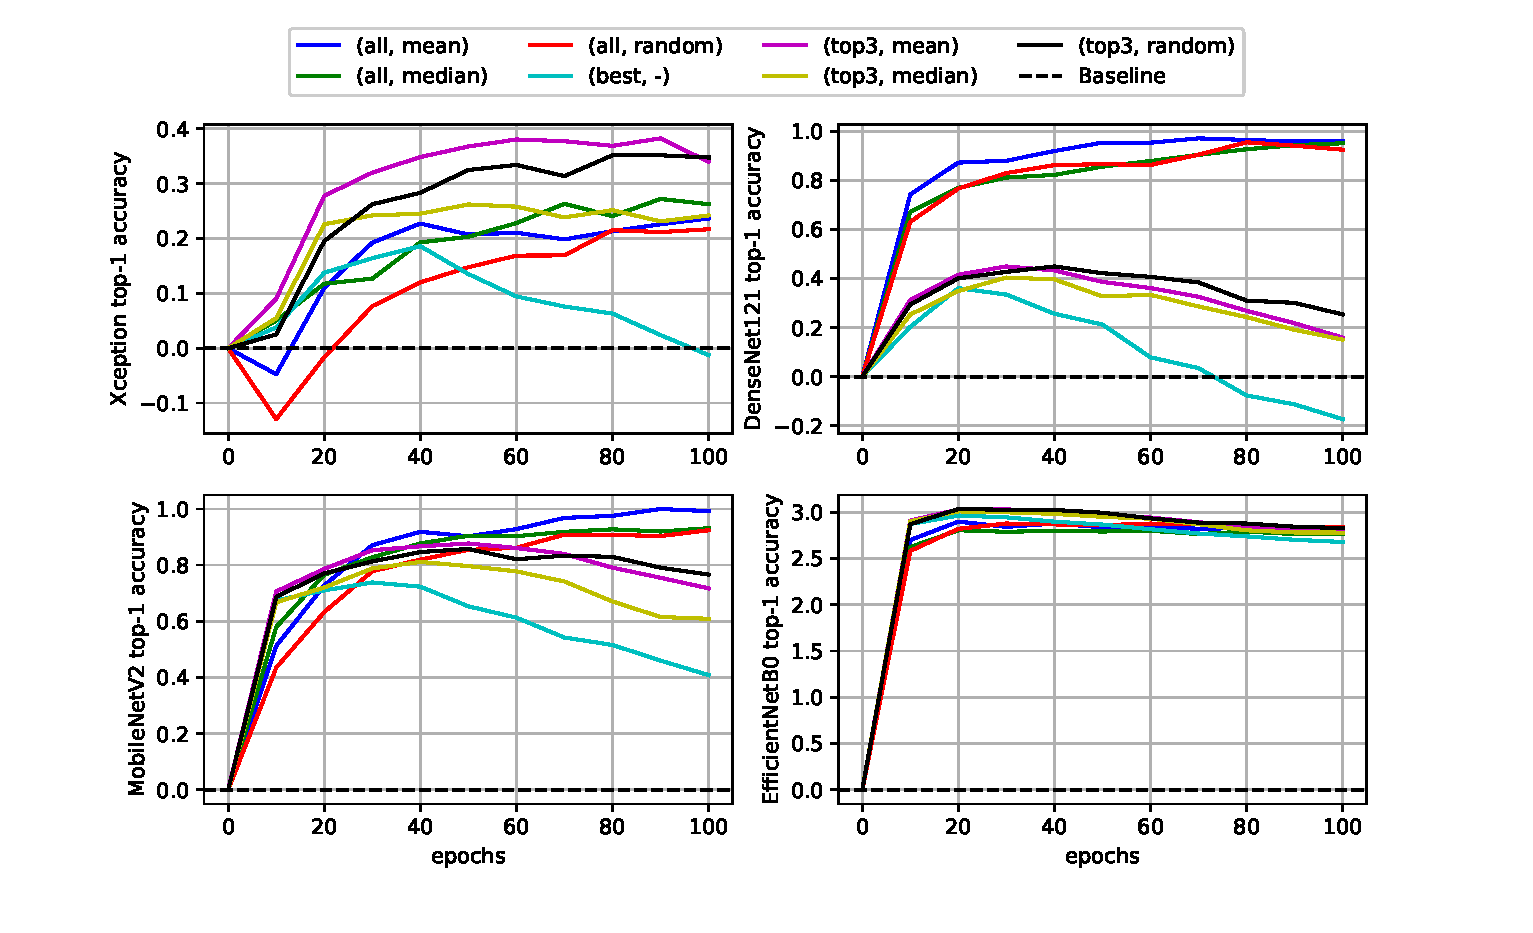
\includegraphics[width=1\linewidth]{distillation/images/top1_curves}
\caption{Absolute difference of top-1 accuracy with respect to the baseline. The x-axis represents the number of training epochs and the tuples in the legend are expressed in the following format: (teachers set, combination method). The y-axis shows the absolute difference in performance with respect to the baseline.}
\label{fig:top1curves}
\end{figure}


% TODO: \usepackage{graphicx} required
\begin{figure}[h!]
\centering
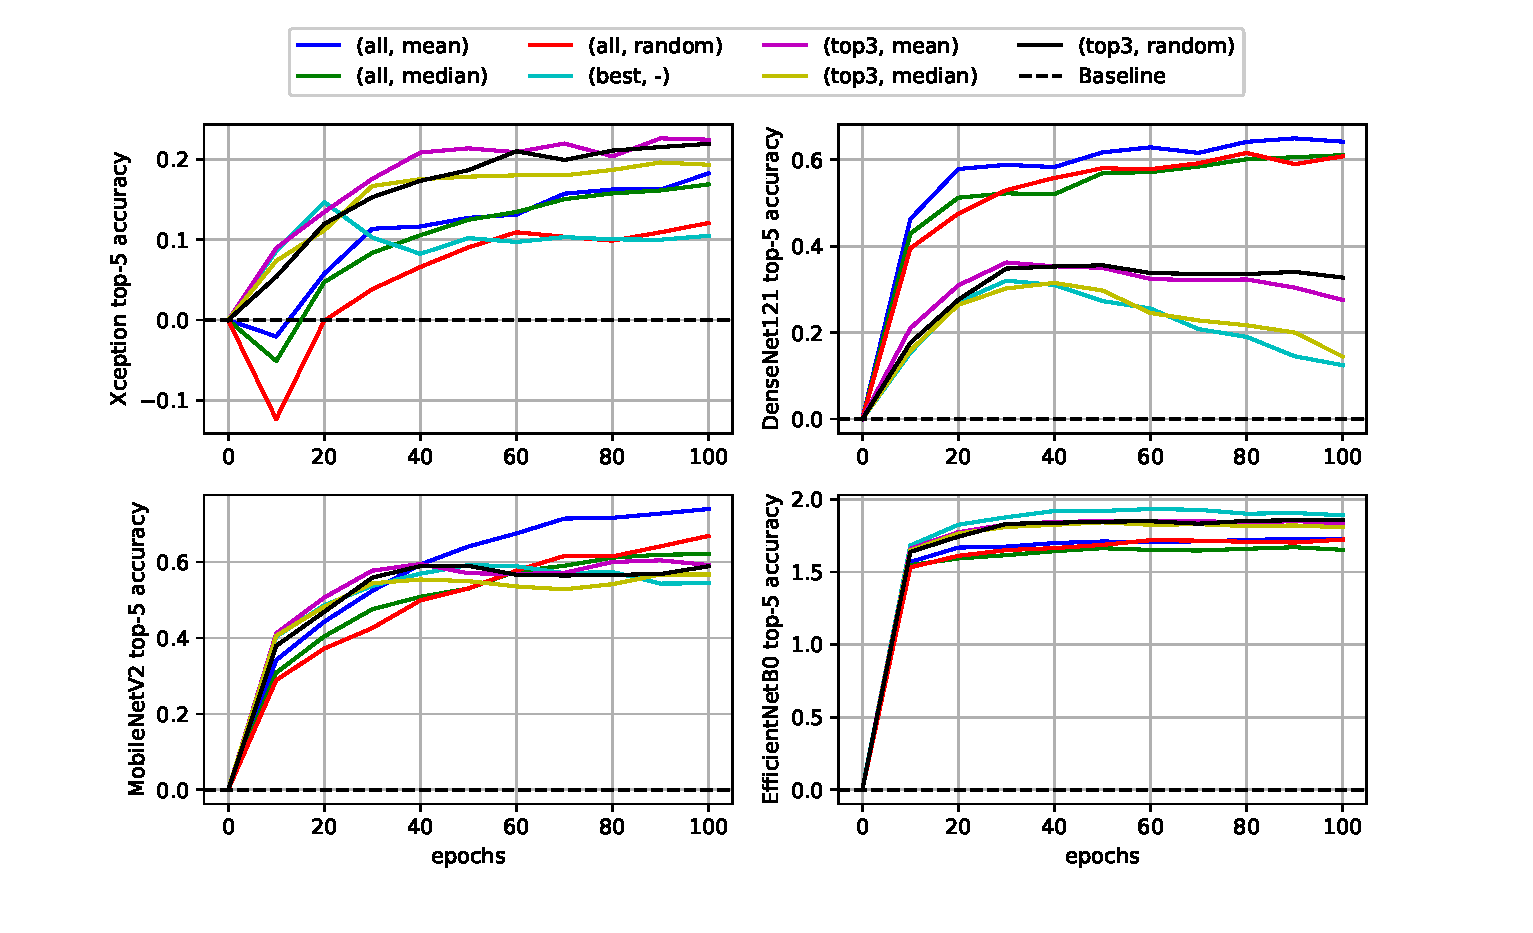
\includegraphics[width=1\linewidth]{distillation/images/top5_curves}
\caption{Absolute difference of top-5 accuracy with respect to the baseline. The x-axis represents the number of training iterations, and the tuples in the legend are expressed in the following format: (teachers set, combination method). The y-axis shows the absolute difference in performance with respect to the baseline.}
\label{fig:top5curves}
\end{figure}

Figures \ref{fig:top1curves} and \ref{fig:top5curves} show the training curves for all the cases. As it can be seen in the figures, although we reported the maximum accuracy achieved by each model, there are models for which the accuracy degrades more than the others if the model is trained for more epochs (for instance this is the general trend of the ``best'' teacher). We hypothesize that this phenomenon may be occurring because when several teachers are combined to build the distillation target, the complexity of the classification task increases and that has, in essence, a regularization effect.

In our experiments, we noticed that choosing a very small learning rate was crucial to achieve the performance reported. Higher learning rates ($\lambda=10^{-5}$ and  $\lambda=10^{-3}$) were tested leading to worse performances (sometimes even worse than the original pre-trained model). However we have not exhaustively studied this phenomenon due to the high resource requirements involved. We could associate this effect to catastrophic forgetting \autocite{French99}, which leads to overfitting to the transfer set when the learning rate is too big.




\section{Conclusions}  \label{sec:distillation_conclusions}
We have shown how by using simple knowledge distillation techniques the accuracy of the smallest pre-trained models increase in just few training epochs. This discovery opens potential new research lines towards more sophisticated teacher blending techniques or distillation methodologies. This can also motivate the research of novel training techniques, alternative or complementary to \textit{backpropagation}, as we empirically demonstrated that the pre-trained models still didn't reach their maximum capacity.



% Catastrophic forgetting is usually not a problem in pre-trained learning because the target task is different than the original task. It is not the case here.
% Incremental training: parameters of model i are used as initialization for parameters of model i+1

%!TEX root = ../thesis.tex
\chapter{End to end sales forecast with deep learning models} \label{ch:salesforecast}

\section{Overview}
Accurate and fast demand estimation is one of the key processes in supply chain that enables the precise execution of the corresponding downstream processes (inbound and outbound planning, inventory placement, network planning, etc). 

In this chapter, three alternatives are proposed to tackle the problem of forecasting the customer sales at day/store/item level using deep learning techniques and the \textit{Corporación Favorita} dataset, published as part of a \textit{Kaggle} competition. This chapter focuses on building a single end-to-end model, which is more convenient than a multi-model strategy from  energy efficiency and  model maintenance perspectives. The empirical results show how good performance can be achieved by using a simple \textit{sequence-to-sequence} architecture with minimal data pre-processing effort. Additionally, a training trick for making the model more time independent is described, and it showed evidences towards improving generalization over time. The proposed solution achieves a RMSLE of around 0.54, which is competitive with other more specific solutions to the problem proposed in the \textit{Kaggle} competition.

The development and usage of a standalone forecasting model that generalizes across time, locations and items requires less computational resources than fitting models for all the combinations. One of the main reasons is that a single global hyper-parameters search effort is required. In that search it is shown that for this particular case study simpler models (RNN-based) perform better or equal than large ones (transformer-based). In addition, evidences are found about the ineffectiveness of providing the models with historical information beyond the last 75 days, and this drastically reduces the amount of computation needed at inference time.

 All the code used in the experimentation part of this work has been made publicly available in a repository\footnote{\url{https://github.com/ivallesp/cFavorita}}.


\section{Introduction}
The retail industry economic activity is moving online. In the last years, e-commerce companies are gaining more and more adepts every day. \textit{E-Marketer} \autocite{emarketer2019, emarketer2020} reported consistent year on year growths in number of sales, being more than 13\% in the last 5 years in the US. The percentage of total sales in the US owned by e-commerce companies increased from 8,9\% to 14,5\% in 2020 \autocite{emarketer2019, emarketer2020}.

The continuously increasing demand requires the online industries to constantly improve their supply chain systems. This process entails multiple challenges such as: optimal inventory placement \autocite{graves2008}accurate network expansion \autocite{hossein2017}, precise inbound and outbound planning \autocite{kaipia2009}, etc. One of the most important wires that enables all those improvements is the ability to accurately forecast the customer demand for different products, locations and times \autocite{forslund2007}.

This study proposes several alternatives to solve the demand forecast problem in an end-to-end manner using deep learning techniques \autocite{Goodfellow2016}. The generalization power of these algorithms enables solving the problem using a single model for all the different locations and products time series, while other algorithms like the \textit{ARIMA} family of models \autocite{Hyndman2018} only can tackle one product-location time series at a time.

Two approaches are described in this chapter: (1) a \textit{sequence-to-sequence} (\textit{seq2seq} hereafter) architecture with product and (2) location conditioning and an adapted \textit{transformer} architecture for time series forecasting.


\subsection{Data} \label{sec:salesforecast_data}
The \textit{Corporación Favorita Grocery Sales} dataset  has been used to conduct this study \autocite{corporacionfavoritadataset2018}. \textit{Corporación Favorita}, an Ecuadorian company owner of multiple supermarkets across Latin America, released this dataset around 2017 as a \textit{Kaggle} competition to challenge the community to forecast their sales. It contains daily sales records for 4,400 unique items, in 54 different Ecuadorian stores from January 1st 2013 to August 15th 2017. Additional data provided along with the number of sales are described below.

\begin{itemize}
	\item \textit{ID variables}: date, store number and item number.
	\item \textit{Promotions}: a binary variable indicating if a given item, in a given store at a given time was on promotion.
	\item \textit{Store information}: location (city and state) and segment (type and cluster).
	\item \textit{Item information}: item family, class, and a binary variable indicating if the item is perishable.
	\item \textit{Transactions}: number of total sales for each store at each date.
	\item \textit{Oil price}: price of the oil on each date.
	\item \textit{Holidays and events}: dates, locations and types of holidays.
\end{itemize}

As it is usual in the supply chain organizations, the distribution of sales across products is very uneven (see Figure \ref{fig:tails}-left where the top 10\% of the products bring the 44\% of the sales). The same characteristic is observed in the case of the stores (see Figure \ref{fig:tails}-right where the top 10 stores bring 40\% of the sales). The sales for some products are very sparse: during the test period, the probability of having one or more sells for a given product in a given day is 47.6\%, which in practice means that more than half of the days in the time series will have value of zero.

\begin{figure}
	\centering
	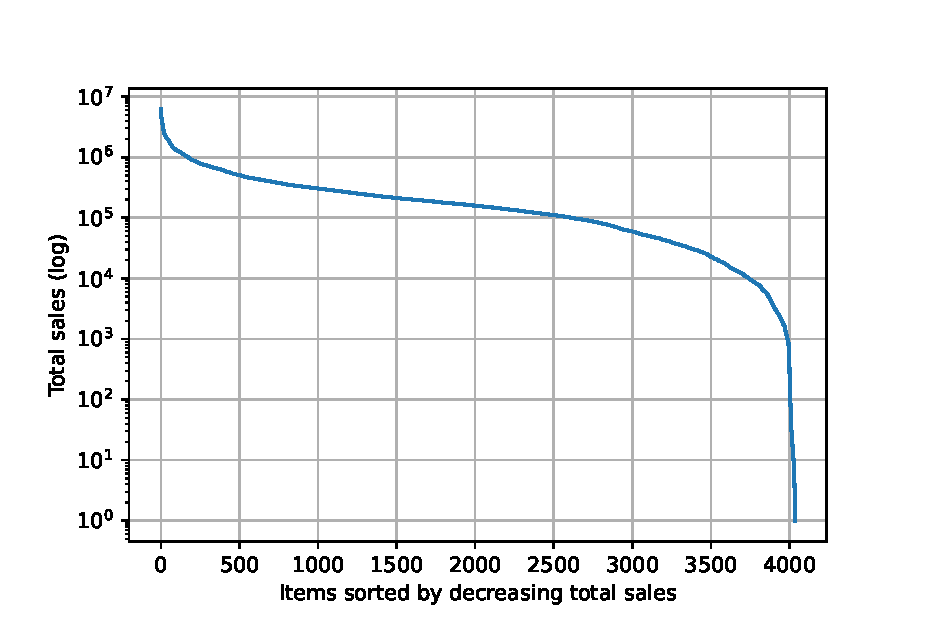
\includegraphics[width=0.48\linewidth]{salesforecast/images/items_tail_log}
	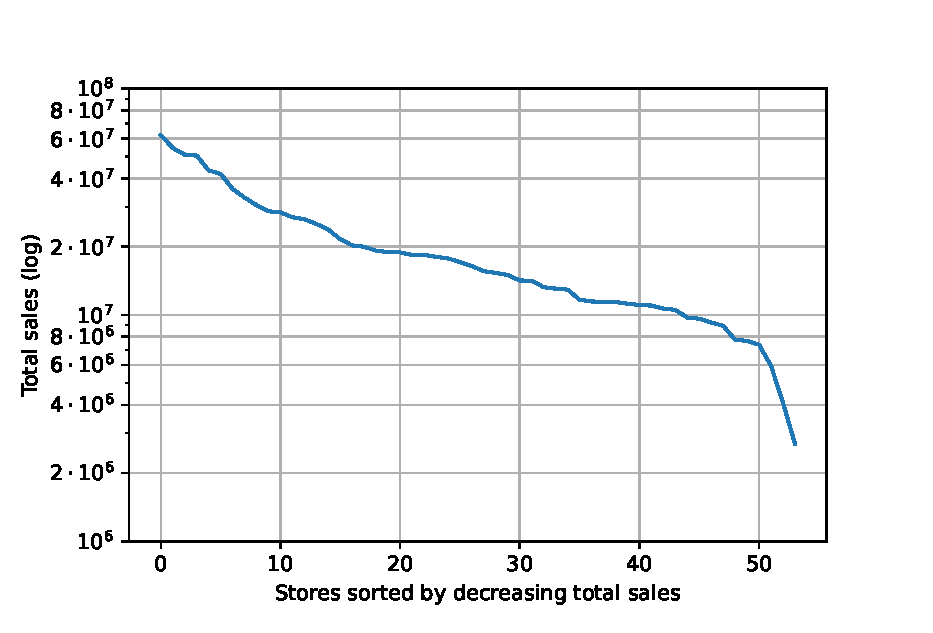
\includegraphics[width=0.48\linewidth]{salesforecast/images/stores_tail_log}
	\caption{Long tail distributions for items (left) and stores (right). Y axes represent total sells across all the history (around 5 years).}
	\label{fig:tails}
\end{figure}

As it can be noticed in Figure \ref{fig:timeseries}, the total sales show clear year on year trends as well as a very remarkable weekly seasonality (see Figure \ref{fig:timeseries_detail}). There is also a peak of sales at the end of each year.

 	\begin{figure}
 	\centering
 	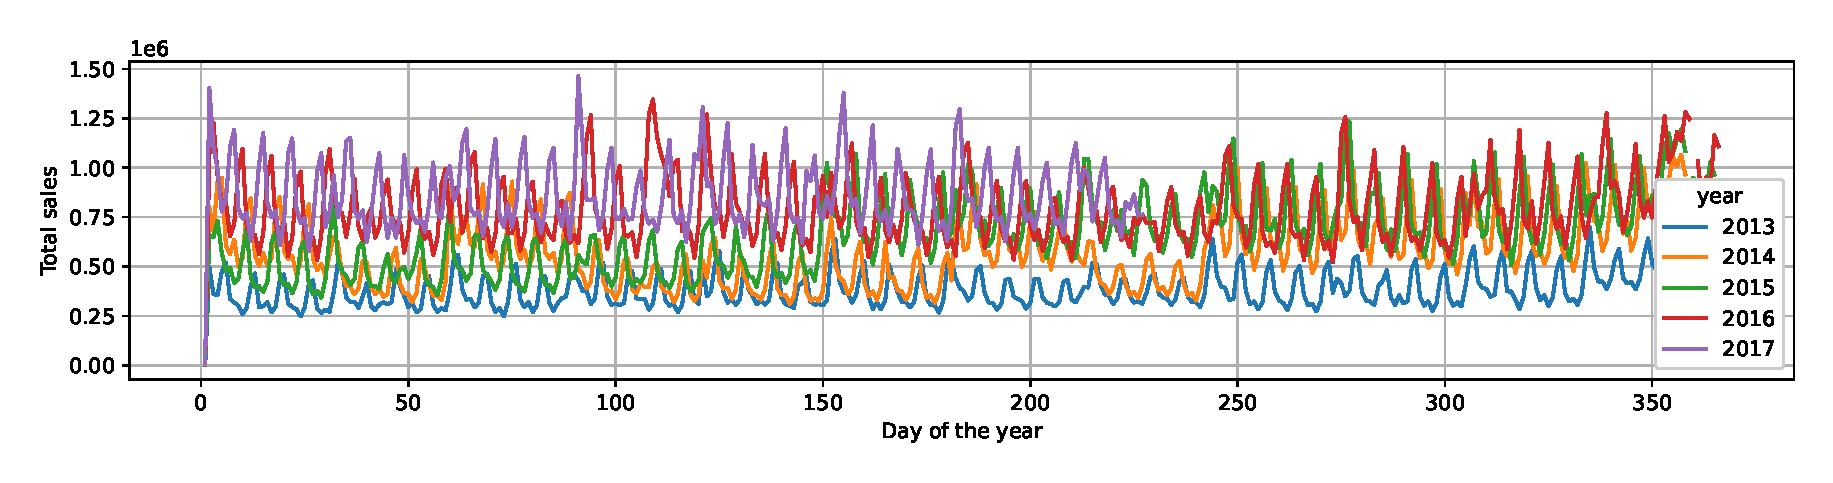
\includegraphics[width=1\textwidth]{salesforecast/images/timeseries}
 	\caption{Daily total sales for the 5 years included in the data.}
 	\label{fig:timeseries}
\end{figure}

\begin{figure}
	\centering
	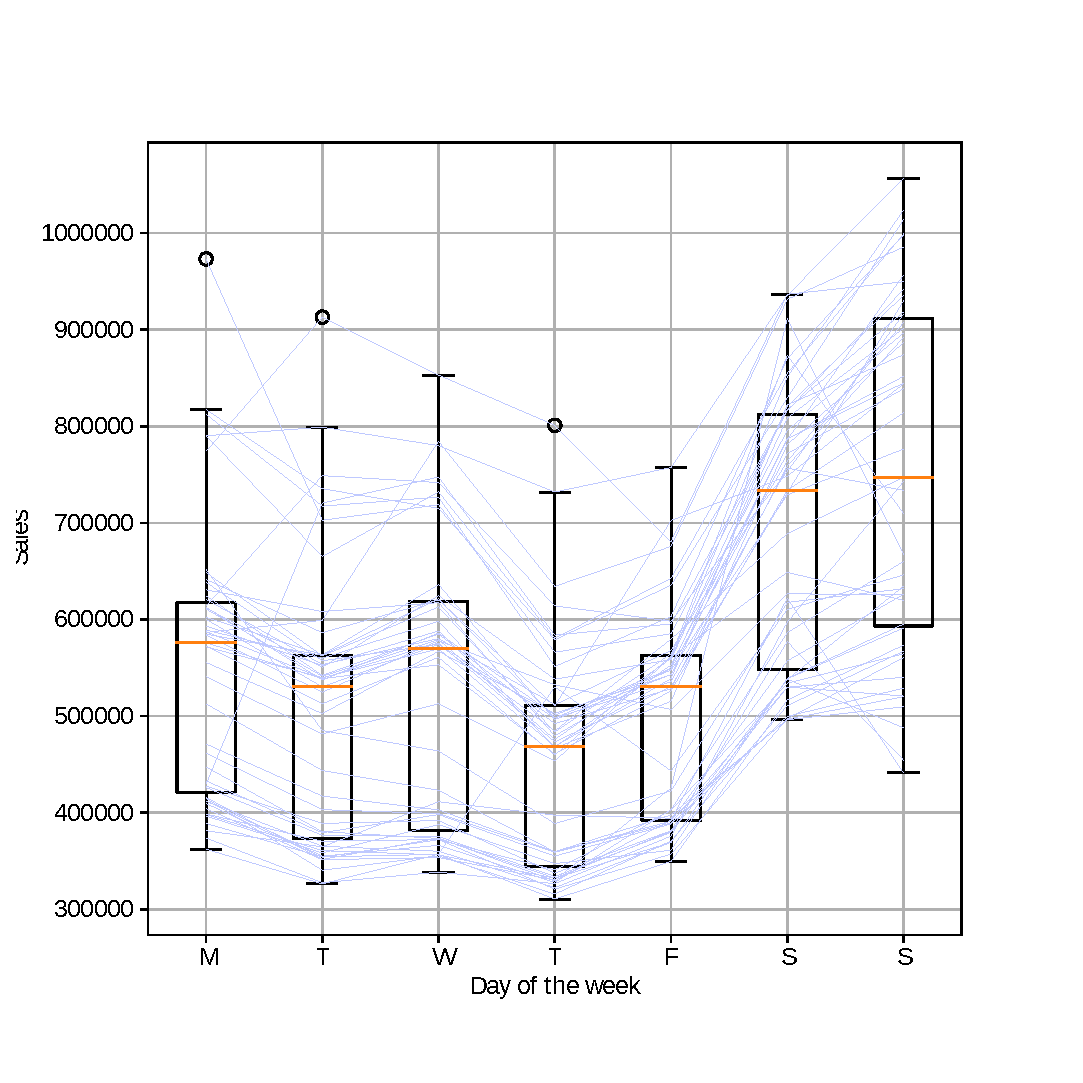
\includegraphics[width=0.6\textwidth]{salesforecast/images/timeseries_dow}
	\caption{Weekly pattern detail, including the 2014 sales.}
	\label{fig:timeseries_detail}
\end{figure}

The dataset does not contain records for items in days when there were zero unit sales. It also lacks information about the available inventory. These two facts together make the forecast effort more complicated, given that when there are zero sales of a given product in a store at a given date, it can be either because there was not available inventory, or because there was inventory but not demand (or both of them at the same time).

Estimating the actual demand of a retailer is not a straightforward task \autocite{Deep2019}. In this case, the quantity being forecasted is the number of sales. That would have an important implication in the demand estimation: the number of sales represent the demand as long as there exists available inventory. Hence, the quantity estimated by the machine learning model will be the demand bounded by the inventory $min(demand(i,s,d), inventory(i,s,d))$, where $i$, $s$ and $d$ are the inventory, the store and the date. There are techniques to correct the demand in these cases (e.g. \autocite{Bell2000}), however as the objective of this chapter is to build the forecast model, it is out of the scope to deal with that inconvenience.

\section{Previous work}	\label{sec:salesforecast_prevwork}
Several works have been published discussing the application deep learning techniques for demand and sales forecast in the supply chain environment. The authors of \autocite{Kilimci2019} use several \textit{multilayer perceptrons} (MLP) to build a unified forecast and compare it with more classical techniques. The main disadvantage of this approach is that it requires heavy feature engineering work, as the MLPs are not suitable to deal with time series. In a supply chain problem, this is not practical given the huge quantity of data normally available. In the work by \autocite{Talupula2018}, different deep learning architectures based on \textit{CNNs}, \textit{LSTMs} and MLPs are compared over an outbound demand forecast task, using data from a retailer. 

Similarly, \autocite{Helmini2019} compare a deep learning model based on LSTMs with peephole connections with more classical approaches using tree-based models.  The difference with the proposed approach is that it offers a set of flexible architectures capable to deal with multi-modal data more efficiently, while the models proposed in these works can only deal with time series. Furthermore, the proposed approach uses sequence-to-sequence modeling, which minimizes the error across all the predicted sequence. The authors of the aforementioned papers use a next-step prediction auto-regressive model, which only optimizes the error of the next time step.

However, only a few reports were found using this dataset for benchmarking. In \autocite{kechyn2018}, the authors used the \textit{WaveNet} \autocite{vanderoord2016} architecture to build an auto-regressive forecast. They achieved the 2nd position in the Kaggle competition that published the \textit{Corporación Favorita} data. The authors only show some charts summarizing their results, pointing to root mean squared weighted logarithmic errors (RMSWLE) of around 0.578 (see metrics definitions in section \ref{sec:salesforecast-results}. However, they do not give many details about the architecture used and the experimental framework. They also do not specify the period of time used to measure the errors. 

The authors of \autocite{Steves2018} used multiple classical techniques (historical average, ARIMA/SARIMA, seasonal-naïve and exponential smoothing) to forecast the daily sales. These techniques do not consider multiple sale points and products at the same time. They reach a minimum RMSWLE of 0.555. These solutions achieve competitive results, however, they require training one model per item and store (around 238,000 models), which is not a scalable approach for a production environment and constitute a non energy efficient alternative. The methods proposed in this chapter consist of a single model that is used over all the time periods, items and points of sale.

Other studies using the same dataset have been found: \autocite{wang2020c, Shaikhha2020, Schleich2019, Lim2019, Curtin2020, Malik2019, Kuleshov2018, Khamis2020}. Although some of them may be interesting for the supply chain goals, they deviate from the demand/sales forecast goal, hence they will not be summarized.

\section{Methods} \label{sec:salesforecast_methods}
The size of the dataset chosen (around $4\cdot10^8$ samples) enables the use of deep learning models. Two different neural architectures have been designed: a \textit{seq2seq} model and a \textit{transformer} model.

\subsection{Seq2seq}  % Cite Sutskever 2014

\begin{figure}
	\centering
	
\includegraphics[width=1\linewidth]{salesforecast/images/s2s}
	\caption{\textit{Seq2seq} architecture diagram. The left box shows the encoder, which takes the historical actual sales $y_i$ as input as well as other exogenous time-dependent features (i.e. oil price, holidays and events, transactions and promotions) denoted by $x_i$, and returns the hidden vector $h_t$ of the last recurrent module as output (aka \textit{context vector}). The middle of the figure shows the context conditioning module, which is the variation proposal over the original sequence-to-sequence proposal. This module receives the \textit{context vector} $h_t$ from the encoder module and concatenates it with static data $\hat{x}$ producing a conditioned context vector $\hat{h}_t = (h_t, \hat{x})$. Finally, on the right, the decoder module receives as initial state the conditioned context vector and provides the first recurrent cell with a \textit{go symbol} (constant input indicating the input of the decoded sequence). The decoder generates the sequence prediction in an auto-regressive way and $f$ is a stack of two fully-connected layers applied to each output of the decoder.}
	\label{fig:s2s}
\end{figure}

A sequence-to-sequence architecture (abbreviated as \textit{seq2seq}) is a model that is trained to map an input sequence to an output sequence (also known as sequence transduction), without any length restriction in both sides (input and output sequences can be of different length) \autocite{sutskever2014}. This architecture contains two main blocks: one encoder and one decoder. The encoder consists of a recurrent neural network which processes the input sequence, one sample at a time, condensing all the relevant input sequence information into a fixed length \textit{context vector}. This vector is usually the last hidden state of the encoder $\mathbf{h_t}$ \autocite{uday2019}. The decoder, also consisting of a recurrent neural network, generates the output sequence conditioned to the \textit{context vector}. Both modules are trained together to minimize an error term over the output.



For the purpose of the current objective, the original \textit{seq2seq} architecture has been slightly modified to condition the \textit{context vector} to a set of static (non time-dependent) features (see Figure \ref{fig:s2s} for a graphical representation of the architecture). To achieve that, the original context vector $\mathbf{h_t}$ has been concatenated with the static features (item and store embeddings and related features) and then passed into a feed-forward neural network with two hidden layers. The context conditioning module is an important part of the network because it allows the model to adapt the predictions to each product and store. The output of the feed-forward neural network has been used as the initial hidden state of the decoder. Other possible alternative would be to concatenate the static information along with every element of the input sequence. However the former approach was favoured given its benefit in terms of energy efficiency. The input of the first recurrent cell of the decoder is a special symbol that indicates the model that it is the first step of the output sequence. In this case, the special symbol is a vector containing all zeros.

The decoder module is an auto-regressive model trained to predict the immediate next step, i.e. the predicted value for time step $t$ is used as input for the prediction of time step $t+1$.



\subsection{Transformer}
\textit{Transformer} architectures were firstly published  in 2017 \autocite{vaswani2017}. This architecture removes the need to use recurrent neural networks by implementing attention and self-attention mechanisms \autocite{bahdanau2015}.  Like \textit{seq2seq} architectures, the transformers are able to map an input sequence to an output sequence, with potentially different lengths. Similar to the \textit{seq2seq} models, they also consist of two blocks: the encoder and the decoder; which function similarly as in the \textit{seq2seq} architecture.

The attention mechanism can be described as shown in equation \ref{eq:mhaconcat}. Where $Q$, $K$, $V$ stand for \textit{query}, \textit{key} and \textit{value}, respectively. These three pieces represent an analogy, introduced by \autocite{vaswani2017}, of the information retrieval systems where a \textit{query} is used in order to look for the matching \textit{key} (or the most similar one) and retrieving its \textit{value}. The attention mechanism working principle is similar to those systems (refer to section \ref{sec:transformer} for a deeper review of the attention mechanism). There are many possible differentiable similarity functions ($f$) that can be used \autocite{uday2019}. The authors of \autocite{vaswani2017} propose the Scaled dot product as similarity function, given that it is scaled so that different length sequences can be easily compared together. The Scaled dot product is defined in equation \ref{eq:scdotprod},  where $d_K$ represents the length of the key vector $K$. This version was adopted as it showed to work well in the initial transformer publication. The transformer architecture is described in detail in section \ref{sec:transformer}.

A slight modification has been performed over the original transformer, removing the \textit{softmax} operation of the output and only using the categorical embeddings for the categorical inputs. This is necessary in this case because the task is a regression and not a classification.

Following the information retrieval analogy and as illustrated in the figure \ref{fig:salesforecast_transformer}, there are two types of attention being used in this architecture.
\begin{itemize}
	\item \textit{encoder-encoder attention}: this is a form of self-attention that is used in the encoder module. In it, the \textit{query}, the \textit{key} and the \textit{value} come from the same time series.
	\item \textit{decoder-decoder masked attention}: also a form of self-attention with the particularity that the operation is forced to be causal, i.e. it only uses time steps from the past, the future ones are masked out. The \textit{query}, \textit{key} and \textit{value} come from the same time series.
	\item \textit{encoder-decoder attention}: this attention mechanism compares the decoder information with the encoder one, hence it is not self-attention. The \textit{query} comes from the decoder while the \textit{key} and \textit{value} are taken from the encoder output.
\end{itemize}

To train the \textit{transformer} architecture the \textit{teacher forcing} technique is used \autocite{williams1989, Goyal2016}. It consists of feeding the decoder with the target sequence, right-shifted by one sample so that the training can be done in one single calculation per batch. This technique is commonly used in auto-regressive models to improve the speed of training, and showed good results in the literature \autocite{vaswani2017}. 

At inference time, \textit{teacher forcing} is no longer available (because the future time steps of the time series are unknown) so auto-regression is used to compute the next steps recursively (i.e. the predicted sample is fed back to the input in order to predict the next sample). For a more detailed discussion of the transformer architecture, refer to section \ref{sec:transformer}.

% TODO: \usepackage{graphicx} required
\begin{figure}[h!]
   	\centering
   	\includegraphics[width=0.7\linewidth]{salesforecast/images/transformer}
   	\caption{Transformer architecture used to perform time series forecasting. In the diagram, the $||$ symbol stands for the concatenation operation, and similarly as in \autocite{vaswani2017}, $N_X$ represents the number of repetitions of the encoder and decoder blocks.}
   	\label{fig:salesforecast_transformer}
\end{figure}

\subsection{Random max time step trick}
At training time and with the aim of improving generalization over different periods of time, each \textit{mini-batch} has been constructed so that the maximum time step (the most recent one)  is drawn randomly from the time line. This trick allows the algorithm to learn a model that generalizes over different periods of time, preventing it to overfit to a single time span.

\section{Experiments and results} \label{sec:salesforecast_results}
\subsection{Setup}
The dataset provided has intentionally been minimally pre-processed as one of the goals of the current study is to provide a simple and flexible solution to the sales forecast problem. The most important transformation consisted of filling the zero sales records, as the dataset was provided without them. The numerical input variables have been standardized ($\mathbb{N}(0,1)$) while the categorical variables have been turned into \textit{one hot encoding} representations. The target variable has been scaled using a logarithmic transformation, as suggested by the authors of the dataset in the \textit{Kaggle} competition \autocite{corporacionfavoritadataset2018}. The ID variables corresponding to the store and the item have been used as an input to an embedding lookup layer to give the model the opportunity to learn store or item related information.

The model has been trained using daily data from January 1st 2013 to May 27th 2017, to produce daily forecasts of the next 16 days\footnote{this is not an arbitrary decision, the 16 days were chosen because that was the requirement in the \textit{Kaggle} competition. That choice would make sense for bi-monthly forecast publications, as it would be applicable for months with 28, 29, 30 and 31 days} from any present day. Data from  June 13th 2017 to June 28th 2017 have been used for validation purposes and the next 3 16-days time spans (June 29th to July 14th, July 15th to July 30th and July 31st to August 15th, referred subsequently as period 1, 2 and 3 respectively) have been used to test the performance of the algorithms.

The \textit{random max time step} has been constrained not to lay before October 29th 2013, to assure that the model has at least 300 days of history to learn from.

In the \textit{seq2seq} model all the history (from January 1st 2013) has been used as input.  In the \textit{transformer} model, given the quadratic computational complexity dependence on the length of the input sequence, the history had to be shortened to 200 days. In the spirit of fair comparison, an alternative \textit{seq2seq} version (referred subsequently as \textit{seq2seq trimmed}) has been trained using the 200 most recent time steps in every \textit{mini-batch}. To facilitate the interpretation of the results, two baselines have been included: \textit{random} and \textit{average}. The first one consists of measuring the accuracy of a naïve prediction built by randomly permuting the target variable. The second one consists of predicting the average of the target variable for all the instances.

\subsection{Results} \label{sec:salesforecast-results}

The results have been measured using the \textit{root mean squared logarithmic error} (\textit{RMSLE}, defined in equation \ref{eq:rmsle}), \textit{root mean squared weighted logarithmic error} (\textit{RMSWLE}, defined in equation \ref{eq:rmswle}, where the perishable items are given a weight of $1.25$, and $1.0$ to the rest),  and \textit{mean absolute logarithmic error} (\textit{MALE}, defined in equation \ref{eq:male}).

\begin{equation} \label{eq:rmsle}
RMSLE = \sqrt{ \frac{1}{N} \displaystyle\sum_{i=1}^N  \left(\log(\hat{y}_i + 1) - \log(y_i +1)  \right)^2  }
\end{equation}

\begin{equation} \label{eq:rmswle}
RMSWLE = \sqrt{ \frac{\displaystyle\sum_{i=1}^n w_i \left( \log(\hat{y}_i + 1) - \log(y_i +1)  \right)^2  }{\displaystyle\sum_{i=1}^n w_i}}
\end{equation}

\begin{equation} \label{eq:male}
MALE = \sqrt{ \frac{1}{N} \displaystyle\sum_{i=1}^N  \left|\log(\hat{y}_i + 1) - \log(y_i +1)  \right|  }
\end{equation}


In the previous equations, $\hat{y_i}$ represents the predicted sales,  $y_i$ represents the actual sales and $N$ is the total number of samples. The logarithmic component of the error metrics was introduced because different products at different shops have arbitrarily different demand levels. The usage of the logarithm scales the unit sales distribution and makes the whole problem easier to measure. A natural logarithm has been used along all this chapter. The \textit{RMSWLE} error metric has been introduced for easier comparison and benchmarking with future studies.

Figure \ref{fig:performance_evolution} shows how the errors evolve in every epoch. Figure \ref{fig:stores_items_performance} decomposes the error at store and item level, in order to show in detail how the errors vary along these dimensions. Finally, Figures \ref{fig:ts_log} and \ref{fig:ts_lin} show examples of actual and forecasted time series in log and linear scales, respectively.

\begin{figure}[h!]
	\centering
	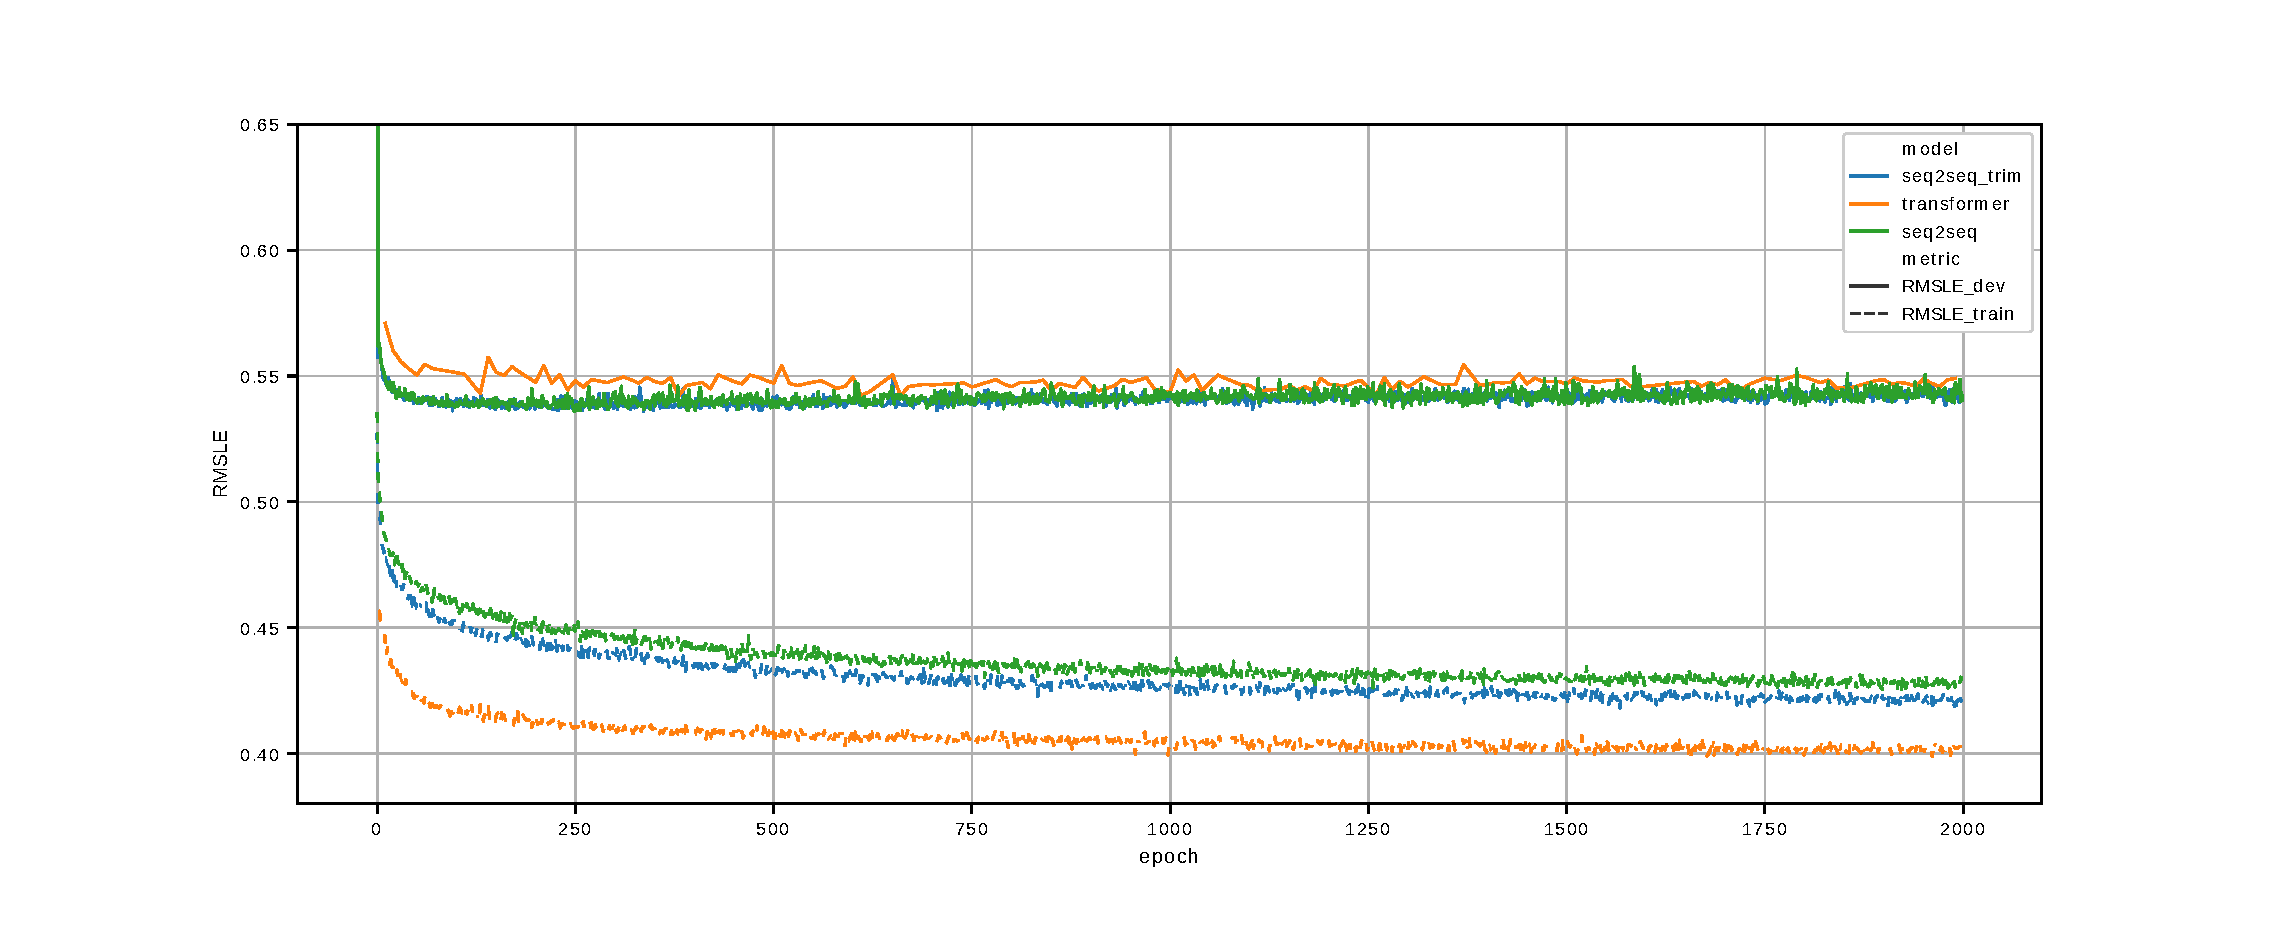
\includegraphics[width=1\linewidth]{salesforecast/images/evolution}
	\caption{Evolution of the train and validation (dev) error during the process of training, for all the models.}
	\label{fig:performance_evolution}
\end{figure}

 \begin{figure}[h!]
	\centering
	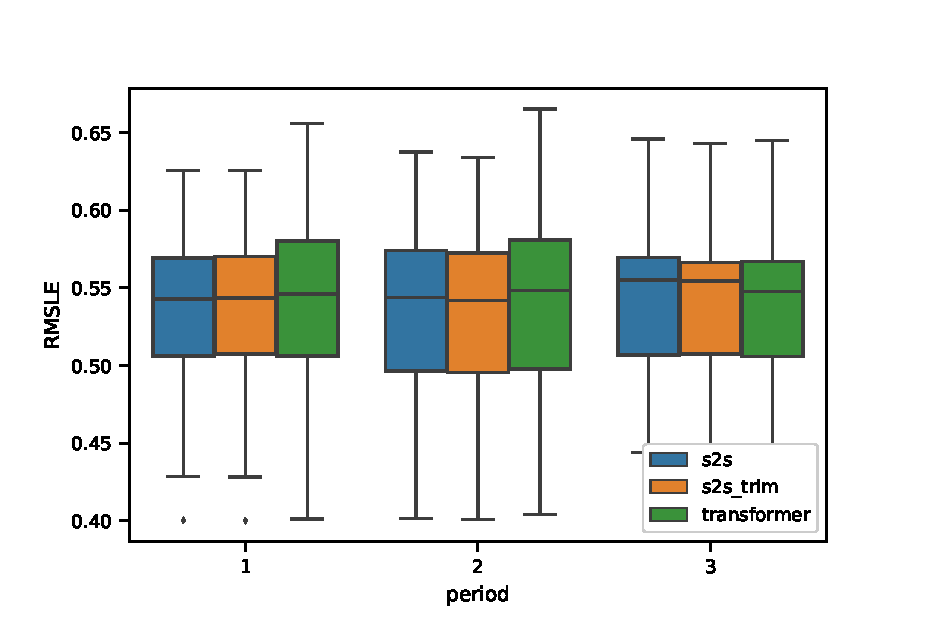
\includegraphics[width=0.48\linewidth]{salesforecast/images/rmsle_storewise}
	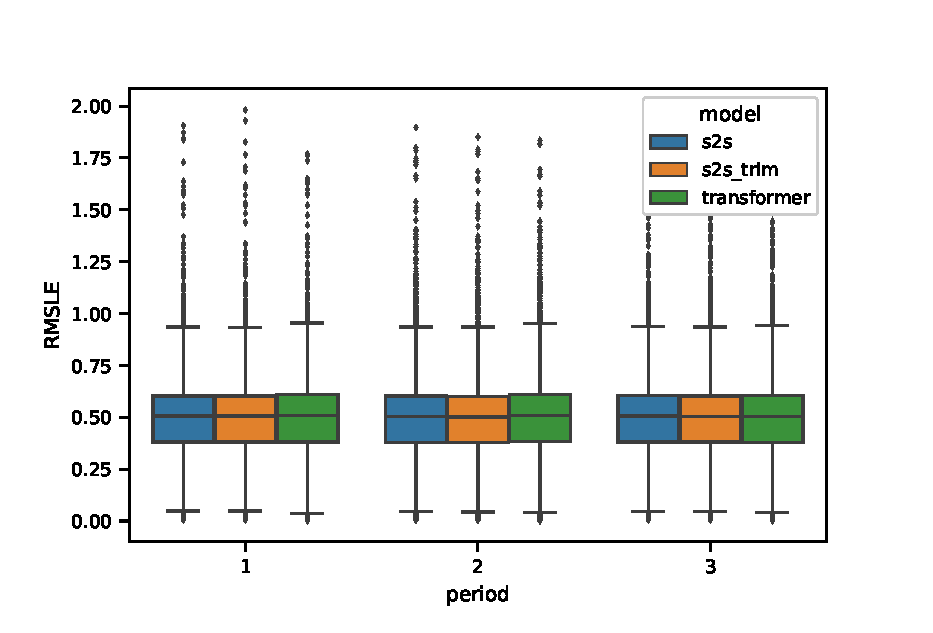
\includegraphics[width=0.48\linewidth]{salesforecast/images/rmsle_itemwise}
	\caption{Distribution of the error across stores (left) and accross items (right) for every model  and for the three different test periods used.}
	\label{fig:stores_items_performance}
\end{figure}

\begin{figure}
	\centering
	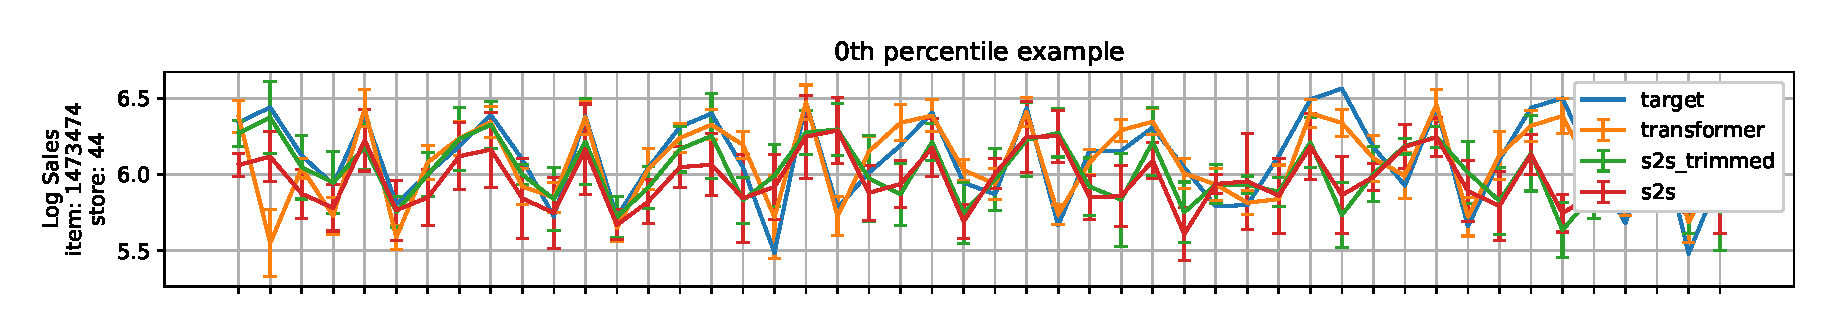
\includegraphics[width=1\linewidth]{salesforecast/images/sample_0_log}
	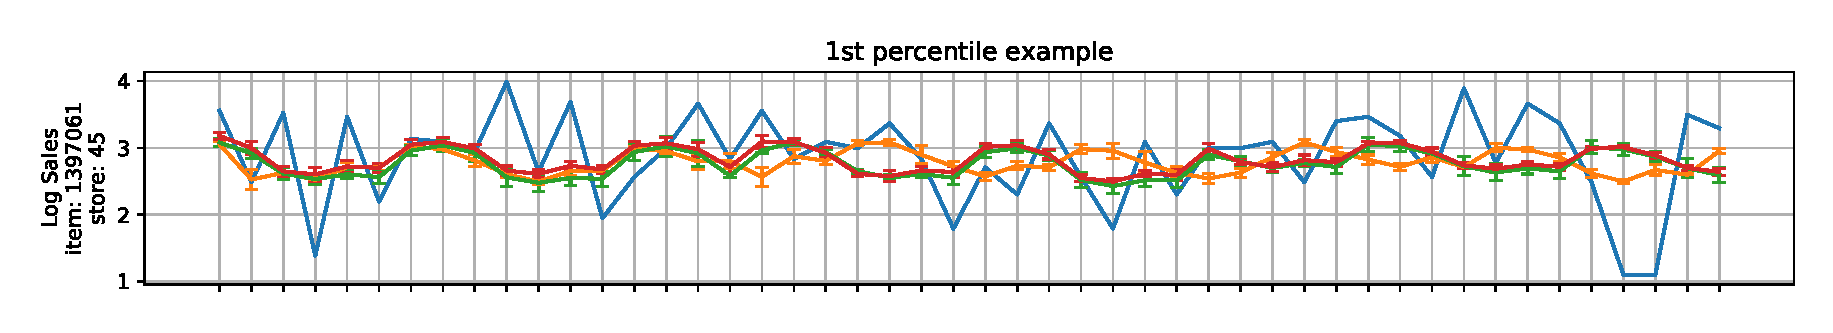
\includegraphics[width=1\linewidth]{salesforecast/images/sample_1_log}
	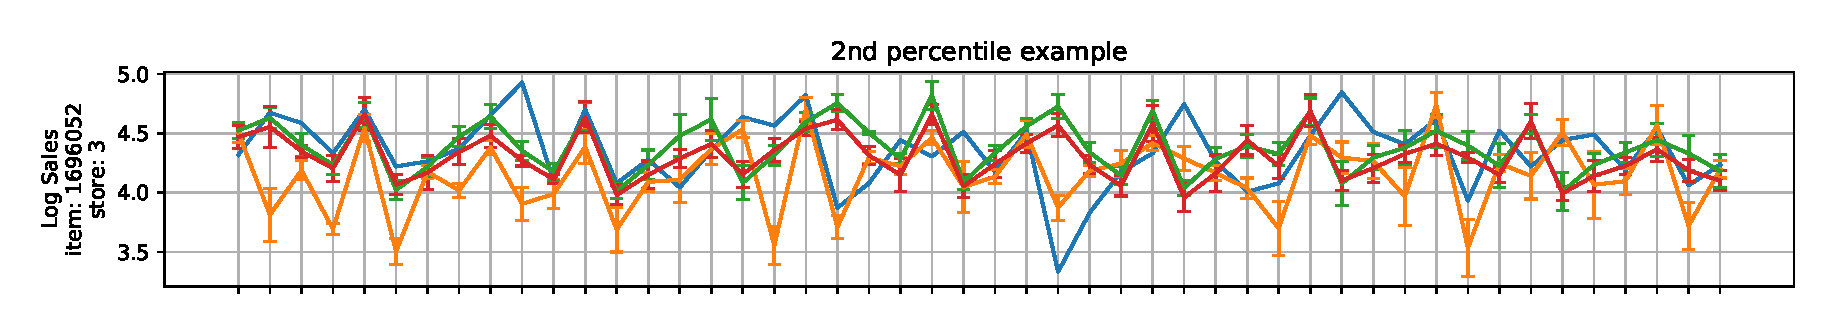
\includegraphics[width=1\linewidth]{salesforecast/images/sample_2_log}
	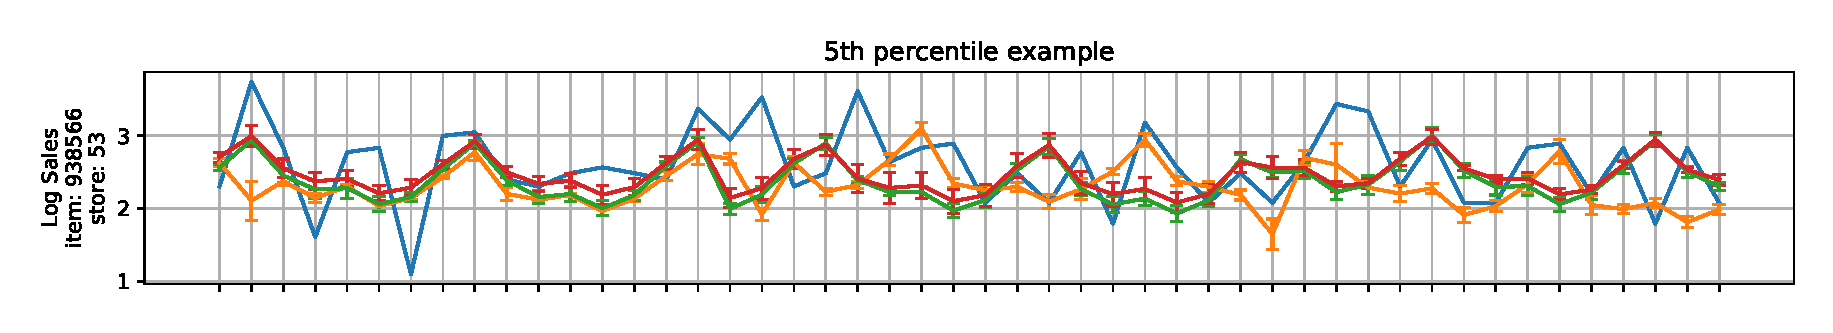
\includegraphics[width=1\linewidth]{salesforecast/images/sample_3_log}
	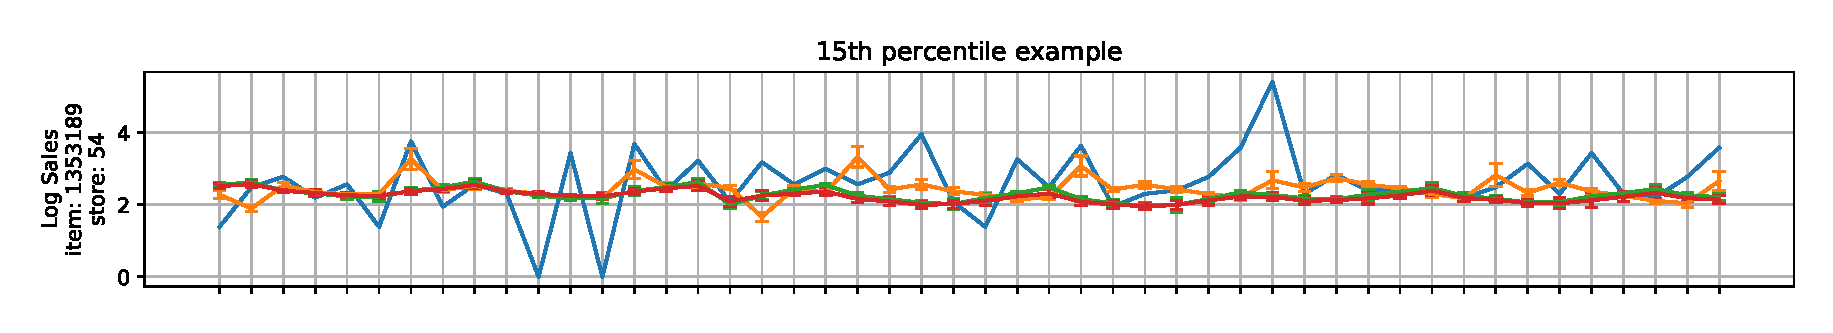
\includegraphics[width=1\linewidth]{salesforecast/images/sample_4_log}
	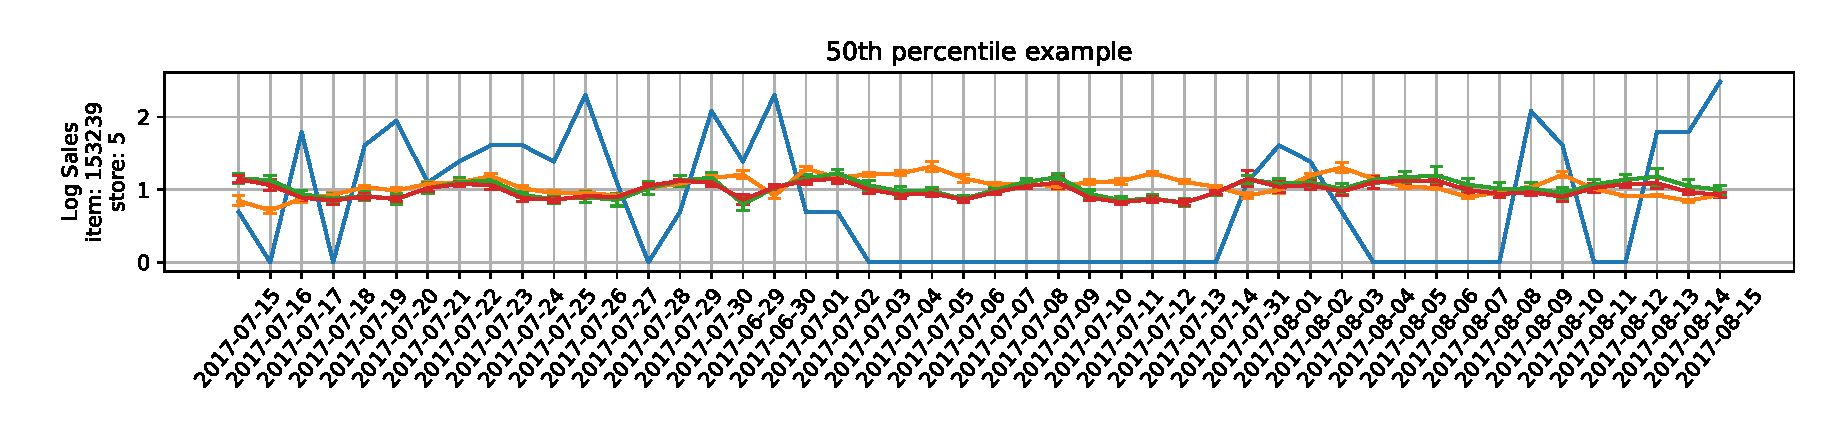
\includegraphics[width=1\linewidth]{salesforecast/images/sample_5_log}
\caption{Actual and forecasted sales in log scale for six examples of store-item combinations representing the 0th (best prediction), 1st, 2nd, 5th 15th and 50th percentiles of RMSLE (relative to the target variable average) from top to bottom. The three test periods have been concatenated along the X axis. The error bars show the standard deviation across the 5 runs. }
	\label{fig:ts_log}
\end{figure}

\begin{figure}
\centering
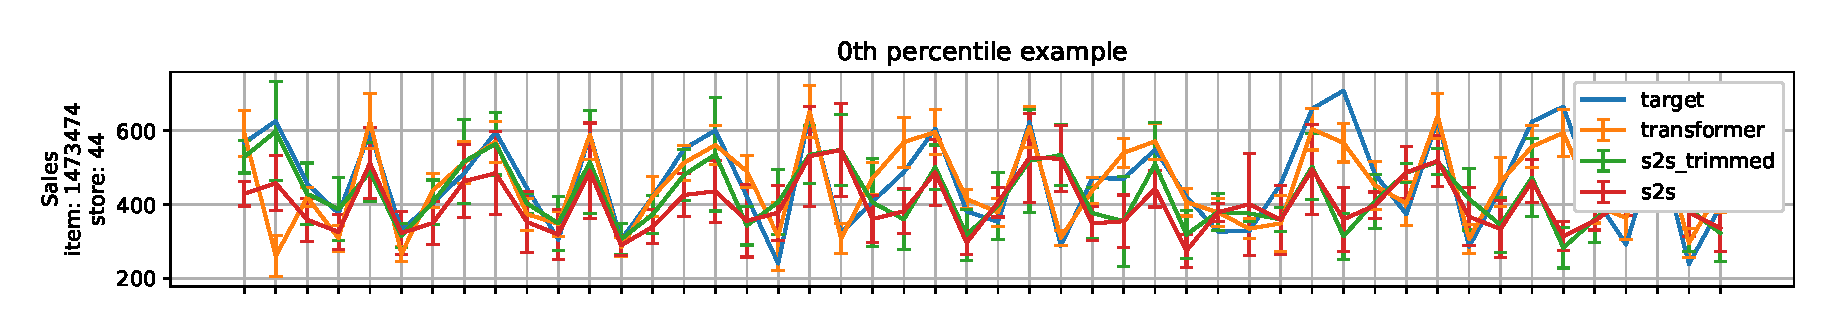
\includegraphics[width=1\linewidth]{salesforecast/images/sample_0_lin}
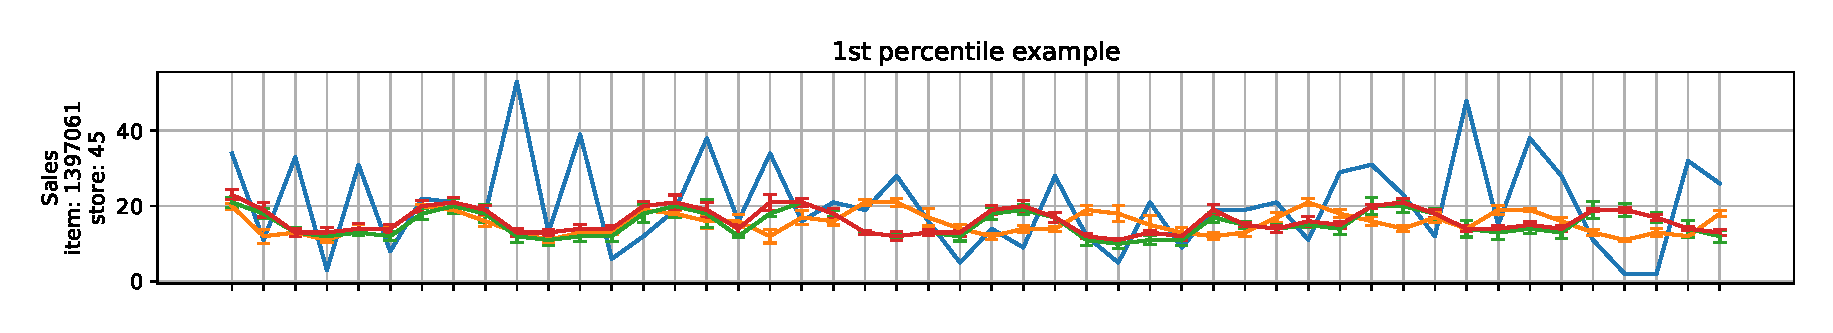
\includegraphics[width=1\linewidth]{salesforecast/images/sample_1_lin}
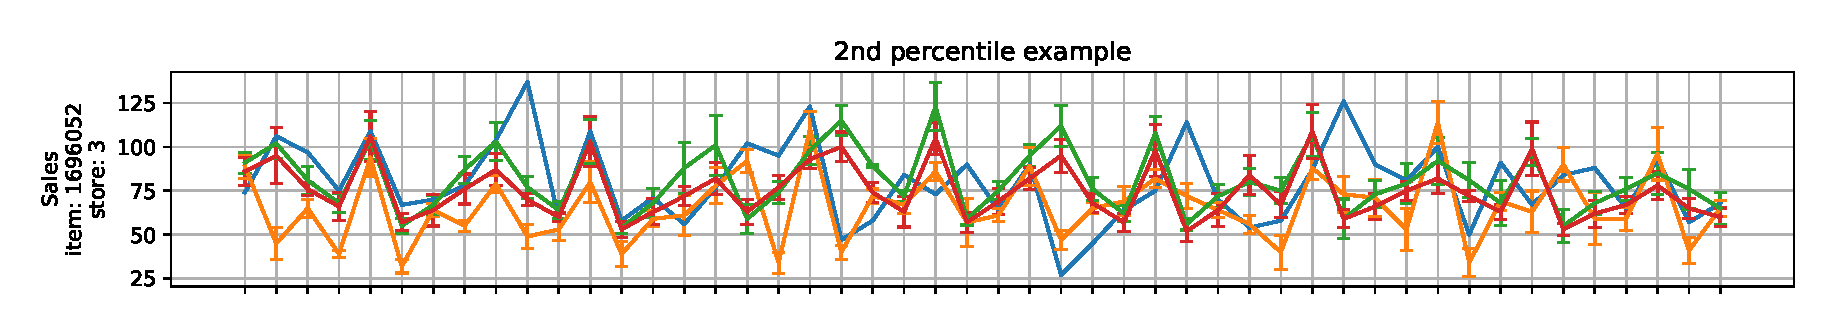
\includegraphics[width=1\linewidth]{salesforecast/images/sample_2_lin}
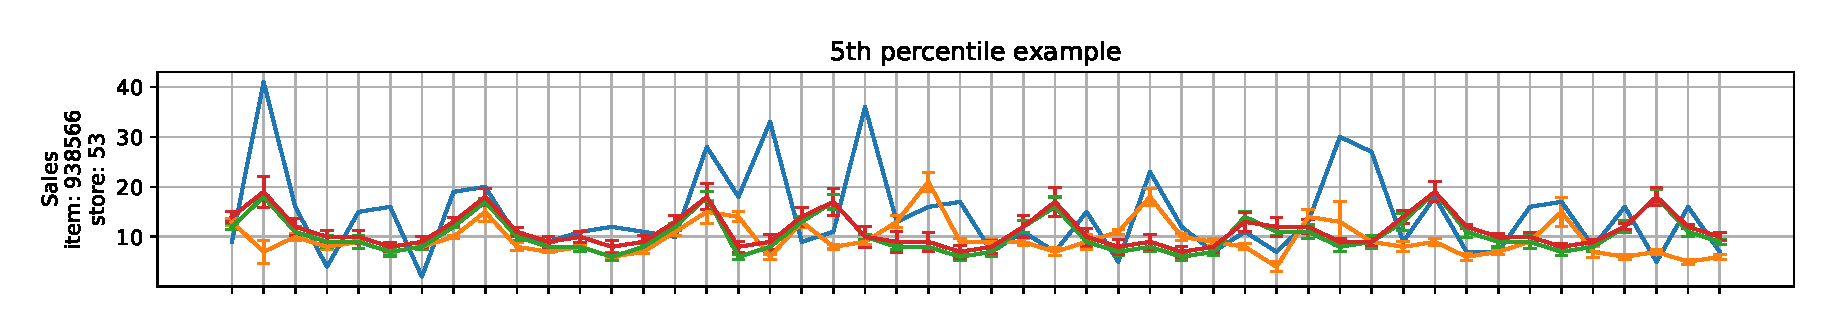
\includegraphics[width=1\linewidth]{salesforecast/images/sample_3_lin}
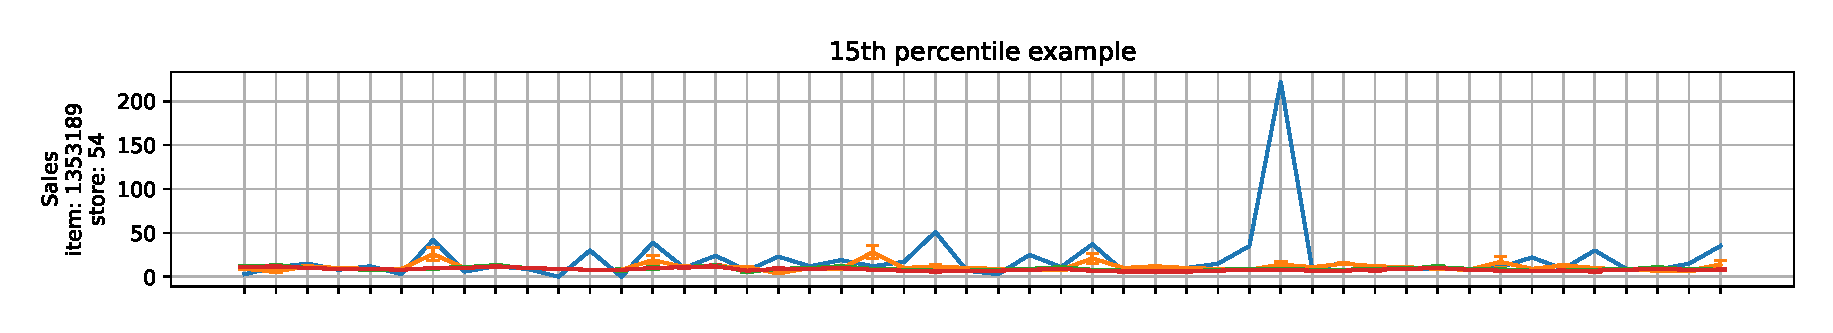
\includegraphics[width=1\linewidth]{salesforecast/images/sample_4_lin}
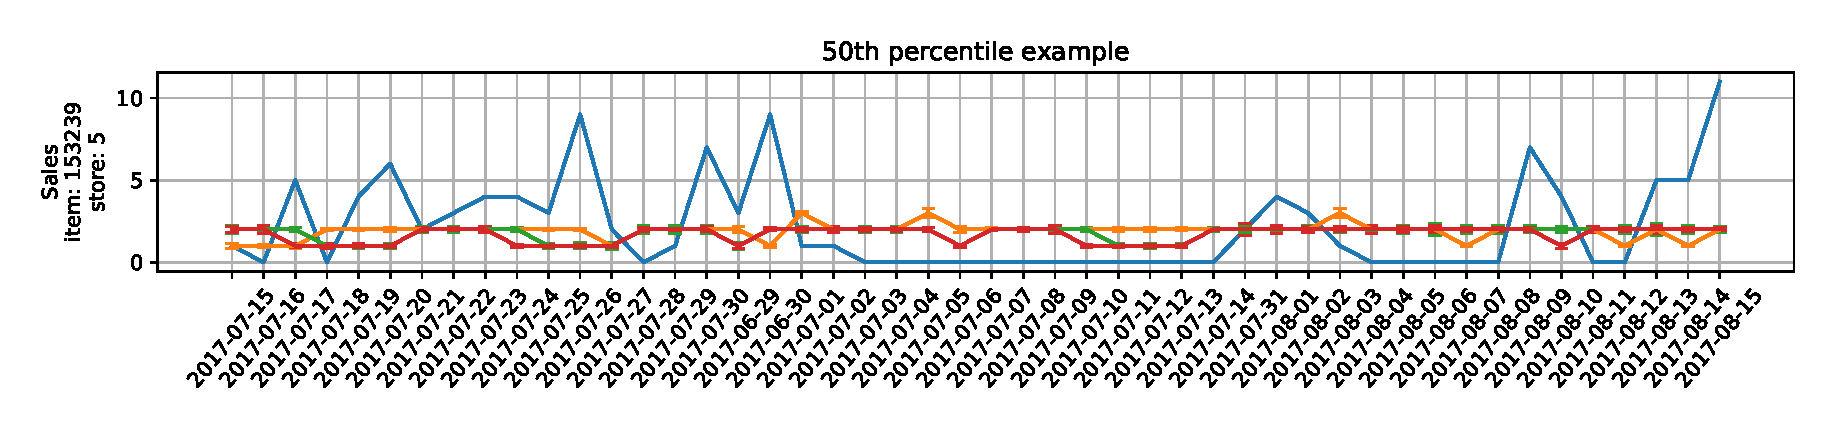
\includegraphics[width=1\linewidth]{salesforecast/images/sample_5_lin}
\caption{Actual and forecasted sales in linear scale for six examples of store-item combinations representing the 0th (best prediction), 1st, 2nd, 5th 15th and 50th percentiles of RMSLE (relative to the target variable average) from top to bottom. The three test periods have been concatenated along the X axis. The error bars show the standard deviation across the 5 runs. Some of the examples are better viewed in log-scale (refer to figure \ref{fig:ts_log}).}
\label{fig:ts_lin}
\end{figure}

As shown in figure \ref{fig:stores_items_performance}, the performance is very similar across models. A numerical comparison of the errors obtained for every model is presented in Table \ref{tab:salesforecast_results}. Additionally, a deeper daily analysis is provided in Figure \ref{fig:dailyerror}. From these figures, it can be noticed that the error is not distributed uniformly across products, stores and time.
%More details about the model performance are included in the appendix, including error distribution across different stores and products, and a set of figures showing how the predicted time series match the actual values.

Table \ref{tab:salesforecast_results} shows that the three models perform similarly. However, the daily figures show that the transformer error has more variability around the second and fourth day of forecast. This may be due to the fact that the model has been trained using \textit{teacher forcing} \autocite{williams1989, Goyal2016}, and at inference time, an auto-regressive strategy has been used to compute the forecasted sales. This may cause distribution shifts that impact the quality of the forecast.  Besides, the \textit{seq2seq} models were much faster at training and inference time. This is due to the quadratic complexity dependence on the sequence length in the \textit{transformer} architecture; in \textit{seq2seq} it is linear. The simplest model (\textit{seq2seq trimmed}) was the fastest of the three alternatives, with no noticeable decrease in performance, either in the general picture or in the daily figures.

\begin{table}[h]
\scriptsize
\caption{Results of the models trained for three different time spans. All the models have been trained five times to reduce the effect of different random initialization. The errors are represented as mean $\pm$ standard deviation, across the five runs. The rows corresponding with the models that achieved the lowest RMSLE have been highlighted in bold. At the bottom of the table two benchmark metrics extracted from the previous works have been included. However, the authors of those works do not clearly specify the period of time used to measure the results, hence they should be used only as a reference.}
	\label{tab:salesforecast_results}
	\centering
	\begin{tabular}{lllll}
		\hline
		Period    & Model                     & RMSLE                          & RMSWLE                         & MALE                           \\ \hline
		1         & \textbf{Seq2seq}          & $ \mathbf{0.5380 \pm 0.0016} $ & $ \mathbf{0.5376 \pm 0.0016 }$ & $  \mathbf{0.3450 \pm 0.0024}$ \\
         & Seq2seq trimmed           & $ 0.5381 \pm 0.0008 $          & $ 0.5377 \pm 0.0008 $          & $ 0.3442 \pm 0.0008 $          \\
         & Transformer               & $ 0.5439 \pm 0.0024 $          & $ 0.5436 \pm 0.0023 $          & $ 0.3386 \pm 0.001 $           \\
         & Baseline: random          & $ 1.474 \pm 0.0003 $           & $ 1.4795 \pm 0.0003 $          & $ 1.0691 \pm 0.0002 $          \\
         & Baseline: average         & $ 1.0422$                      & $ 1.05$                        & $ 0.8744$                      \\ \hline
		2         & Seq2seq                   & $ 0.5431 \pm 0.0014 $          & $ 0.5421 \pm 0.0013 $          & $ 0.3475 \pm 0.0012 $          \\
         & \textbf{Seq2seq trimmed } & $ \mathbf{0.5413 \pm 0.0019} $ & $ 0.\mathbf{5403 \pm 0.0018 }$ & $ \mathbf{0.3444 \pm 0.0012} $ \\
         & Transformer               & $ 0.5495 \pm 0.0021 $          & $ 0.5486 \pm 0.0021 $          & $ 0.3415 \pm 0.0012 $          \\
         & Baseline: random          & $ 1.4649 \pm 0.0002 $          & $ 1.4702 \pm 0.0002 $          & $ 1.0577 \pm 0.0003 $          \\
         & Baseline: average         & $ 1.0358$                      & $ 1.0433$                      & $ 0.8655$                      \\ \hline
		3         & Seq2seq                   & $ 0.544 \pm 0.0021 $           & $ 0.5431 \pm 0.0021 $          & $ 0.3502 \pm 0.0028 $          \\
         & Seq2seq trimmed           & $ 0.5423 \pm 0.0015 $          & $ 0.5414 \pm 0.0016 $          & $ 0.3481 \pm 0.0017 $          \\
         & \textbf{Transformer}      & $ \mathbf{0.5414 \pm 0.0015} $ & $ \mathbf{0.5407 \pm 0.0014} $ & $ \mathbf{0.3366 \pm 0.0012} $ \\
         & Baseline: random          & $ 1.4555 \pm 0.0002 $          & $ 1.4606 \pm 0.0002 $          & $ 1.0517 \pm 0.0002 $          \\
         & Baseline: average         & $ 1.029$                       & $ 1.0363 $                     & $ 0.8616$                      \\ \hline
		Benchmark & \autocite{kechyn2018}         & -                              & 0.5780                          & -                              \\
		Benchmark & \autocite{Steves2018}         & -                              & 0.5550                          & -                              \\ \hline
	\end{tabular}
\end{table}


\begin{figure}
\centering
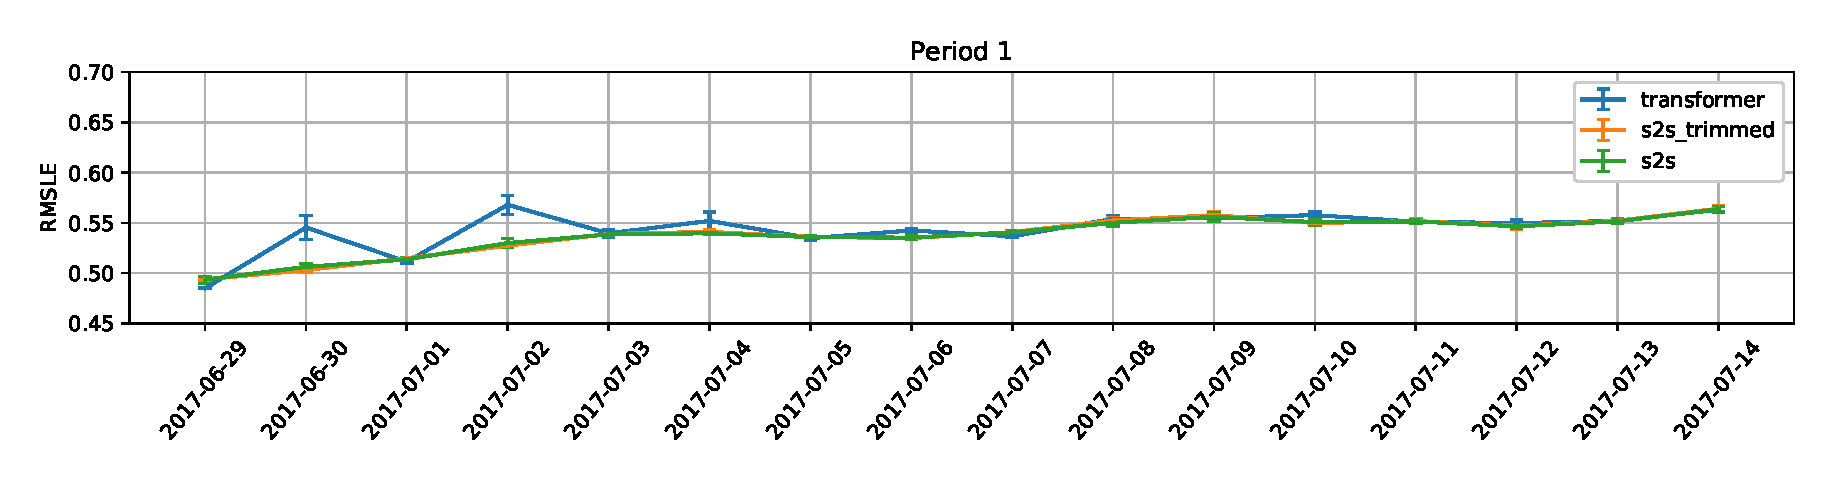
\includegraphics[width=1\linewidth]{salesforecast/images/lag3_daily_error}
\includegraphics[width=1\linewidth]{salesforecast/images/lag2_daily_error}
\includegraphics[width=1\linewidth]{salesforecast/images/lag1_daily_error}
\caption{Daily \textit{RMSLE} for the three test periods (in chronological order, from top to bottom). The error bars shown in the figures represent the standard deviation of the three runs. Despite the error spikes in the 2nd day of the forecast, an ANOVA test shows non-significant differences between the average performance of the three models (with the following p-values: 0.0947, 0.1823 and 0.6181 for periods 1, 2 and 3, respectively). }
\label{fig:dailyerror}
\end{figure}


\subsection{Ablation study}
This subsection contains an analysis of the effect of two core pieces of the proposed architecture: the \textit{random max time step trick} and the length of the  input sequences in the \textit{seq2seq trimmed} model.

\subsubsection{Random max time step trick}
The \textit{seq2seq trimmed} model is retrained without the \textit{random max time step trick}. Table \ref{tab:salesforecast_results_notrick} summarizes the errors obtained at the best iteration of each model, averaged across five repeated runs. From the results one can conclude that when the \textit{random max time step trick} is used, the model achieves significantly superior performance. This is due to the fact that randomizing the max time step helps the model to capture behaviors of the target signal at different times. Figure \ref{fig:traincurvesnotrick}, shows the training curves when the trick is used and when it is not used, suggesting that the trick may also act as a regularization technique, as the model is much less prone to overfitting when the trick is used.

	\begin{table}[h]
	\footnotesize
	\caption{Results of the models trained with and without the \textit{random max time step trick}. All the models have been trained five times to reduce the effect of different random initialization. The errors are represented as mean $\pm$ standard deviation, across the five runs. The rows corresponding with the models that achieved the lowest RMSLE have been highlighted in bold.}
	\label{tab:salesforecast_results_notrick}
	\centering
	\begin{tabular}{lllll}
		\hline
		Period & Trick/No trick             & RMSLE                 & RMSWLE                & MALE                  \\ \hline
		1 & Trick   & $ \mathbf{0.5381 \pm 0.0008} $ & $ \mathbf{0.5377 \pm 0.0008} $ & $ \mathbf{0.3442 \pm 0.0008} $ \\
		& No trick & $ 0.6077 \pm 0.0055 $  &  $ 0.6073 \pm 0.0054 $  &  $ 0.4037 \pm 0.0171 $ \\
		\hline
		2 & Trick  & $ \mathbf{0.5413 \pm 0.0019} $ & $ \mathbf{0.5403 \pm 0.0018} $ & $ \mathbf{0.3444 \pm 0.0012} $ \\
		& No trick & $ 0.5895 \pm 0.0042 $  &  $ 0.5886 \pm 0.0042 $  &  $ 0.3892 \pm 0.0216 $ \\
		\hline
		3 & Trick  & $ \mathbf{0.5423 \pm 0.0015} $ & $ \mathbf{0.5414 \pm 0.0016} $ & $ \mathbf{0.3481 \pm 0.0017} $ \\
		& No trick & $ 0.5929 \pm 0.0127 $  &  $ 0.5922 \pm 0.0125 $  &  $ 0.3938 \pm 0.0318 $ \\
		\hline
	\end{tabular}
\end{table}

% TODO: \usepackage{graphicx} required
\begin{figure}[h!]
	\centering
	\includegraphics[width=0.7\linewidth]{salesforecast/images/train_curves_notrick}
	\caption{Training and validation MALE curves of the \textit{seq2seq trimmed} when using the \textit{random max time step trick} and when disabling it.}
	\label{fig:traincurvesnotrick}
\end{figure}

\subsubsection{Input sequences length}
As showed in the Table \ref{tab:salesforecast_results}, the \textit{seq2seq} model can be further simplified by trimming the length of the input sequences. This subsection studies the minimum length of the input sequence without significant performance degradation. For that, the \textit{seq2seq} model was retrained with different input sequence lengths to determine where is the optimum. The Table 		\ref{tab:salesforecast_results_ablation_length} shows the results of the model with the full sequences, and with sequences trimmed to 200, 75, 10, 1 and 0 time steps (where 0 time steps means not using any input sequence information at all, only static features). 

The results show that it is possible to reduce the sequence lengths to up to 75 time steps without losing performance (and even slightly improving the generalization). Further reductions to 10 and 1 time steps start showing performance degradation. When not using input sequences (length=0) the performance degrades notably, as compared to using only one time step. The most plausible hypothesis is that this happens because the model needs some reference level of number of sales per product to produce accurate forecasts.

	\begin{table}[h]
	\footnotesize
	\caption{Results of the \textit{seq2seq} models trained with different input sequence lengths. All the models have been trained five times to reduce the effect of different random initialization. The errors are represented as mean $\pm$ standard deviation, across the five runs. The rows corresponding with the models that achieved the lowest RMSLE have been highlighted. An asterisk is added to the experiments where the metric is significantly different than the full sequence error (as per a two-tail T-test with $\alpha=0.05$)}
	\label{tab:salesforecast_results_ablation_length}
	\centering
	\begin{tabular}{lllll}
		\hline
		Period & Sequence length & RMSLE                           & RMSWLE                         & MALE                           \\ \hline
		1      & Full            & $ 0.5380 \pm 0.0016 $           & $ 0.5376 \pm 0.0016 $          & $  0.3450 \pm 0.0024$          \\
      & 200             & $ 0.5381 \pm 0.0008 $           & $ 0.5377 \pm 0.0008 $          & $ 0.3442 \pm 0.0008 $          \\
      & \textbf{75}     & $ \mathbf{0.5372 \pm 0.0016} $  & $ \mathbf{0.5369 \pm 0.0016} $ & $ \mathbf{0.3458 \pm 0.0034} $ \\
      & 10              & $ 0.5452 \pm 0.0008 *$          & $ 0.5447 \pm 0.0009 *$         & $ 0.3478 \pm 0.0017 $          \\
      & 1               & $ 0.5812 \pm 0.0042 *$          & $ 0.5807 \pm 0.0042 *$         & $ 0.3795 \pm 0.0029 *$          \\
      & 0               & $ 0.8411 \pm 0.0016 *$          & $ 0.8453 \pm 0.0015 *$         & $ 0.5408 \pm 0.0028 *$          \\ \hline
		2      & Full            & $ 0.5431 \pm 0.0014 $           & $ 0.5421 \pm 0.0013 $          & $ 0.3475 \pm 0.0012 $          \\
      & 200             & $ 0.5413 \pm 0.0019 $           & $ 0.5403 \pm 0.0018 $          & $ 0.3444 \pm 0.0012 *$          \\
      & \textbf{75}     & $ \mathbf{0.5400 \pm 0.0010}* $ & $ \mathbf{0.5392 \pm 0.001}* $ & $ \mathbf{0.3458 \pm 0.0009} $ \\
      & 10              & $ 0.5510 \pm 0.0049 *$          & $ 0.5501 \pm 0.0048 *$         & $ 0.3509 \pm 0.0038 $          \\
      & 1               & $ 0.6162 \pm 0.0035 *$          & $ 0.6156 \pm 0.0037 *$         & $ 0.4011 \pm 0.0032 *$          \\
      & 0               & $ 0.8426 \pm 0.0016 *$          & $ 0.8461 \pm 0.0015 *$         & $ 0.5388 \pm 0.0027 *$          \\ \hline
		3      & Full            & $ 0.5440 \pm 0.0021 $           & $ 0.5431 \pm 0.0021 $          & $ 0.3502 \pm 0.0028 $          \\
      & 200             & $ 0.5423 \pm 0.0015 $           & $ 0.5414 \pm 0.0016 $          & $ 0.3481 \pm 0.001 $           \\
      & \textbf{75}     & $ \mathbf{0.5418 \pm 0.0026} $  & $ \mathbf{0.5411 \pm 0.0025} $ & $ \mathbf{0.3499 \pm 0.0047} $ \\
      & 10              & $ 0.5560 \pm 0.0051 *$          & $ 0.5548 \pm 0.0051 *$         & $ 0.3562 \pm 0.0049 $          \\
      & 1               & $ 0.6360 \pm 0.0058 *$          & $ 0.6352 \pm 0.0062 *$         & $ 0.4163 \pm 0.0041 *$          \\
      & 0               & $ 0.8387 \pm 0.0017 *$          & $ 0.8419 \pm 0.0016 *$         & $ 0.5373 \pm 0.0027 *$          \\ \hline
	\end{tabular}
\end{table}

%TODO: Think about a way to show HOW GOOD are the results
%TODO: Qualitative analysis: Show some time series (top products)
\section{Conclusions} \label{sec:salesforecast_conclusions}

Along this chapter, a \textit{seq2seq} and a transformer architecture were proposed as a set of models capable of solving the problem of sales forecasting for the \textit{Corporación Favorita} problem. Additionally, a trick (named \textit{random max time step trick}) is introduced, allowing to train the model to adapt to different time steps, not requiring to retrain the model every time a prediction is needed. 

It has been empirically proven, through the experiments described in this chapter, that it is possible to build a forecast for different products, at different points of sale and at different points in time using a single model. The \textit{seq2seq trimmed} model achieved the best performance at the lowest theoretical computational cost. For that reason, its usage is recommended for this type of use cases.

Exploring smaller and more efficient architectures is left as future work (for instance, smaller RNNs with shorter historical sequences), to further reduce the computational cost of the proposed solution. In a real case, where more information about the input variables is available, feature engineering may also be useful in order to help finding better representations. Finally, more sophisticated normalization methods for the target variable might be useful to deal with different magnitudes and sparsity.



%!TEX root = ../thesis.tex
\chapter{Keyword Spotting with CNNs} \label{ch:kws}

\section{overview}
Speech commands recognition is a very important task nowadays due to the increase of the global interest in personal assistants. The field of conversational agents is growing fast and there is an increasing need for algorithms that perform well in order to enhance natural interaction. In this work we show how we achieved state of the art results by adapting and tweaking the \textit{Xception} algorithm, published by François Chollet in 2017, which achieved outstanding results in several computer vision tasks. We obtained about 96\% accuracy when classifying audio clips belonging to 35 different categories, beating human performance at the most complex benchmarks proposed.


\section{Introduction}
The world of voice-activated virtual assistants is booming. Several giant technological companies, (such as Amazon, Google, Apple and Baidu) have already developed their version of a virtual assistant. There is a huge research community surrounding this field, potentially promoted by the recent growth of the artificial intelligence (AI) paradigm.

There has been an outstanding evolution in this field, leveraging AI and machine learning (ML) advances for  making virtual assistants behave as close as humans as possible. There are multiple open research lines, such as increasing the accuracy and the relevance of the responses \cite{milabot2017}, reducing the answer delay \cite{Han2017} or increasing their variability of the responses \cite{Li2017}. In particular, Deep Learning (DL) models have revolutionized the field of automatic speech recognition \cite{Nassif2019}, as language features are highly hierarchical. This work focuses on DL models to increase the accuracy of a voice command recognition task using a limited vocabulary.

An important factor to take into account is the small size and low power specifications of the usual virtual assistants, which limit the complexity of the models to implement. Furthermore, a low latency is needed to avoid harming the users' experience. DL models usually contain millions of parameters. For that reason, the right choice of number of layers and their architecture is critical. Using the cloud for processing audio commands can partially mitigate this. However, continually transmitting to and from the cloud increases latency and may not be an efficient solution. Therefore, at least the models that process the most common words in a vocabulary, such as keyword spotting (KWS), should be implemented locally.

The current commercial virtual assistants are still not as accurate as humans at identifying human voice commands \cite{Michaely2017}. Although substantial efforts have been made and nearly human performance has been reported in several studies \cite{Andrade2018, Zhang2017, McMahan2018, Warden2018}, there is still room for improvement. In particular, bidirectional recurrent models with attention have been used  \cite{Andrade2018} as these kind of structures are able to accurately model past and future dependencies in the time domain, while attention focuses on important parts of the audio clip. Howewer, the authors state that there are word pairs that are difficult to identify without extra context. Gated convolutional long-short term memory (LSTM) structures have also proven useful by other authors \cite{Wang2018} to improve the state of the art results on the same data. According to this work, gated convolutions help further learn the local features of speech, improving the model prediction accuracy.

Due to their architecture, convolutional neural networks (CNNs) provide a good approach to optimize computational resources for KWS. In \cite{Tara2015}, CNNs outperform other deep neural networks (DNNs) architectures, such as recurrent reural networks (RNN), for the constrained KWS task. Other works focus on the hardware implementation of neural networks for KWS \cite{Zhang2017}, comparing not only their accuracy, but also their memory usage and computation efficiency. According to this work, Deepwise Separable (DS) CNNs achieve both the best accuracy and scalability among the tested architectures.  Transfer learning has also been applied to CNN architectures \cite{McMahan2018}, showing substantial improvements in accuracy.

The present work provides the insights of the study and implementation of an \textit{Xception}\footnote{\textit{Xception} is a deep CNN architecture that involves Depthwise Separable Convolutions.} based architecture \cite{FChollet2017}, which we named \textit{Xception-1d}, to the speech commands recognition problem.  The contributions of the present work are summarized in the following bullets.

 \begin{itemize}
 	\item Design and implementation of a \textit{depthwise separable} CNN-based architecture able to surpass the current state of the art results and the human performance while keeping the data in the temporal domain (using the raw version of the waveform).

 	\item Development of a new methodology (to the best of our knowledge) for augmenting audio data to increase the size of a data set (5x in this work), and therefore enhance generalization.

 	\item Quantification of the human performance across the different classification tasks to use it as an additional baseline for checking the results achieved by the algorithm.

	\item Creating a public repository where further contributions could be handled to enhance the project functionalities and to facilitate reproducibility.
 \end{itemize}

 The article is structured as follows. Right after this introduction, section \ref{sec:MM} introduces the data that has been used to define the tasks to be solved and the methodology and algorithms that have been used in order to achieve the results presented in section \ref{sec:results}. Section \ref{sec:discussion} provides a discussion of the results and section \ref{sec:conclusion} summarizes the insights, takeaways and possible future work lines.

 \section{Material and methods} \label{sec:MM}

\subsection{Data set}
One of the major contributions to the collection of open data sets in the field of speech commands recognition has been made by \textit{Google} with the release of the \textit{Google Tensorflow speech commands data set} \cite{speechcommands, Warden2018}. It consists of a collection of thousands of utterances with a length of one second containing short words, recorded by thousands of people. The recordings were collected remotely, in uncontrolled environments (i.e. without any specific quality requirements). The subjects were asked to say a chain of words during a minute. Then, the recordings were split in clips of one second by extracting the loudest sections of the signal \cite{speechcommands, Warden2018}.

Two different versions of the \textit{Google Tensorflow speech commands data set} have been used for quantifying the performance of the algorithm across the different tasks, described subsequently. The versions 0.01 and 0.02 of the data set contain 64,721 and 105,829 audio clips of one second (each one containing the recording of one voice command), respectively, with a sample rate of 16 kHz and 16-bit resolution. Each of them is stored in \textit{wav} format. The first data version has up to 30 different commands while the second one has 35 of them. The frequency distribution of the labels is described in Figure \ref{fig:freqdistdata}. For simplicity, we will refer to versions 0.01 and 0.02 as V1 and V2, respectively, from now on.


\begin{figure}[ht]
	\centering
	\includegraphics[width=0.45\linewidth]{kws/images/freqdist_data}
	\caption{Command frequency distribution for both versions of the data set. The V2 is a refined and extended version of V1. In the left, the four different tasks that have been benchmarked in this work: (a) referred as \textit{35-words-recognition} and comprising in both cases all the words for classification, (b) referred as \textit{20-commands-recognition}  (c) referred as \textit{10-commands-recognition} (d) referred as \textit{left-right} recognition.}
	\label{fig:freqdistdata}
\end{figure}

Four different tasks have been defined in order to benchmark the proposed algorithm. They are thoroughly described below in decreasing complexity order.

\begin{itemize}
	\item \textit{35-words-recognition}: consists of classifying all the different existing clips (commands and plain words) in each of the different categories (
	``left'',
	``right'',
	``yes'',
	``no'',
	``down'',
	``up'',
	``go'',
	``stop'',
	``on'',
	``off'',
	``zero'',
	``one'',
	``two'',
	``three'',
	``four'',
	``five'',
	``six'',
	``seven'',
	``eight'',
	``nine'',
	``dog'',
	``cat'',
	``wow'',
	``house'',
	``bird'',
	``happy'',
	``sheila'',
	``marvin'',
	``bed'',
	``tree'',
	``visual'',
	``follow'',
	``learn'',
	``forward'',
	``backward''). In the version V1 of the data set there are 5 missing commands and hence, the task consists of a 30-class classification task even though it is called \textit{35-words-recognition}.
	\item \textit{20-commands-recognition}: entails the categorization of all the clips representing the most commonly used commands in robotics \cite{Warden2018} and numbers (``left'',
	``right'',
	``yes'',
	``no'',
	``down'',
	``up'',
	``go'',
	``stop'',
	``on'',
	``off'',
	``zero'',
	``one'',
	``two'',
	``three'',
	``four'',
	``five'',
	``six'',
	``seven'',
	``eight'',
	``nine''), while the remaining words are grouped together in a synthetic category named ``unknown''.
	\item \textit{10-commands-recognition}: requires categorizing all the clips representing the typical commands in robotics (``left'',
	``right'',
	``yes'',
	``no'',
	``down'',
	``up'',
	``go'',
	``stop'',
	``on'',
	``off''), while the remaining clips are grouped together in a synthetic category named ``unknown''.
	\item \textit{left-right-recognition}: consists of categorizing the clips belonging to the ``left'' and ``right'' categories, while the rest of clips are grouped under the ``unknown'' category.
\end{itemize}


While it is true that, as we group the unrecognized words under the ``unknown'' category, the imbalance grows, in this kind of systems (speech recognition agents), the precision should be optimized at the expense of a worse recall (in general, the cost of a false positive is higher than that of a false negative). Thus, for our purpose, having a positive imbalance towards the ``unknown'' class does not represent an inconvenience. A summary of the percentage of words grouped under the ``unknown'' category for each task is shown in Table \ref{tab:unknowns}.

\begin{table}[ht]
	\centering
	\caption{Percentage of words represented by the ``unknown'' category in each one of the proposed speech recognition tasks. }
	\label{tab:unknowns}
	\begin{tabular}{lcccc}
		\hline
		Data set version & \textit{35-words} & \textit{20-commands} & \textit{10-commands} & \textit{left-right}  \\
		\hline
		V1 	& 0.00$\%$  &  26.84$\%$  &	  63.41$\%$  &	92.71$\%$ \\
		V2 	& 0.00$\%$  &	26.81$\%$  &  63.58$\%$  &	92.84$\%$ \\
		\bottomrule
	\end{tabular}
\end{table}


\subsection{Data augmentation}
Five different augmentations\footnote{meaning distorted versions of each of the clips in the original data} consisting of the application of a set of distortions have been performed to each and every audio clip. These distortions consist of a set of transformations being applied together over all the clips randomizing their parameters and intensities in each case. The different distortions used in this step are described below.

\begin{itemize}
	\item \textbf{Resampling}: the audio clip is resampled extending or contracting its length and hence changing its pitch \cite{Proakis2007}. If the resampling factor is lower than one, the audio clip is contracted and then the audio duration is zero-padded to keep the original duration of the original clips. On the contrary, if the resampling factor is greater than one, the audio clip is extended and a \textit{center-crop} operation is performed in order to keep the original length of one second.
	\item \textbf{Saturation}: the amplitude of the clip is increased by a given factor, potentially saturating the audio clip. The higher the factor, the larger the saturation of the clip \cite{Proakis2007}.
	\item \textbf{Time offset}: the audio clip is displaced in time by appending a set of zeros to the beginning of the signal and cropping the end (right offset) or by cropping a set of samples from the beginning, and adding the same number of zeros at the end (left offset) \cite{Proakis2007}.
	\item \textbf{White noise addition}: white noise (with gaussian distribution) is added to the clips with a given amplitude \cite{Proakis2007}.
	\item \textbf{Pitch shift}: the pitch of the clips is increased or decreased a given amount, producing higher or lower-pitched sounds \cite{Proakis2007, Szymon2016}.
\end{itemize}

All the distortions are applied together with random intensities only to the training data, producing 5 new transformations of the original recordings with high variability of results. These new versions are appended to the original data set.


\subsection{Methods}
We propose the use of a CNN with \textit{depthwise separable convolution} layers and \textit{residual connections}, based on the \textit{Xception architecture}  described by \textit{François Chollet} in 2017 \cite{FChollet2017}. This model is a CNN-based architecture which recently achieved state of the art results in multiple computer vision tasks \cite{Liu2019, Nazar2018, Song2018, Arriaga2017}.

\subsubsection{Depthwise separable convolutions}
The \textit{regular convolution} operation consists of the application of a filter over a signal along the spatial/temporal dimension(s) and along the channels in a single operation.

A \textit{depthwise separable convolution} performs an operation which, given an input tensor, produces an output tensor of the same shape that the regular convolution would produce, but in a more efficient way; i.e. it reduces the number of sums and multiplications needed to produce the output \cite{FChollet2017}. This is achieved by following the two steps described below. The whole operation is shown in the Figure \ref{fig:dwsconv}.



\begin{enumerate}
	\item \textit{Depthwise convolution} \cite{Yunhui2019}: consists of convolving a separate filter per channel. It produces an output tensor with potentially a different spatial/temporal dimensions size than the input (depending on the stride, the size and the padding of the convolution operation to be applied). However, the number of channels of the output tensor is constrained to be the same as the input.
	\item \textit{Pointwise convolution} \cite{Gao2018}: consists of applying a set of size-1 convolutions (as many as number of output channels desired). This operation can modify the channels dimension, leaving the spatial/temporal dimensions intact.
\end{enumerate}

Please refer to the appendix 1 to see the proper mathematical definitions.

\begin{figure}[ht]
	\centering
	\includegraphics[width=0.65\linewidth]{kws/images/dws_conv}
	\caption{\textit{Depthwise separable convolution} diagram showing how the whole computation is done in two steps: the \textit{depthwise convolution} followed by the \textit{pointwise convolution}.}
	\label{fig:dwsconv}
\end{figure}



The \textit{depthwise convolution} does not combine different channels for producing the output, and hence always produces an output tensor which has the same number of channels as the input tensor. This difference makes this operation much more efficient than the \textit{regular convolution}, at the cost of loosing the ability to generate new features by combining different channels. That is the reason why the \textit{pointwise convolution} is applied after the \textit{depthwise convolution} constituting the \textit{depthwise separable convolution}. The reason why the \textit{separable} term is used in the name of the operation is because we are effectively separating between the channel-wise and the spatial/temporal-wise computations. The number of sums and multiplications required by this operation is $\frac{1}{N} \cdot \frac{1}{S}$ times the number of operations required by a regular convolution \cite{howard2017}, where $S$ is the size of the \textit{depthwise convolution} filters and $N$ is the number of output channels after the \textit{pointwise convolution} is applied. This represents a meaningful performance improvement for big networks.



\subsubsection{\textit{Xception-1d} architecture}
The proposed architecture exploits the gain in efficiency of the \textit{depthwise separable convolution} operation over the \textit{regular convolution} in the same way original \textit{Xception} does \cite{FChollet2017}. That allows a more efficient resource and time management and hence, a more complex architecture can be defined.

The \textit{Xception-1d} architecture is shown in Figure \ref{fig:arch}. It has a total of 37 layers, 34 of which are \textit{depthwise separable convolutional layers}, 2 of them are \textit{regular convolutions}, and the last one is a dense layer performing a logistic regression. The network contains 12 residual connections, one in each residual block, as shown in Figure \ref{fig:xceptionmodule}. All of it builds up a network with up to 21 million parameters in the case of the \textit{left-right recognition}  task and 23 million parameters in the \textit{35-words recognition} one\footnote{The difference lays on the last layer implementing the logistic regression of the architecture. Depending on the number of outputs required by each task, the number of parameters in this layer varies. The maximum difference occurs between the \textit{35-words recognition} task and the \textit{left-right recognition}}.

\begin{figure}[ht]
	\centering
	\includegraphics[width=1.0\linewidth]{kws/images/arch.eps}
	\caption{Diagram of the architecture used in this work where $n$ refers to the number of channels, $s$ is the stride of the convolutions (which in the case of the \textit{Xception-1d blocks} is applied through the final pooling operation), $m$ is the size of the convolution filters, $n_{mod}$ is the number of the \textit{depthwise convolutional} layers stacked in the \textit{Xception-1d blocks} (see Figure \ref{fig:xceptionmodule}) and $n_{classes}$ is the number of outputs of the network (i.e. the number of classes to predict, which depends on the task being solved). The architecture is built up in 3 main modules: (a) the entry module is the part of the network responsible for adapting the input wave into a condensed representation (by applying strides after each operation), (b) the middle module is responsible for learning the representation extracting the useful features that will allow the next module to distinguish between classes and (c) the classification module is responsible for mapping the extracted features into the number of outputs required for every task.}
	\label{fig:arch}
\end{figure}


\begin{figure}[ht]
	\centering
	\includegraphics[width=0.4\linewidth]{kws/images/xception_module.eps}
	\caption{Neural network module refered as \textit{Xception-1d block}. The \textit{Xception-1d block} represents the building block of the architecture proposed in this work. It consists of a set of $n_{mod}$ \textit{1-D depthwise separable convolution} layers with a \textit{residual connection} and with a \textit{1-D average pooling} layer at the end. The activation function used is the \textit{rectified linear unit} (ReLU) and the normalization procedure after each convolutional layer is the \textit{instance normalization} for one dimensional sequences.}
	\label{fig:xceptionmodule}
\end{figure}



Considering that the last dense layer can be prone to overfitting due to the high number of parameters ($\sim 65,000$), a strong dropout \cite{srivastava2014, Goodfellow2016} has been applied after the last convolution ($p = 75\%$). In addition, a small \textit{weight decay} \cite{Krogh1991, haykin1998, Goodfellow2016} has been applied over all the network weights (specifically $\lambda = 10^{-3}$) in order to enhance regularization. \textit{Adam} optimizer has been used to train the network \cite{kingma14}. The initial learning rate has been fixed to $\eta = 10^{-4}$. It has been decreased by a factor of $\frac{1}{2}$ when no improvement was observed (i.e. when a \textit{plateau} is reached) with a patience of 4 epochs.



\textit{Instance normalization}  has been used to normalize the intermediate outputs of each convolution \cite{Ulyanov2016, Zheng2018}. It simply consists of standardizing separately each of the channels of every instance. Although it is typically used in generative modelling and style transfer efforts, it demonstrated to be very useful to improve training time of convergence and it has no undesirable effects at test time\footnote{In the case of \textit{Batch Normalization}, there can appear big differences of performance between train time and test time \cite{Ba2016}} \cite{Ulyanov2016}; it is considered a key element of this architecture. The input of the dense layer has been normalized using \textit{layer normalization} \cite{Ba2016}. \textit{Batch normalization} \cite{ioffe2015} has been avoided because it is prone to introduce \textit{covariance shift}, degrading generalization \cite{Ba2016}. Figure \ref{fig:normcubes} summarizes the way these three normalization techniques operate.



\begin{figure}[ht]
	\centering
	\includegraphics[width=0.7\linewidth]{kws/images/normcubes}
	\caption{Each cube represents a batch of data where $B$ is the instances axis (with the batch size), $M$ is the channels axis and $D$ is the spatial/temporal dimension. (a) represents \textit{batch normalization}, (b) is \textit{instance normalization} and (c) shows \textit{layer normalization}. The shaded areas in the cubes represent the dimensions that are aggregated in each case for computing the statistics used to normalize the data (generally the mean and the standard deviation). As it can be noticed, the only normalization technique that depends on instances of data in the batch is the \textit{batch normalization}, that is why it is more sensitive to train-test distribution differences. As it can be noticed in the picture, \textit{instance normalization} is a specific version of \textit{layer normalization} where each channel is normalized separately}
	\label{fig:normcubes}
\end{figure}




\section{Results} \label{sec:results}
The train/development/test split provided by the authors of the data set \cite{speechcommands} has been used as \textit{cross validation} (CV) setting in order to facilitate future benchmarking efforts. A simple split CV has been used instead of K-fold CV for the following reasons: (1) these models are expensive to train. Forty deep models (2 data set versions $\times$ 4 tasks $\times$ 5 random initializations) were trained per experiment. If we added K-Fold CV it would become unfeasible; (2) for the sake of reproducibility and benchmarking, as the authors of the dataset provide a default list of clips to use as validation and test.

Versions V1 and V2 of the data set have 16,000 and 9,981 hold out samples for development purposes and 16,000 and 11,005 hold out samples for testing purposes, respectively. The development set has been used to manually tune the hyperparameters and for \textit{early stopping} purposes. The model has been trained for 50 epochs in each case, with a batch size of 32 clips, and the weights of the epoch that achieved the best performance in the development set were checkpointed. The checkpointed models have been used to calculate and report the performance of the algorithm.

 The source code that has been used for this study has been uploaded to \textit{GitHub} and can be found here: \url{https://github.com/ivallesp/Xception1d}

All the results shown in this section have been measured over the test set. Five different models have been trained for each task in order to explore and report the effect of different random initializations of the weights of the network. With the aim of providing a baseline, human performance has been measured by 4 human subjects, who manually labeled $\sim 1000$ commands achieving different results. These results are reported in Table \ref{tab:comparative} along with the results of the proposed algorithm and the results reported by \cite{Andrade2018, Zhang2017, McMahan2018, Warden2018} on the matching tasks.

Besides the global results, Figure \ref{fig:boxplot35002} shows the precision and the recall obtained for the most complex model (\textit{35-words-recognition} for data version V2). In conjunction with this figure, precision, recall and f1-score metrics have been included in the tables of the appendix 2, at the end of the article.

\begin{figure}[ht]
	\centering
	\includegraphics[width=0.8\linewidth]{kws/images/boxplot_35-words-recognition_002.eps}
	\caption{Precision and recall for each of the different classes using the \textit{35-words-recognition} model trained with data version V2. Classes are sorted by descending f1-score.}
	\label{fig:boxplot35002}
\end{figure}




\begin{table}[ht]
	\centering
	\caption{Accuracy (mean $\pm$ standard deviation) obtained by the proposed solution on the different tasks compared to other algorithms (described in \cite{Andrade2018, McMahan2018, Warden2018,Zhang2017}) and compared to our measurement of human accuracy (through 4 manual evaluations). The results of best performing algorithms for each task have been highlighted in bold in each case. Results better than human performance (given a statistical significance level of $\alpha = 0.05$) have been tagged with a star mark (*).}
	\label{tab:comparative}


	\begin{subtable}{1\textwidth}
		\caption{Results for version 1 of the data set.}
		\centering
		\scalebox{0.75}{
	\begin{tabular}{lcccccc}
		\hline
		 & Andrade et al.\cite{Andrade2018} & McMahan et al. \cite{McMahan2018}\footref{foot:max} & Warden \cite{Warden2018} & \textit{Xception-1d} & Human & p-value\footref{foot:ttest}      \\ \hline
		35-words & 94.30 & 84.35 & - & \textbf{95.85 $\pm$ 0.12 *} & 94.15 $\pm$ 1.03  & $1.46\cdot 10^{-2}$\\
		20-commands & 94.10 & 85.52 & - & \textbf{95.89 $\pm$ 0.06 *} & 94.56 $\pm$ 0.98  & $3.14\cdot 10^{-2}$\\
		10-commands & 95.60 & - & 85.40 & \textbf{97.15 $\pm$ 0.03} & 97.22 $\pm$ 0.85 & $8.75\cdot 10^{-1}$\\
		left-right & \textbf{99.20} & 95.32 & - & 98.96 $\pm$ 0.09 & 99.54 $\pm$ 0.16 & $5.24\cdot 10^{-4}$ \\ \bottomrule
	\end{tabular}}

\end{subtable}
\bigskip
\begin{subtable}{1\textwidth}
\caption{Results for version 2 of the data set.}
		\centering
\scalebox{0.75}{
\begin{tabular}{lcccccc}
	\hline
	            & Andrade et al. \cite{Andrade2018} & Zhang et al. \cite{Zhang2017}\footnote{the  best results obtained among all the trials performed by the autors have been selected \label{foot:max}} & Warden \cite{Warden2018} &           \textit{Xception-1d}           &     Human    & p-value \footnote{Student's t-test for the comparison of two means. $\alpha = 0.05$ \label{foot:ttest}} \\ \hline
	35-words    &               93.90               &               -               &            -             & \textbf{95.85 $\pm$ 0.16 *} & 94.15 $\pm$ 1.03 & $1.50\cdot 10^{-2}$ \\
	20-commands &               94.50               &               -               &            -             & \textbf{95.96 $\pm$ 0.16 *} & 94.56 $\pm$ 0.98 & $2.70\cdot 10^{-2}$\\
	10-commands &               96.90               &             95.40             &          88.20           & \textbf{97.54 $\pm$ 0.08}  & 97.22 $\pm$ 0.85 & $4.84\cdot 10^{-1}$ \\
	left-right  &          \textbf{99.40}           &               -               &            -             & 99.25 $\pm$ 0.07  & 99.54 $\pm$ 0.16 & $1.27\cdot 10^{-2}$\\ \bottomrule
\end{tabular}}
\end{subtable}
\end{table}



\section{Discussion} \label{sec:discussion}

The presented method, \textit{Xception-1d}, offers better performance than the existing methods in the literature for three out of the four tested tasks, using different sets of limited-size vocabularies. According to the results in Table \ref{tab:comparative}, \textit{Xception-1d} performed voice recognition better than the state of the art methods  \cite{Andrade2018, Zhang2017, McMahan2018, Warden2018} in three out of four tasks: \textit{35-words-recognition}, \textit{20-commands-recognition}, and \textit{10-commands-recognition}. In the only task where \textit{Xception-1d} did not achieve the best results (left-right), the leading method was the one proposed by Andrade \textit{et al}. \cite{Andrade2018} which was only marginally better ($<$0.5\% performance difference on the test set) than the presented method. \textit{Xception-1d} even surpassed human performance (with statistical significance level) in the two first tasks, including the most difficult one (\textit{35-words-recognition}).

With regard to per-class accuracy, it can be noticed from Figure \ref{fig:boxplot35002} that the algorithm performs generally well for all the classes in the most difficult scenario (35-words task) as the majority of precision and recall values lay between 90-100\%. Nonetheless, we found that the algorithm has more difficulties differentiating some groups of similar words like the following pairs: ``three'' and ``tree'', ``follow'' and ``four'', ``bed'' and ``bird'', etc. No comparison with other existing models has been included because no such detailed results have been found in the related work.

The limitation of this method is mainly linked to inherent computational cost. Depthwise separable convolutions allow for a more resource-efficient network architecture than regular convolutions, but that means that more complex architectures can be built. The tested network architectures have more than 20 million parameters, which makes training computationally expensive, even with datasets composed by a few thousands instances. Overfitting may be an issue due to this amount of parameters, but it has been prevented by using regularization with a small weight decay in all layers, and a strong dropout after the last dense layer. In spite of the aforementioned limitation, once the model has been trained with a particular vocabulary corpus, it may be locally implemented in voice-controlled systems that work in real time such as commercial speech agents.

Finally, our findings show that the per-class performance of the speech commands in the \textit{left-right} task is lower than for the other tasks (in particular the recall values). However, the per-class performance for these two classes was higher when they were included in a multiclass classification task like the \textit{35-words-recognition} task. This fact suggests that auxiliary tasks (in this case the 35-words vocabulary task) can benefit primary tasks (left-right), as more features may be extracted from more complex tasks. This hypothesis has been proven for Reinforcement Learning \cite{Jaderberg2016}, but may also apply to DL efforts.


\section{Conclusion} \label{sec:conclusion}
This work shows how a neural network architecture which succeeded in the computer vision field, with an adaption and a set of tweaks, is able to surpass human performance at a speech recognition task with limited vocabulary achieving state of the art results. This is why we suggest \textit{Xception-1d} as the \textit{de facto} architecture when facing a voice command recognition task with restricted vocabulary,  considering the computing power is not a limiting factor. The algorithm presented can have multiple  applications for improving voice-controlled systems.

A possible future line of work could be  the use of \textit{Xception-1d} architecture with a global pooling layer at the end  as an encoder of a \textit{sequence-to-sequence} architecture for tackling a speech recognition task with free vocabulary (e.g. a \textit{speech to text} engine). In addition, pruning and complexity reduction techniques may be implemented over the final network to try to reduce its computational cost.


\section*{Appendix 1}
The \textit{regular convolution} and \textit{depthwise convolution} operations \cite{howard2017}  are defined\footnote{in both cases assuming a stride of one, \textit{SAME} padding and odd size convolution kernels} in equations \ref{eq:reg_conv} and  \ref{eq:dw_conv} for illustrative purposes, where

\begin{itemize}
	\item $\mathbf{F}$ is the feature map over which the convolution operation is intended to be applied. It has a shape of $D \times M$, where $D$ represents the spatial/temporal dimension and $M$ the number of input channels.
	\item $\mathbf{K}$ is the convolution kernel and has a shape of $S \times M$ where $S$ is the size of the kernel.
	\item $\mathbf{G}$ is the output tensor produced by applying the \textit{regular convolution} operation with the filter $K$ over the input $F$ resulting in a vector of length $D$.
	\item $\hat{\mathbf{G}}$ is the output tensor produced by applying the \textit{depthwise convolution} with the filter $K$ over the input $F$, resulting in a matrix with shape $D \times M$. The number of output channels is restricted to be equal to the number of input channels $M$.
\end{itemize}


\begin{equation}
\mathbf{G}_{x} = \sum_{s, m}^{S,M} \mathbf{K}_{s, m} \cdot \mathbf{F}_{x+s-\frac{S-1}{2}, m}
\label{eq:reg_conv}
\end{equation}

\begin{equation}
\hat{\mathbf{G}}_{x, m} = \sum_{s}^{S} \mathbf{K}_{s, m} \cdot \mathbf{F}_{x+s-\frac{S-1}{2}, m}
\label{eq:dw_conv}
\end{equation}

See that $\mathbf{G}_{x} =  \sum_{m}^{M} \hat{\mathbf{G}}_{x, m}$. A \textit{pointwise convolution} would be equivalent of applying a \textit{regular} convolution with $S=1$.

The \textit{depthwise separable convolution} is composite function of a \textit{pointwise convolution} and a \textit{depthwise convolution} as follows: $PW(DW(F,W_{d}),W_{p})$ where $PW$ and $DW$ refer to the \textit{pointwise} and \textit{depthwise convolutions}, and $W_{p}$, $W_{d}$ to their weights, similarly.

The \textit{regular convolution} layer targeting $N$ output channels has a computational cost of $D \cdot M \cdot N \cdot S$. The \textit{depthwise convolution} has a computational cost of $D \cdot M \cdot S$,  and the \textit{separable convolution} $D \cdot M \cdot N$. Therefore the \textit{depthwise separable convolution} has a computational cost  of $D \cdot M  \cdot S + D \cdot M \cdot N$, i.e. the sum of its two constituting operations. Hence, by using the \textit{depthwise separable convolution} in place of the \textit{regular} one we have a cost reduction of:

$$ \frac{D \cdot M \cdot S  + D \cdot M \cdot N} {D \cdot M \cdot N \cdot S} = \frac{1}{N} + \frac{1}{S} $$


\newpage

\section*{Appendix 2}

\begin{table}[h!] \centering \scriptsize
	\caption{Detailed results for task \textit{35-words-recognition} and V1 data set, in decreasing f1-score order. The columns ``precision'', ``recall'' and ``f1-score'' have been represented as the mean $\pm$ the standard deviation in percentage scale. }
	\begin{tabular}{lcccc}
		\toprule
		{} &       precision &          recall &        f1-score & support \\
		\midrule
		happy     &  98.00$\pm$0.89 &  97.80$\pm$0.75 &  98.00$\pm$0.63 &     180 \\
		cat       &  98.20$\pm$0.40 &  97.80$\pm$0.40 &  98.00$\pm$0.00 &     166 \\
		house     &  97.60$\pm$1.36 &  98.60$\pm$0.49 &  97.80$\pm$0.75 &     150 \\
		dog       &  97.80$\pm$0.75 &  98.00$\pm$0.00 &  97.80$\pm$0.40 &     180 \\
		marvin    &  99.00$\pm$0.63 &  96.80$\pm$0.75 &  97.80$\pm$0.40 &     162 \\
		stop      &  97.20$\pm$1.47 &  98.20$\pm$0.40 &  97.60$\pm$1.02 &     249 \\
		yes       &  98.60$\pm$1.02 &  96.40$\pm$0.80 &  97.40$\pm$0.49 &     256 \\
		sheila    &  97.20$\pm$1.33 &  97.00$\pm$0.63 &  97.20$\pm$0.75 &     186 \\
		wow       &  96.80$\pm$1.17 &  97.40$\pm$0.49 &  97.20$\pm$0.40 &     165 \\
		seven     &  95.80$\pm$1.47 &  98.40$\pm$0.80 &  97.20$\pm$0.40 &     239 \\
		four      &  96.40$\pm$0.80 &  97.20$\pm$0.75 &  97.00$\pm$0.63 &     253 \\
		two       &  95.80$\pm$1.33 &  97.60$\pm$0.49 &  96.80$\pm$0.75 &     264 \\
		nine      &  95.40$\pm$1.50 &  98.20$\pm$0.75 &  96.80$\pm$0.40 &     259 \\
		on        &  95.80$\pm$1.60 &  97.00$\pm$0.63 &  96.60$\pm$1.02 &     246 \\
		six       &  95.80$\pm$0.40 &  97.20$\pm$0.40 &  96.40$\pm$0.49 &     244 \\
		bird      &  95.80$\pm$0.98 &  96.40$\pm$0.49 &  96.20$\pm$0.75 &     158 \\
		eight     &  96.80$\pm$1.94 &  95.40$\pm$0.49 &  96.00$\pm$0.89 &     257 \\
		five      &  96.00$\pm$0.63 &  96.00$\pm$0.63 &  96.00$\pm$0.63 &     271 \\
		one       &  98.00$\pm$0.89 &  93.80$\pm$1.33 &  95.80$\pm$0.40 &     248 \\
		down      &  96.00$\pm$0.63 &  95.00$\pm$0.89 &  95.60$\pm$0.80 &     253 \\
		bed       &  95.00$\pm$1.67 &  96.20$\pm$1.47 &  95.40$\pm$1.02 &     176 \\
		left      &  93.00$\pm$1.67 &  97.20$\pm$0.40 &  95.20$\pm$0.75 &     267 \\
		off       &  96.80$\pm$1.47 &  94.00$\pm$1.26 &  95.20$\pm$0.40 &     262 \\
		right     &  97.40$\pm$1.20 &  92.80$\pm$0.40 &  95.20$\pm$0.40 &     259 \\
		zero      &  95.60$\pm$1.36 &  94.40$\pm$1.02 &  95.00$\pm$0.63 &     250 \\
		up        &  94.80$\pm$0.75 &  94.80$\pm$0.98 &  94.80$\pm$0.75 &     272 \\
		no        &  94.60$\pm$1.02 &  93.00$\pm$0.89 &  93.80$\pm$1.17 &     252 \\
		go        &  94.60$\pm$1.62 &  93.40$\pm$0.80 &  93.80$\pm$0.75 &     251 \\
		tree      &  92.40$\pm$1.50 &  90.60$\pm$1.36 &  91.60$\pm$0.49 &     193 \\
		three     &  89.60$\pm$0.49 &  92.80$\pm$0.75 &  91.20$\pm$0.40 &     267 \\
		\midrule avg/total &  96.00$\pm$0.00 &  96.00$\pm$0.00 &  96.00$\pm$0.00 &    6835 \\
		\bottomrule
	\end{tabular}

\end{table}


\begin{table}[h!] \centering \scriptsize
	\caption{Detailed results for task \textit{35-words-recognition} and V2 data set, in decreasing f1-score order. The columns ``precision'', ``recall'' and ``f1-score'' have been represented as the mean $\pm$ the standard deviation in percentage scale. }
	\begin{tabular}{lcccc}
		\toprule
		{} &       precision &          recall &        f1-score & support \\
		\midrule
		yes       &  99.20$\pm$0.40 &  98.60$\pm$0.49 &  99.00$\pm$0.00 &     419 \\
		stop      &  98.00$\pm$1.10 &  99.40$\pm$0.80 &  98.60$\pm$0.49 &     411 \\
		seven     &  97.60$\pm$0.49 &  98.80$\pm$0.40 &  98.40$\pm$0.49 &     406 \\
		six       &  96.40$\pm$0.49 &  98.60$\pm$0.49 &  97.60$\pm$0.49 &     394 \\
		right     &  98.40$\pm$0.49 &  96.20$\pm$0.75 &  97.40$\pm$0.49 &     396 \\
		sheila    &  97.60$\pm$0.49 &  97.20$\pm$0.75 &  97.20$\pm$0.75 &     212 \\
		nine      &  97.40$\pm$0.49 &  96.80$\pm$0.40 &  97.20$\pm$0.40 &     408 \\
		eight     &  97.60$\pm$0.49 &  97.00$\pm$0.63 &  97.20$\pm$0.40 &     408 \\
		marvin    &  98.00$\pm$0.89 &  96.40$\pm$0.49 &  97.20$\pm$0.40 &     195 \\
		five      &  96.80$\pm$0.40 &  97.40$\pm$0.80 &  97.00$\pm$0.00 &     445 \\
		house     &  96.80$\pm$0.98 &  97.00$\pm$0.63 &  96.80$\pm$0.75 &     191 \\
		happy     &  97.60$\pm$0.49 &  96.00$\pm$0.63 &  96.80$\pm$0.40 &     203 \\
		zero      &  97.20$\pm$0.98 &  96.20$\pm$0.40 &  96.60$\pm$0.49 &     418 \\
		left      &  94.60$\pm$1.50 &  98.00$\pm$0.63 &  96.40$\pm$0.80 &     412 \\
		backward  &  94.60$\pm$0.49 &  98.20$\pm$0.75 &  96.40$\pm$0.49 &     165 \\
		one       &  96.60$\pm$0.80 &  96.20$\pm$0.75 &  96.40$\pm$0.49 &     399 \\
		two       &  95.40$\pm$1.02 &  97.40$\pm$1.02 &  96.20$\pm$0.75 &     424 \\
		wow       &  97.20$\pm$0.75 &  94.40$\pm$0.80 &  96.00$\pm$0.89 &     206 \\
		off       &  97.00$\pm$1.26 &  94.80$\pm$1.17 &  95.80$\pm$0.75 &     402 \\
		on        &  96.00$\pm$0.89 &  95.40$\pm$1.02 &  95.80$\pm$0.40 &     396 \\
		visual    &  96.00$\pm$1.67 &  95.20$\pm$1.33 &  95.60$\pm$0.80 &     165 \\
		go        &  96.00$\pm$0.63 &  95.20$\pm$0.98 &  95.40$\pm$0.49 &     402 \\
		no        &  93.80$\pm$1.72 &  96.80$\pm$0.75 &  95.40$\pm$0.49 &     405 \\
		up        &  94.20$\pm$2.32 &  96.20$\pm$0.75 &  95.20$\pm$0.98 &     425 \\
		cat       &  96.00$\pm$0.00 &  94.00$\pm$0.89 &  95.20$\pm$0.75 &     194 \\
		three     &  93.60$\pm$1.02 &  97.40$\pm$0.80 &  95.20$\pm$0.75 &     405 \\
		four      &  94.60$\pm$1.02 &  93.00$\pm$1.10 &  94.00$\pm$0.63 &     400 \\
		bird      &  92.60$\pm$1.02 &  95.60$\pm$0.49 &  94.00$\pm$0.63 &     185 \\
		down      &  94.40$\pm$0.80 &  93.60$\pm$0.49 &  94.00$\pm$0.00 &     406 \\
		dog       &  93.40$\pm$2.24 &  93.40$\pm$1.36 &  93.40$\pm$0.80 &     220 \\
		bed       &  94.40$\pm$1.36 &  91.60$\pm$2.06 &  93.20$\pm$1.17 &     207 \\
		follow    &  90.80$\pm$2.32 &  92.00$\pm$1.10 &  91.60$\pm$1.36 &     172 \\
		tree      &  94.80$\pm$1.72 &  86.20$\pm$1.72 &  90.40$\pm$1.20 &     193 \\
		forward   &  86.60$\pm$2.15 &  90.00$\pm$2.10 &  88.20$\pm$1.72 &     155 \\
		learn     &  90.80$\pm$1.47 &  84.40$\pm$1.36 &  87.60$\pm$1.02 &     161 \\
		\midrule avg/total &  96.00$\pm$0.00 &  96.00$\pm$0.00 &  96.00$\pm$0.00 &   11005 \\
		\bottomrule
	\end{tabular}

\end{table}



\begin{table} \centering \scriptsize
	\caption{Detailed results for task \textit{20-commands-recognition} V1 data set, in decreasing f1-score order. The columns ``precision'', ``recall'' and ``f1-score'' have been represented as the mean $\pm$ the standard deviation in percentage scale. }
	\begin{tabular}{lcccc}
		\toprule
		{} &       precision &          recall &        f1-score & support \\
		\midrule
		nine      &  97.80$\pm$1.17 &  97.60$\pm$1.02 &  97.80$\pm$0.40 &     259 \\
		stop      &  97.00$\pm$1.79 &  98.00$\pm$0.63 &  97.60$\pm$1.02 &     249 \\
		yes       &  98.60$\pm$0.80 &  96.40$\pm$0.49 &  97.60$\pm$0.49 &     256 \\
		seven     &  96.40$\pm$0.49 &  98.20$\pm$0.75 &  97.40$\pm$0.49 &     239 \\
		six       &  97.20$\pm$0.75 &  97.40$\pm$0.49 &  97.20$\pm$0.40 &     244 \\
		unknown   &  96.60$\pm$0.49 &  97.00$\pm$0.00 &  97.00$\pm$0.00 &    1716 \\
		on        &  96.40$\pm$1.20 &  97.20$\pm$0.40 &  96.80$\pm$0.40 &     246 \\
		five      &  96.80$\pm$1.17 &  95.60$\pm$0.80 &  96.20$\pm$0.75 &     271 \\
		one       &  98.00$\pm$0.63 &  94.20$\pm$0.40 &  96.20$\pm$0.40 &     248 \\
		zero      &  96.60$\pm$1.50 &  94.60$\pm$1.02 &  95.80$\pm$0.98 &     250 \\
		four      &  94.00$\pm$1.10 &  97.60$\pm$0.49 &  95.80$\pm$0.75 &     253 \\
		two       &  94.80$\pm$1.60 &  96.40$\pm$0.80 &  95.60$\pm$1.02 &     264 \\
		left      &  93.60$\pm$1.02 &  97.20$\pm$0.75 &  95.40$\pm$0.80 &     267 \\
		eight     &  95.60$\pm$0.49 &  95.40$\pm$0.80 &  95.40$\pm$0.49 &     257 \\
		right     &  96.60$\pm$1.02 &  93.80$\pm$1.17 &  95.20$\pm$0.98 &     259 \\
		off       &  97.20$\pm$1.17 &  93.60$\pm$1.02 &  95.20$\pm$0.75 &     262 \\
		up        &  95.80$\pm$0.40 &  94.40$\pm$1.50 &  95.00$\pm$0.63 &     272 \\
		down      &  95.80$\pm$0.75 &  93.40$\pm$0.80 &  94.60$\pm$0.49 &     253 \\
		no        &  93.20$\pm$1.33 &  94.80$\pm$0.75 &  94.00$\pm$0.63 &     252 \\
		go        &  94.00$\pm$1.55 &  91.40$\pm$1.62 &  92.60$\pm$0.49 &     251 \\
		three     &  91.00$\pm$0.89 &  92.00$\pm$1.55 &  91.40$\pm$1.02 &     267 \\
		\midrule avg/total &  96.00$\pm$0.00 &  96.00$\pm$0.00 &  96.00$\pm$0.00 &    6835 \\
		\bottomrule
	\end{tabular}

\end{table}



\begin{table} \centering \scriptsize
	\caption{Detailed results for task \textit{20-commands-recognition} and data version V2, sorted by decreasing f1-score order. The columns ``precision'', ``recall'' and ``f1-score'' have been represented as the mean $\pm$ the standard deviation in percentage scale. }
	\begin{tabular}{lcccc}
		\toprule
		{} &       precision &          recall &        f1-score & support \\
		\midrule
		seven     &  98.80$\pm$0.40 &  98.60$\pm$0.49 &  98.80$\pm$0.40 &     406 \\
		yes       &  98.80$\pm$0.40 &  98.60$\pm$0.49 &  98.60$\pm$0.49 &     419 \\
		stop      &  98.80$\pm$0.40 &  99.00$\pm$0.63 &  98.60$\pm$0.49 &     411 \\
		six       &  97.60$\pm$1.02 &  98.20$\pm$0.75 &  97.60$\pm$0.49 &     394 \\
		eight     &  98.00$\pm$0.63 &  96.40$\pm$0.49 &  97.00$\pm$0.00 &     408 \\
		zero      &  97.80$\pm$0.75 &  96.40$\pm$0.49 &  96.80$\pm$0.40 &     418 \\
		nine      &  98.00$\pm$0.63 &  95.40$\pm$0.49 &  96.60$\pm$0.49 &     408 \\
		right     &  97.40$\pm$1.36 &  96.00$\pm$0.89 &  96.60$\pm$0.49 &     396 \\
		two       &  95.80$\pm$0.75 &  96.80$\pm$0.75 &  96.40$\pm$0.49 &     424 \\
		five      &  96.60$\pm$1.02 &  95.40$\pm$1.20 &  96.00$\pm$0.63 &     445 \\
		one       &  97.40$\pm$0.49 &  95.00$\pm$0.00 &  96.00$\pm$0.00 &     399 \\
		left      &  94.40$\pm$0.80 &  97.60$\pm$0.49 &  96.00$\pm$0.00 &     412 \\
		off       &  97.20$\pm$0.75 &  94.60$\pm$1.20 &  95.80$\pm$0.75 &     402 \\
		no        &  95.20$\pm$1.47 &  96.40$\pm$0.49 &  95.80$\pm$0.75 &     405 \\
		on        &  95.60$\pm$1.62 &  95.20$\pm$0.75 &  95.40$\pm$0.49 &     396 \\
		up        &  95.40$\pm$0.49 &  95.20$\pm$0.40 &  95.40$\pm$0.49 &     425 \\
		three     &  94.40$\pm$1.02 &  96.20$\pm$1.17 &  95.00$\pm$0.00 &     405 \\
		unknown   &  94.40$\pm$0.49 &  96.00$\pm$0.63 &  95.00$\pm$0.00 &    2824 \\
		go        &  95.00$\pm$1.41 &  94.80$\pm$0.75 &  94.80$\pm$0.40 &     402 \\
		down      &  94.80$\pm$0.40 &  93.40$\pm$0.49 &  94.20$\pm$0.40 &     406 \\
		four      &  95.20$\pm$0.98 &  92.00$\pm$1.67 &  93.60$\pm$0.49 &     400 \\
		\midrule avg/total &  96.00$\pm$0.00 &  96.00$\pm$0.00 &  96.00$\pm$0.00 &   11005 \\
		\bottomrule
	\end{tabular}

\end{table}



\begin{table} \centering \scriptsize
	\caption{Detailed results for task \textit{10-commands-recognition} and data version V1, sorted by decreasing f1-score order. The columns ``precision'', ``recall'' and ``f1-score'' have been represented as the mean $\pm$ the standard deviation in percentage scale. }
	\begin{tabular}{lcccc}
		\toprule
		{} &       precision &          recall &        f1-score & support \\
		\midrule
		unknown   &  97.60$\pm$0.49 &  99.00$\pm$0.00 &  98.20$\pm$0.40 &    4268 \\
		stop      &  98.20$\pm$1.17 &  97.60$\pm$0.80 &  97.80$\pm$0.40 &     249 \\
		yes       &  98.60$\pm$1.50 &  95.60$\pm$0.80 &  97.00$\pm$0.89 &     256 \\
		on        &  97.60$\pm$1.02 &  95.80$\pm$0.40 &  96.80$\pm$0.40 &     246 \\
		left      &  95.60$\pm$1.02 &  95.60$\pm$0.80 &  95.60$\pm$0.49 &     267 \\
		right     &  96.60$\pm$1.50 &  92.80$\pm$0.75 &  94.40$\pm$0.80 &     259 \\
		up        &  95.60$\pm$1.36 &  93.00$\pm$0.89 &  94.40$\pm$0.80 &     272 \\
		off       &  96.40$\pm$1.50 &  92.40$\pm$1.50 &  94.40$\pm$0.49 &     262 \\
		down      &  95.40$\pm$0.49 &  92.80$\pm$0.75 &  94.20$\pm$0.40 &     253 \\
		no        &  94.80$\pm$0.75 &  91.80$\pm$0.40 &  93.20$\pm$0.40 &     252 \\
		go        &  93.60$\pm$2.24 &  92.40$\pm$1.62 &  92.80$\pm$1.33 &     251 \\
		\midrule avg/total &  97.00$\pm$0.00 &  97.00$\pm$0.00 &  97.00$\pm$0.00 &    6835 \\
		\bottomrule
	\end{tabular}

\end{table}



\begin{table} \centering \scriptsize
	\caption{Detailed results for task \textit{10-commands-recognition} and data version V2, sorted by decreasing f1-score order. The columns ``precision'', ``recall'' and ``f1-score'' have been represented as the mean $\pm$ the standard deviation in percentage scale. }
	\begin{tabular}{lcccc}
		\toprule
		{} &       precision &          recall &        f1-score & support \\
		\midrule
		unknown   &  98.20$\pm$0.40 &  99.00$\pm$0.00 &  99.00$\pm$0.00 &    6931 \\
		yes       &  99.00$\pm$0.63 &  98.40$\pm$0.49 &  98.80$\pm$0.40 &     419 \\
		stop      &  98.40$\pm$0.49 &  98.60$\pm$0.49 &  98.40$\pm$0.49 &     411 \\
		right     &  97.80$\pm$0.75 &  95.60$\pm$1.02 &  96.80$\pm$0.75 &     396 \\
		left      &  94.40$\pm$1.02 &  97.40$\pm$0.49 &  95.80$\pm$0.40 &     412 \\
		go        &  95.40$\pm$1.02 &  94.80$\pm$0.75 &  95.00$\pm$0.63 &     402 \\
		up        &  96.20$\pm$0.75 &  93.60$\pm$0.49 &  95.00$\pm$0.00 &     425 \\
		no        &  93.80$\pm$1.33 &  95.20$\pm$1.33 &  94.80$\pm$0.75 &     405 \\
		off       &  95.40$\pm$0.80 &  93.80$\pm$0.40 &  94.60$\pm$0.49 &     402 \\
		on        &  95.60$\pm$1.02 &  93.80$\pm$0.75 &  94.40$\pm$0.49 &     396 \\
		down      &  94.80$\pm$0.98 &  93.00$\pm$0.89 &  94.00$\pm$0.63 &     406 \\
		\midrule avg/total &  97.60$\pm$0.49 &  97.60$\pm$0.49 &  97.60$\pm$0.49 &   11005 \\
		\bottomrule
	\end{tabular}

\end{table}



\begin{table} \centering \scriptsize
	\caption{Detailed results for task \textit{left-right} and data version V1, sorted by decreasing f1-score order. The columns ``precision'', ``recall'' and ``f1-score'' have been represented as the mean $\pm$ the standard deviation in percentage scale. }
	\begin{tabular}{lcccc}
		\toprule
		{} &       precision &           recall &        f1-score & support \\
		\midrule
		unknown   &  99.00$\pm$0.00 &  100.00$\pm$0.00 &  99.20$\pm$0.40 &    6309 \\
		left      &  95.40$\pm$1.96 &   92.00$\pm$0.89 &  93.60$\pm$0.80 &     267 \\
		right     &  96.20$\pm$1.94 &   87.60$\pm$1.85 &  91.80$\pm$0.75 &     259 \\
		\midrule avg/total &  99.00$\pm$0.00 &   99.00$\pm$0.00 &  99.00$\pm$0.00 &    6835 \\
		\bottomrule
	\end{tabular}

\end{table}



\begin{table} \centering \scriptsize
	\caption{Detailed results for task \textit{left-right} and data version V2, sorted by decreasing f1-score order. The columns ``precision'', ``recall'' and ``f1-score'' have been represented as the mean $\pm$ the standard deviation in percentage scale. }
	\begin{tabular}{lcccc}
		\toprule
		{} &       precision &           recall &         f1-score & support \\
		\midrule
		left      &  95.80$\pm$0.98 &   94.00$\pm$0.89 &   95.00$\pm$0.63 &     412 \\
		right     &  98.20$\pm$1.47 &   90.60$\pm$2.65 &   94.00$\pm$1.10 &     396 \\
		unknown   &  99.40$\pm$0.49 &  100.00$\pm$0.00 &  100.00$\pm$0.00 &   10197 \\
		\midrule avg/total &  99.00$\pm$0.00 &   99.00$\pm$0.00 &   99.00$\pm$0.00 &   11005 \\
		\bottomrule
	\end{tabular}

\end{table}


%!TEX root = ../thesis.tex
\chapter{Multispeaker text-to-speech modeling} \label{ch:tts}

Text-to-speech systems recently achieved almost indistinguishable quality from human speech. However, the prosody of those systems is generally flatter than natural speech, producing samples with low expressiveness. Disentanglement of speaker id and prosody is crucial in text-to-speech systems to improve on naturalness and produce more variable syntheses. This study proposes a new neural text-to-speech model that approaches the disentanglement problem by conditioning a \textit{Tacotron2}-like architecture on flow-normalized speaker embeddings, and by substituting the reference encoder with a new learned latent distribution responsible for modeling the intra-sentence variability due to the prosody. By removing the reference encoder dependency, not only the speaker-leakage problem typically happening in this kind of systems disappears, producing more distinctive syntheses at inference time, but the system becomes much more lightweight, not depending on a production TTS system to be executed. This is a first step that enables low-resource on-device offline execution The new model achieves significantly higher prosody variance than the baseline in a set of quantitative prosody features, as well as higher speaker distinctiveness, without decreasing the speaker intelligibility. Finally, we observe that the normalized speaker embeddings enable much richer speaker interpolations, substantially improving the distinctiveness of the new interpolated speakers.

 This research study has been conducted as part of the author's work at \textit{Alexa AI}, and has already been published in the proceedings of the \textit{Interspeech} conference of 2021.

\section{Introduction}
In the last five years speech technologies have improved considerably. The text-to-speech (TTS hereafter) field has been largely benefited by the rise of deep learning \autocite{Sisman2021}, which allowed these systems to achieve near-human performance at synthesizing speech that is almost indistinguishable from human's. One of the first achievements was \textit{WaveNet} \autocite{vanderoord2016}, a neural vocoder based on dilated causal convolutions that was able to surpass its predecessors in naturalness in 2016. With the rise of the attention mechanism and its variants \autocite{bahdanau2015,vaswani2017,chaudhari2019}, \textit{Tacotron} \autocite{Wang2017} and \textit{Tacotron 2} \autocite{Shen2018,liu2019b} proposed a sequence to sequence architecture as an end-to-end TTS solution. These models were able to map input text (or phonemes) to a spectrogram that, given the right neural vocoder (\textit{WaveNet} for instance), would be converted into a sequence of waveform samples.

TTS is fundamentally a generative modeling problem because a given sentence can be mapped to multiple utterances with different prosody and speaker characteristics \autocite{Taylor2009}. \textit{Tacotron}, in its initial form, is a supervised model that performs a hard mapping between the input text and the output spectrograms. Therefore, the utterances generated using \textit{Tacotron}-like architectures, although natural, they follow the average prosody of the training set, not allowing to generate utterances of a sentence with multiple speaking styles.

The authors of \autocite{skerryryan2018} attempt to remediate the lack of expressiveness of the model by introducing a reference encoder consisting of a latent distribution that is conditioned on a reference mel-spectrogram (usually the target spectrogram, at training time). This distribution is learned by the model through a bottleneck that is intended to capture prosody aspects of the target spectrogram, preventing phonetic or speaker information to flow through. In practice, specially when using this approach in multi-speaker settings, the model tends to leak speaker information to the output. This represents a problem at inference time, when a synthetic neutral reference is provided (generally synthesized using a production system similar to \textit{Amazon Polly}), given that the synthesized speaker identity tends to resemble the reference instead of the target voice. This problem is known as speaker leakage and it was already reported in \autocite{skerryryan2018}, where the authors emphasize the importance of properly tuning the size of the reference bottleneck to amend it.

In \autocite{liu2020c}, the authors propose using a multi-task version of \textit{Tacotron} to enhance the prosody of the syntheses. The approach described in the paper consists of jointly learning the target mel-spectrogram as well as the probability distribution of the phrase break patterns for each word. The work of \autocite{liu2020c} proposes a novel training schema for \textit{Tacotron} where deep style features are extracted using the \textit{SER} framework (\autocite{Zhang2018, Lotfian2019}). These features are later used for minimizing the style differences between the real and synthesized samples.

In this work, we start from a multi-speaker \textit{Tacotron} architecture with a reference encoder (similar to \autocite{skerryryan2018}) and propose two modifications: (1) we replace the pre-trained speaker embedding with a normalized speaker embedding using normalizing flows \autocite{kingma2018}, that allows sampling from the learned \textit{Gaussian} distribution and (2) we substitute the reference encoder with a residual encoder, which learns a latent distribution conditioned on the input phonetic information, allowing the model to capture and encode the residual attributes not present in the linguistic input and the speaker embedding.

Inspired by the work of \autocite{Raitio2020}, we show how our proposed model achieves significantly higher prosody variation by measuring the difference in variance between the baseline and the proposed model across a set of features derived from the fundamental frequency, the energy, the signal to noise ratio and the speaking rate. These features capture most of the prosody variables (pitch, speed, loudness and timbre) \autocite{Raitio2020} and allow performing objective comparisons between systems.

Our contribution can be summarized in the following points: (1) we propose a new architecture that significantly increases the prosody variability of the syntheses with no intelligibility and distinctiveness degradation, (2) the proposed architecture removes the dependency on a production voice system as it does not use a reference spectrogram, (3) when interpolating between speaker embeddings the synthetic speakers from the proposed model are significantly more distinct than the ones of the baseline.

\section{Methods}
A \textit{Tacotron2}-based sequence to sequence model with \textit{location-based attention} \autocite{Wang2017} is used as a baseline throughout this study. This baseline architecture is represented in figure \ref{fig:architectures}-top. A couple of encoder branches are included over the initial \textit{Tacotron} formulation to allow the model to synthesize multiple speakers: the speaker branch and the reference branch. The first one takes as input a pre-trained speaker embedding vector representing the speaker characteristics. This vector is obtained from the output of a speaker verification model trained to minimize a triplet loss. This speaker verification model is pre-trained using pairs of utterances, similar to  \autocite{Ren2019}. For every speaker, the vectors corresponding to all their utterances are pre-computed and then averaged to form the speaker vectors. As a result, we have a fixed size vector for every speaker in the data set. Additionally, we include a reference branch that is conditioned on the target spectrogram (at training time) and is intended to learn a latent distribution summarizing the prosody information, similar to the proposal of \autocite{skerryryan2018}.

% TODO: \usepackage{graphicx} required
\begin{figure}
	\centering

	\includegraphics[width=1.0\linewidth]{tts/images/baseline_architecture}

	\vspace{0.5cm}

	\includegraphics[width=1.0\linewidth]{tts/images/proposed_architecture}

	\caption{Top: the baseline architecture. Bottom: the proposed architecture. The blue blocks represent pretrained parts of the network and the blocks with round edges are tensor operations.}
	\label{fig:architectures}
\end{figure}


The proposed architecture builds upon the baseline model. We remove the dependency of the reference branch on the target spectrogram, because it tends to cause speaker/phonetic leakage (read the section 4 of the samples included in \autocite{skerryryan2018}). It also slows down the inference process as it requires a production TTS system to provide the references. Instead, we introduce a learnable variational latent space conditioned on the phonetic information and a set of learnable free parameters that we name \textbf{residual branch}. The purpose of this branch is to encode the prosody information not present in the input linguistic features or in the speaker embedding vector in a new latent space (i.e. the residual prosody variance). Moreover, we normalize the speaker embedding vectors using normalizing flows based on the work of \autocite{kingma2018}, so that the normalized vectors follow a \textit{Gaussian} distribution.That change enables sampling from the speaker embedding latent space instead of just using the average embedding vector. This increases the coverage of the speaker embedding space, allowing smoother interpolations between speaker embedding vectors. The architecture proposed is depicted in figure \ref{fig:architectures}-bottom




\subsection{Speaker embedding normalization using normalizing flows}
Normalizing flows \autocite{rezende2015} are powerful methods for producing tractable distributions from which one can sample. Through a sequence of invertible transformations they transform a complex input distribution to a tractable probability distribution. The output distribution is usually chosen to be an isotropic unit \textit{Gaussian} to allow for smooth interpolations and efficient sampling.

\textit{Glow} \autocite{kingma2018}, a flow-based generative model, has shown significant improvements in computer vision generative modeling by adding invertible 1x1 convolutions to the sequence of transformations applied to the input. To train this model on one-dimensional speaker embedding vectors, we have switched the 2-dimensional convolutions with 1-dimensional ones.

We train a normalizing flow over the pre-trained speaker embeddings described previously. The trained model attains a \textit{Gaussian} distributed latent space of speaker embeddings from which one can easily sample to create embeddings representing new, unseen speakers. The proposed architecture samples from the \textit{Gaussian} distribution defined by the normalized embeddings, both at training time and at inference time.


\subsection{Residual branch}
The new residual branch is designed to learn the prosody-induced variance that cannot be explained by the linguistic features and the speaker embedding vector alone. It takes as input the linguistic features and a set of learnable free parameters\footnote{Notice that the dense layers that produce the residual latent distribution parameters do not have bias terms, so that all the bias is learned in the free parameters vector.}, conditioning on the target sentence and on a global prior. The motivation behind this design is to help the network learn different ways of uttering a given input sentence (linguistic features conditioning), and the potential global biases existing in our training dataset (free parameters).

The output of the phonetic encoder is piped into a bi-directional recurrent neural network \autocite{schuster1997,graves2005} in order to get a representation independent of time. The last output of the recurrent neural network of both, forward and reverse passes (represented in equations \ref{eq:rnn1} and \ref{eq:rnn2} as $\mathbf{o_f}$ and $\mathbf{o_r}$, respectively), are  concatenated to form a fixed-size phonetic representation $[\mathbf{o_f}, \mathbf{o_r}]$. That vector is concatenated with a vector of free parameters $\mathbf{v_f}$ and the result is passed through two stacked dense layers to form the parameters of the residual latent distribution (as shown in equation \ref{eq:residual}, where $f$ represents the \textit{ReLU} activation function). The $h_{residual}$ vector is split in two vectors $h_{residual}^{\mu}$ and $h_{residual}^{\sigma}$ from where a latent vector $z$ is sampled using the re-parametrization trick \autocite{kingma2019}. We add a \textit{Kullback-Leibler} loss to assure that the distribution of the latent representation approximates a \textit{Gaussian} distribution.

\begin{equation}
 \label{eq:rnn1}
\mathbf{o_f} = \text{RNN}_f(\mathbf{h_{ph}})
\end{equation}

\begin{equation}
 \label{eq:rnn2}
\mathbf{o_r} = \text{RNN}_r(\mathbf{h_{ph}})
\end{equation}

\begin{equation}
 \label{eq:residual}
\mathbf{h_{residual}} = \mathbf{W_2}(f(\mathbf{W_1}\cdot([\mathbf{o_f}, \mathbf{o_r}, \mathbf{v_f}]) + \mathbf{b1} )) +\mathbf{ b_2}
\end{equation}

\section{Experiments}
 We have used a combination of two internal datasets to train the models, one of them containing 2860 non-professional speakers, with 200 utterances per speaker on average, and the other containing 10 professional speakers, with 13,000 studio-recorded utterances per speaker – totaling to 2870 speakers and more than 700,000 utterances. We process audio utterances at 16kHz and extract 80 dimensional mel-spectrograms. We define a frame as a $50ms$ sequence, with an overlap of $12.5ms$. We used the Universal Neural vocoder to synthesize the wav samples \autocite{lorenzotrueba2019}. The linguistic features have been extracted using an internal linguistic front-end which takes the text as input and extracts the phonemes, that are used as input for the model. The speaker embedding, the free parameters and the residual distribution parameters $\mu$ and $\sigma$ vectors were defined to have a length of 192 elements.

 We have trained both models on one million batches, with a batch size of 24. Then we synthesized a set of 50 unseen sentences for each of the 2870 speakers. The syntheses have been evaluated in 3 ways: intelligibility, distinctiveness and prosody variability.

 Additionally, we sampled 50 speakers randomly from the pool of 2870 speakers and generated interpolations between all the possible pairs, in order to study how the proposed model and the baseline behave in this setting.

 \subsection{Intelligibility}
We used the \textit{AWS transcribe} system to transcribe each of the syntheses, and then measure the Word Error Rate (\textit{WER}) between the target sentence and the transcription \autocite{uday2019}. These metrics are aggregated as the average \textit{WER} per speaker. We achieved a median Word Error Rate of $8.5\%$ in the baseline, and $8.3\%$ in the proposed architecture. Although significative, this difference is very small, thus we can conclude that both models are roughly equivalent in terms of intelligibility.


% TODO: \usepackage{graphicx} required
\begin{figure}[h]
	\centering
	\includegraphics[width=0.7\linewidth]{tts/images/wer}
	\caption{Speaker intelligibility of the baseline and residual models, measured as Word Error Rate of the target and the transcribed synthesis, showing a slightly smaller error for the proposed architecture (Wilcoxon's $p=0.0305$).}
	\label{fig:wer}
\end{figure}


\subsection{Distinctiveness}
To measure how distinct the synthesized speakers are, we use our internal \textit{speaker verification system}.  Each utterance is compared with 4 samples randomly drawn from the full pool of samples. We measure the False Acceptance Rate (\textit{FAR}), which quantifies the percentage of speaker pairs incorrectly identified as the same speakers by the speaker verification model. Figure \ref{fig:far} shows how the \textit{FAR} metric varies for both, the proposed model and the baseline as we vary the classification threshold. Table \ref{tab:far} shows the \textit{FAR} score for four arbitrarily picked thresholds. Lower values of \textit{FAR} mean higher distinctiveness.

\begin{figure}[h]
	\centering
	\includegraphics[width=.7\linewidth]{tts/images/far}
	\caption{False Acceptance Rate distribution at different \textit{speaker verification model} thresholds.}
	\label{fig:far}
\end{figure}

\begin{table}[h]
	\centering
	\caption{False Acceptance Rate metric for different thresholds}
	\footnotesize
	\begin{tabular}{ccc}
		\toprule
		\textbf{Threshold} & \textbf{FAR-Baseline model} & \textbf{FAR-Proposed model} \\
		\midrule
		85\% & 31.49\% & 30.27\% \\

		90\% & 29.50\% & 28.21\% \\

		95\% & 26.23\% & 24.77\% \\

		99\% & 19.05\% & 16.93\% \\
		\bottomrule
	\end{tabular}
	\label{tab:far}
\end{table}



\subsection{Prosody variability}
To measure how much prosody and quality variance the new model introduces with respect to the baseline, we have defined a set of objective metrics inspired on the work of \autocite{Raitio2020}. Those metrics are listed in table \ref{tab:metrics}.

% TODO: \usepackage{graphicx} required
\begin{figure}[h!]
	\centering
	\includegraphics[width=0.7\linewidth]{tts/images/wilcoxon}
	\caption{Baseline model vs proposed model when sampling from the residual latent distribution (blue) or from the speaker embedding distribution (orange), keeping the other constant. The results are represented as proportion of speaker-sentence pairs for which the proposed model shows significantly higher variance than the baseline, for each of the previously defined prosody features.}
	\label{fig:wilcoxon}
\end{figure}


\begin{table*}
	\footnotesize
		\centering
	\caption{Metrics used to quantify the prosody variation and quality across different models.}
	\begin{tabular}{p{0.1\textwidth}|p{0.8\textwidth}}
		\toprule
		Metric & Description \\
		\midrule
		f0 mean &  Mean of the f0 (calculated using SPTK \autocite{sptk} considering only the vocal sounds (non-zero components), with frame skip of 12.5ms.\\
		f0 range & Difference between the 5th and 95th percentiles of f0. \\
		speaking rate & Calculated as the number of phonemes in the sentence divided by total duration of the synthesis. \\
		f0 slope & Calculated as the slope of a linear fit using least squares in the f0 plot. \\
		snr & Signal to noise ratio calculated using SOX \autocite{SOX} as the difference in RMS dBs between the loudest and the quietest windows, using windows size of 50ms. \\
		power mean & $20\log10(\hat{x})$, where $\hat{x}$ is the average absolute amplitude with frame skip of 12.5ms. Only considering the vocal sounds. \\
		power range & Difference between the 5th and 95th percentiles of the power along time. \\
		power slope & Calculated as the slope of a linear fit using least squares in the power plot. \\
		\bottomrule
	\end{tabular}
	\label{tab:metrics}
\end{table*}

For this experiment, we have picked 50 speakers and 50 sentences. Then, 30 samples were synthesized for every speaker-sentence pair varying the random seed, so different latent vectors are drawn from the latent distributions in each repetition. We repeat this procedure four times: (1) with the baseline model, (2) with the proposed model multiplying the $\sigma$ parameter of the speaker embedding distribution by zero (so that the latent vector becomes the mean of the speaker embedding latent distribution), (3) with the proposed model multiplying the $\sigma$ parameter of the residual distribution by zero, and (4) allowing sampling from both branches in the proposed model. We then compare the syntheses of (1) vs (2), (1) vs (3) and (1) vs (4) .

For the comparison, as we are interested to measure differences of variance for the variables defined in the table, we first use \textit{bootstrap} to approximate the variance distribution for every variable in every speaker-sentence pair, and then we run a one-way \textit{Wilcoxon Signed-Rank} sum test between the groups. We use a significance level of $\alpha=5\%$ to which we apply the \textit{Bonferroni} correction ($\alpha=0.05/2500=0.002\%$). The results of the tests are summarized in the figure \ref{fig:wilcoxon}.

We have informally observed by listening to the syntheses that when we sample from the residual distribution (keeping the speaker embedding distribution constant), the variations in the syntheses are related with prosody aspects like the speaking rate, syllable duration or intonation, keeping, the speaker identity is untouched. When sampling from the speaker embedding distribution, we notice small variations on the speaker identity.



\subsection{Speakers interpolation}
We have tested the proposed model and the baseline using interpolated speakers to study how the speaker embedding normalization affects the intelligibility and distinctiveness of the new speakers. For that, 50 speakers have been chosen. We have interpolated all the pairs of speakers using polar interpolation, generating 1225 new voice profiles. We have synthesized 50 sentences using those new voices and then evaluated distinctiveness and intelligibility (see results in figure  \ref{fig:svps}).
% TODO: \usepackage{graphicx} required
\begin{figure}[h!]
	\centering
	\includegraphics[width=0.7\linewidth]{tts/images/far_svps}


	\includegraphics[width=0.7\linewidth]{tts/images/wer_svps}
	\caption{Top: False Acceptance Rate distribution at different speaker verification thresholds, for all the interpolated speakers. Bottom: speaker intelligibility of the baseline and residual models, measured as Word Error Rate of the target and the transcribed synthesis, showing a slightly smaller error for the baseline architecture (Wilcoxon's $p=5.2263\cdot 10^{-6}$)}
	\label{fig:svps}
\end{figure}

The proposed model achieves 13.11\% lower FAR than the baseline. We hypothesize that the rationale behind this is that the normalized speaker embedding space has a denser latent distribution than the one in the baseline. Given that the proposed model is trained on samples drawn from the normalized speaker embedding distribution (as opposed of using average vectors as in the baseline model), the latent space has higher density and hence the generalization to new speakers is better.



From the intelligibility perspective, the baseline shows an average WER of $6.42\%$ while the proposed model achieved a $7.35\%$. We attribute that difference to the fact that the interpolated speakers in the baseline are less distinctive and resemble much more to one of the two actual speakers, hence its intelligibility is naturally higher at the cost of a worse distinctiveness. Although significative, the difference in practice is negligible.


\section{Conclusions}


We introduced a new TTS architecture that allows increasing the prosody variance of a multi-speaker TTS system by learning the residual prosody into a new latent distribution. We showed that by sampling from the residual and normalized speaker latent distribution the model produces syntheses with significantly different prosodies as measured by a set of quantitative metrics. The inclusion of the residual distribution also enables removing the reference spectrogram dependency. This does not only solve potential speaker leakage issues but also allows for a faster and potentially cheaper inference, given that the model does not depend on a voice production system to work.


Finally, the normalization of the speaker embedding latent space allows for better speaker interpolation when compared with the baseline model, thus producing more diverse and unseen synthetic speakers.



% !TeX spellcheck = en_US
% !TEX root = ../thesis.tex

\chapter{General conclusions} \label{ch:conclusions}
This dissertation ecompasses five contributions related to the low-resource deep learning field, showing how improvements of state of the art can be made without necessarily resorting to prohibitive amount of resources. 

\begin{itemize}
\item The \textit{modulus} activation function, introduced in chapter \ref{ch:modulus}, is a living example of the premise of this thesis, showing that a bit-size operation can outperform the most novel and complex activation functions in 75\% of the experiments conducted, despite its simplicity. The computational cost of the \textit{modulus} activation function is equivalent to the \textit{ReLU}'s, but its gradient constant  norm guarantees a better utilization of the network parameters, removing the ``dying neurons'' problem and often leading to more efficient training processes.

\item Transfer learning also showed recently that impressive results can be achieved by just fine-tuning a few thousands of the millions of weights of a large network which has been previously trained on a general pretext task. Knowledge distillation techniques allow leveraging the knowledge of big networks to implant it into small ones. Combining both techniques has been a clear objective for the study line of this thesis. Chapter \ref{ch:distillation} provides evidences around the benefit of increasing the accuracy of a small pre-trained neural network up to 3\% (in absolute terms), by just learning from their large counterparts and using solely unlabeled data. This case study motivates the idea that the small neural networks are not yet at their capacity limit. Based on the results of this study, a possible future research line may be looking for more efficient learning techniques that enable the use all the modeling capacity of the parameters of a neural network.

\item Thinking of applications, the outstanding generalization capacity of deep learning models, combined with the flexibility and customizability of their architecture, enables one to design models that solve many tasks at once. One of the main benefits of having a single model, as opposed to train standalone models for each individual task, is that the amount of total parameters, the effort required and the computational cost of tuning the hyper-parameters is smaller than tackling each problem with a different model. Besides, recent studies have shown that when a neural network is asked to perform many tasks, the overall performance increases \autocite{Jaderberg2016} as if the model had more appeal to learn. These ideas motivated the design of the sales forecasting problem as an end-to-end solution, as described in chapter \ref{ch:salesforecast}. It presents a methodology to train a single model to predict the daily number of sales each of 4400 items in 54 different points of sale, and show that the proposed solution is better than all the published benchmarks. In a production environment, this means that a company like \textit{Corporación Favorita} (the owners of the open-source dataset used in the experiments) would be able to deploy the model in a single machine which would serve all their points of sale (as opposed of having to build 4400 products $\times$ 54 points of sale $=$ 237600 standalone models). Overall, this would result in lower infrastructure and computational costs.

\item Speech technologies also got benefited by the fast development of deep learning technologies of the last years. Generally speaking, the computational speech field is divided in two main branches: speech recognition and speech generation. Deep learning has revolutionized both of them. 
	\begin{itemize}
		\item The contribution to the first branch, developed in chapter \ref{ch:kws} in form of a keyword spotting model, was motivated by the outstanding performance of CNNs in the computer vision field. An architecture designed for computer vision tasks has been adapted to the problem of keyword spotting, achieving state-of-the-art results when compared with all the reported benchmarks. The \textit{Xception} architecture is designed to work with depthwise-separable convolutions, which is an efficient modification of the classical convolutional layers used in deep learning (as shown in section \ref{sec:kwsdwscost}). Along with this case comes the design and implementation of a (i) \textit{depthwise-separable} CNN-based architecture able to surpass the current state-of-the-art results and the human performance, (ii) the development of a methodology for augmenting audio data to increase the size of a dataset (5x in this work), and therefore enhance generalization, (iii) the quantification of the human performance across the different classification tasks to use it as an additional baseline for checking the results achieved by the algorithm and (iv) the creation of a public repository where further contributions could be handled to enhance the project functionalities and to facilitate reproducibility.
		\item Chapter \ref{ch:tts} describes the contribution of this thesis to the speech generation field by proposing a modification to a baseline architecture that brings computational and quality improvements in form of prosody variation. The computational improvements come from the dependency of the baseline architecture on a production speech generation system: for generating a new audio clip, the baseline model needed to get an example of that utterance as input in order to use it as a reference. For that, a commercial solution is normally used (e.g. \textit{Amazon Polly}). The proposed architecture replaces the reference encoder by a residual branch and a normalizing flow, which together build a new TTS architecture that, as empirically proven in this chapter, generates syntheses with more varied prosody. The proposed architecture is capable of working on a single offline computer, not depending on a production TTS service. 
	\end{itemize}
\end{itemize}

The potential of deep learning has not yet been fully explored, and there is still much research to be done. The recent success of deep learning has stood out by the amount of resources these algorithms require, which has made it inaccessible to many individuals and organizations. The work described in this dissertation shows that the aforementioned statement is not necessarily true. The computational requirements are not an impediment for solving real-life problems. The research on low-resource deep learning has recently started to gain traction and it is expected to snag the attention of many researchers and practitioners in the coming years. 

As the momentum grows, the amount and variety of problems that will be solved using deep learning will also increase, bringing new challenges with it. Looking back at the work reported in this dissertation, relevant contributions have been made to the research field focused on lowering the resource requirements of the deep learning models: two general contributions and three applications showing that many problems can be solved while using a reasonable use of resources. 

This is a very important area of study, because lowering the bar of the resources requirements will open the door to the use of deep learning technologies in a larger set of use cases and application domains.  The area of low-resource deep learning will probably be one of the most important areas of research in the coming years, and hopefully the work reported in this dissertation will contribute to the advancement of this area of study.




\printbibliography


\end{document}


